\section{Widely Linear Filtering and Adaptive Spectral Estimation}

\subsection{Complex LMS andWidely Linear Modelling}
\noindent{}a. The Complex LMS (CLMS) and Augmented Complex LMS (ACLMS) algorithms are used to identify the first order Widely Linear Moving Average, WLMA(1), process. The graphs clearly show that the CLMS algorithm is unable to capture all the degrees of freedom required to fully describe the non-circular process. In contrast, the additional weights $\textbf{g}(n)$ afford the ACLMS algorithms additional degrees of freedom to describe the process. The ACLMS is also able to exploit the second order statistics of the data by utilizing both $x(n)$ and $x^*(n)$.

\begin{figure}[H]
\centering{}
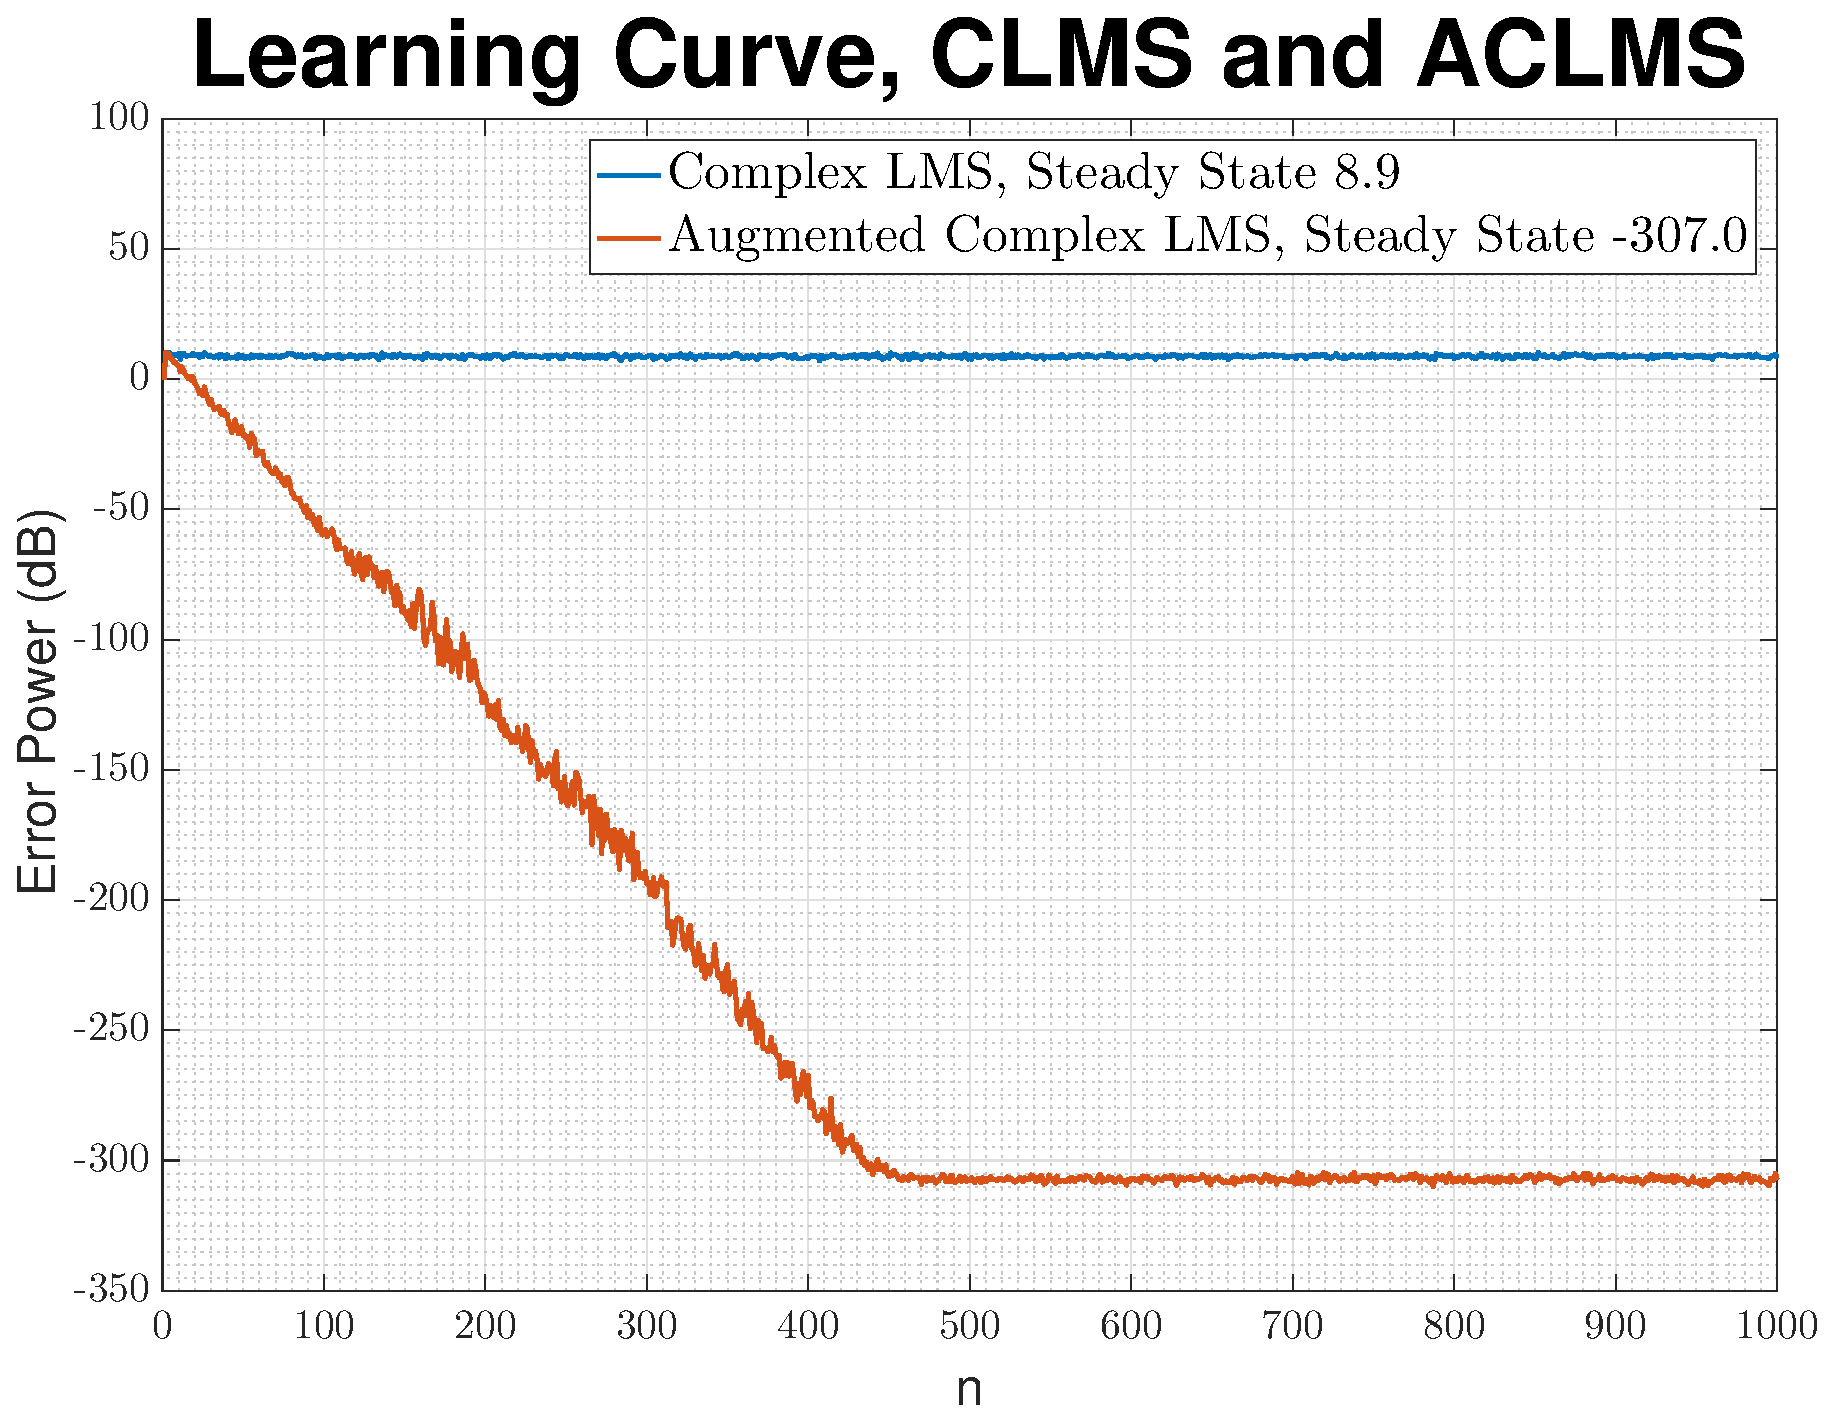
\includegraphics[width=0.32\textwidth]{part4/learning_curves_clms_aclms}
\caption{Comparison of Learning Curves using CLMS and ACLMS on Non-Circular WLMA(1) Process}
\end{figure}

\noindent{}b. Figure \ref{fig:wind_circularity} shows the scatter plots for the three wind regimes. A complex-valued random variable is said to be circular if its probability distribution is not dependent on the angle, that is, the distribution is rotation invariant. In other words the variable's probability distribution function should only depend on the Euclidean distance from the origin in the complex domain. The figure below also shows the circularity coefficient of each regime.\textbf{ It is of great importance to note that the higher the value of the circularity quotient, the less circular the data is.}

\begin{figure}[H]
\centering{}
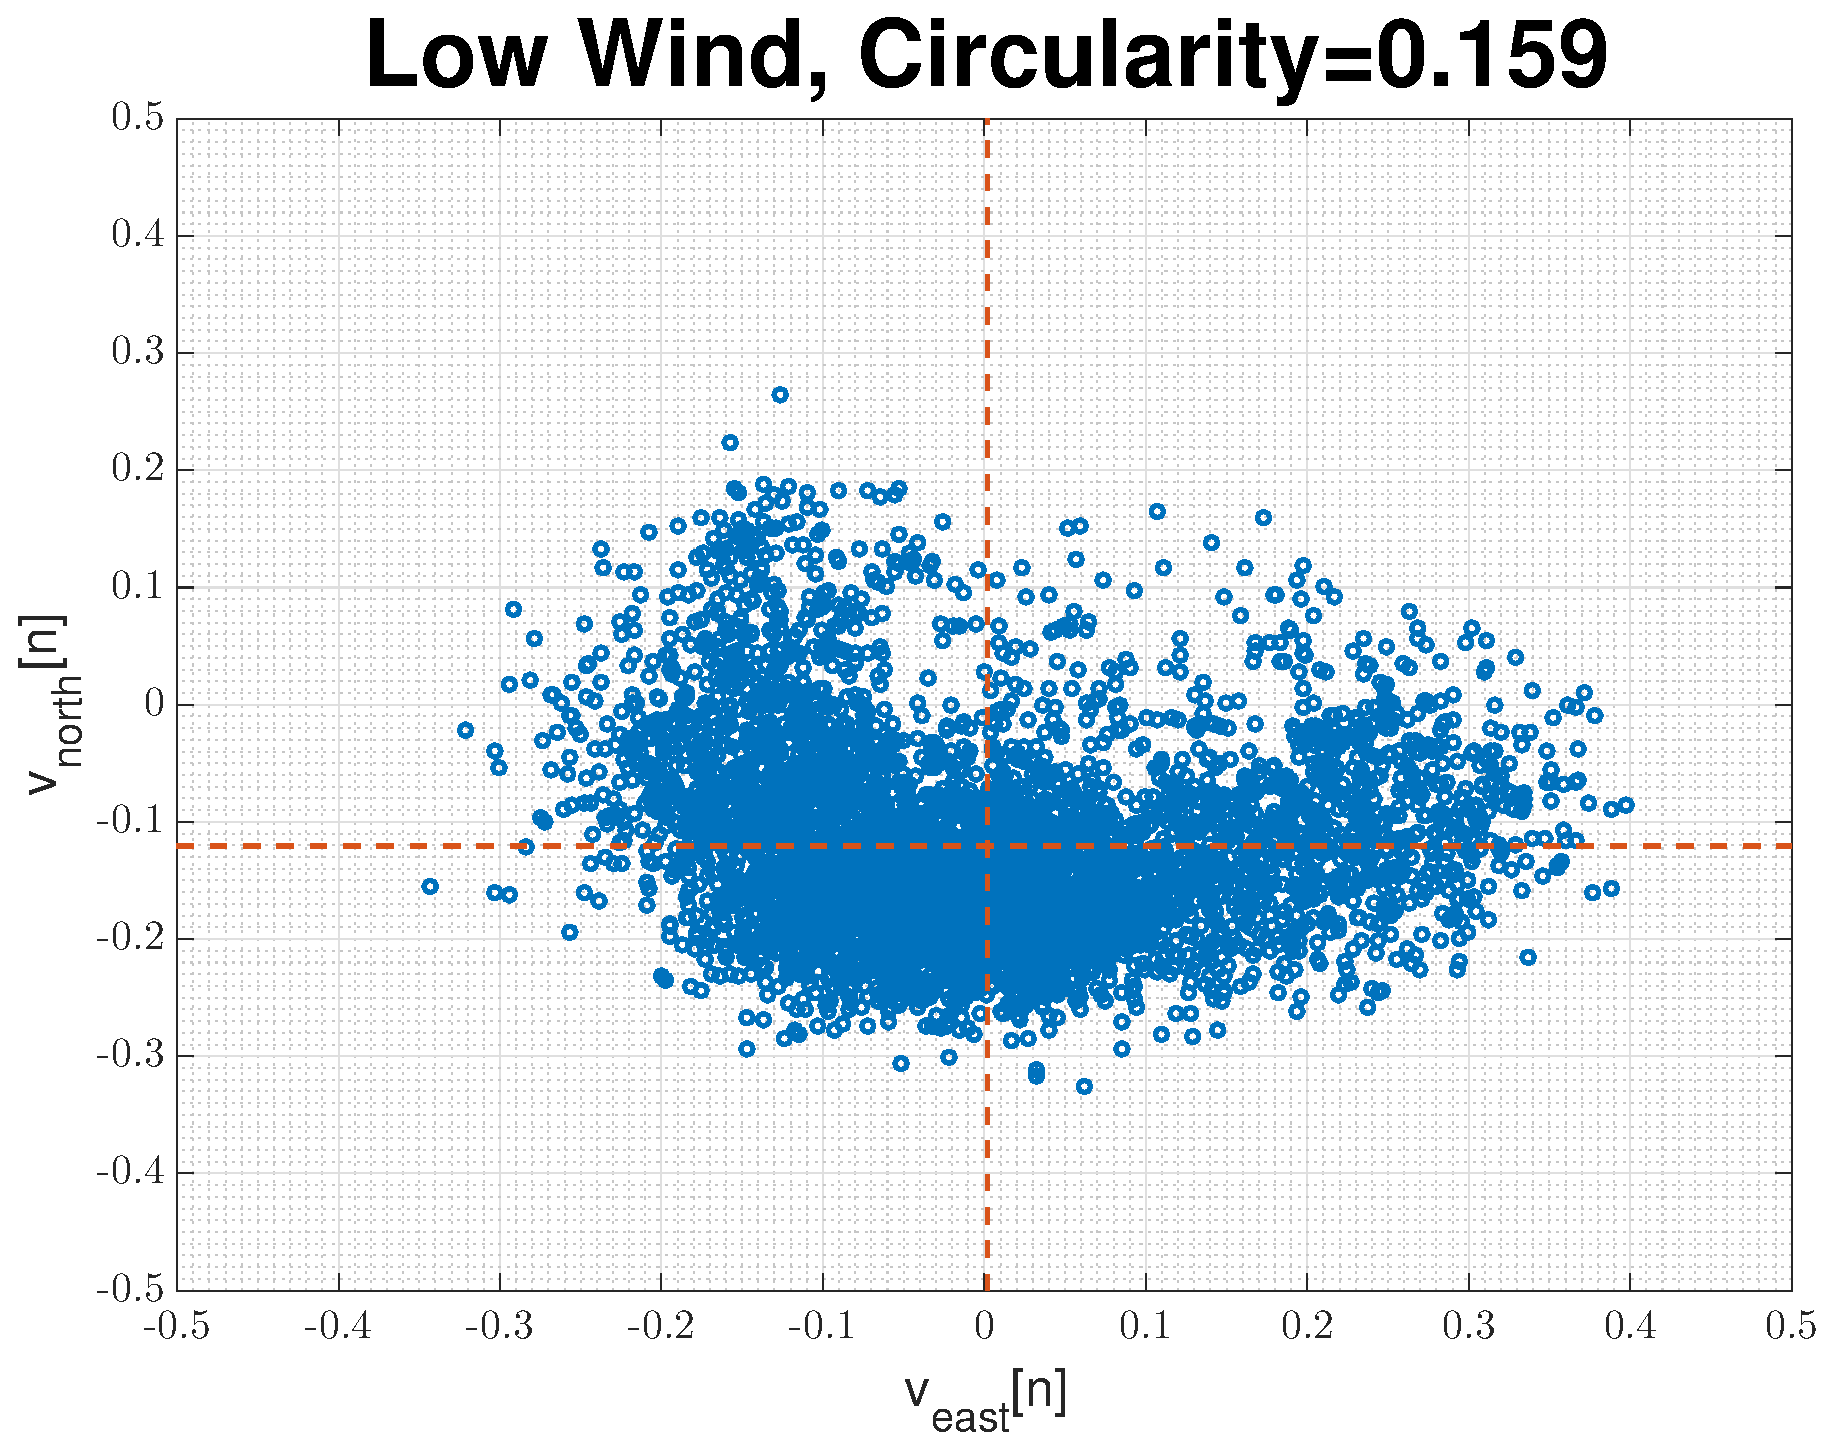
\includegraphics[width=0.32\textwidth]{part4/circularity_low_wind}
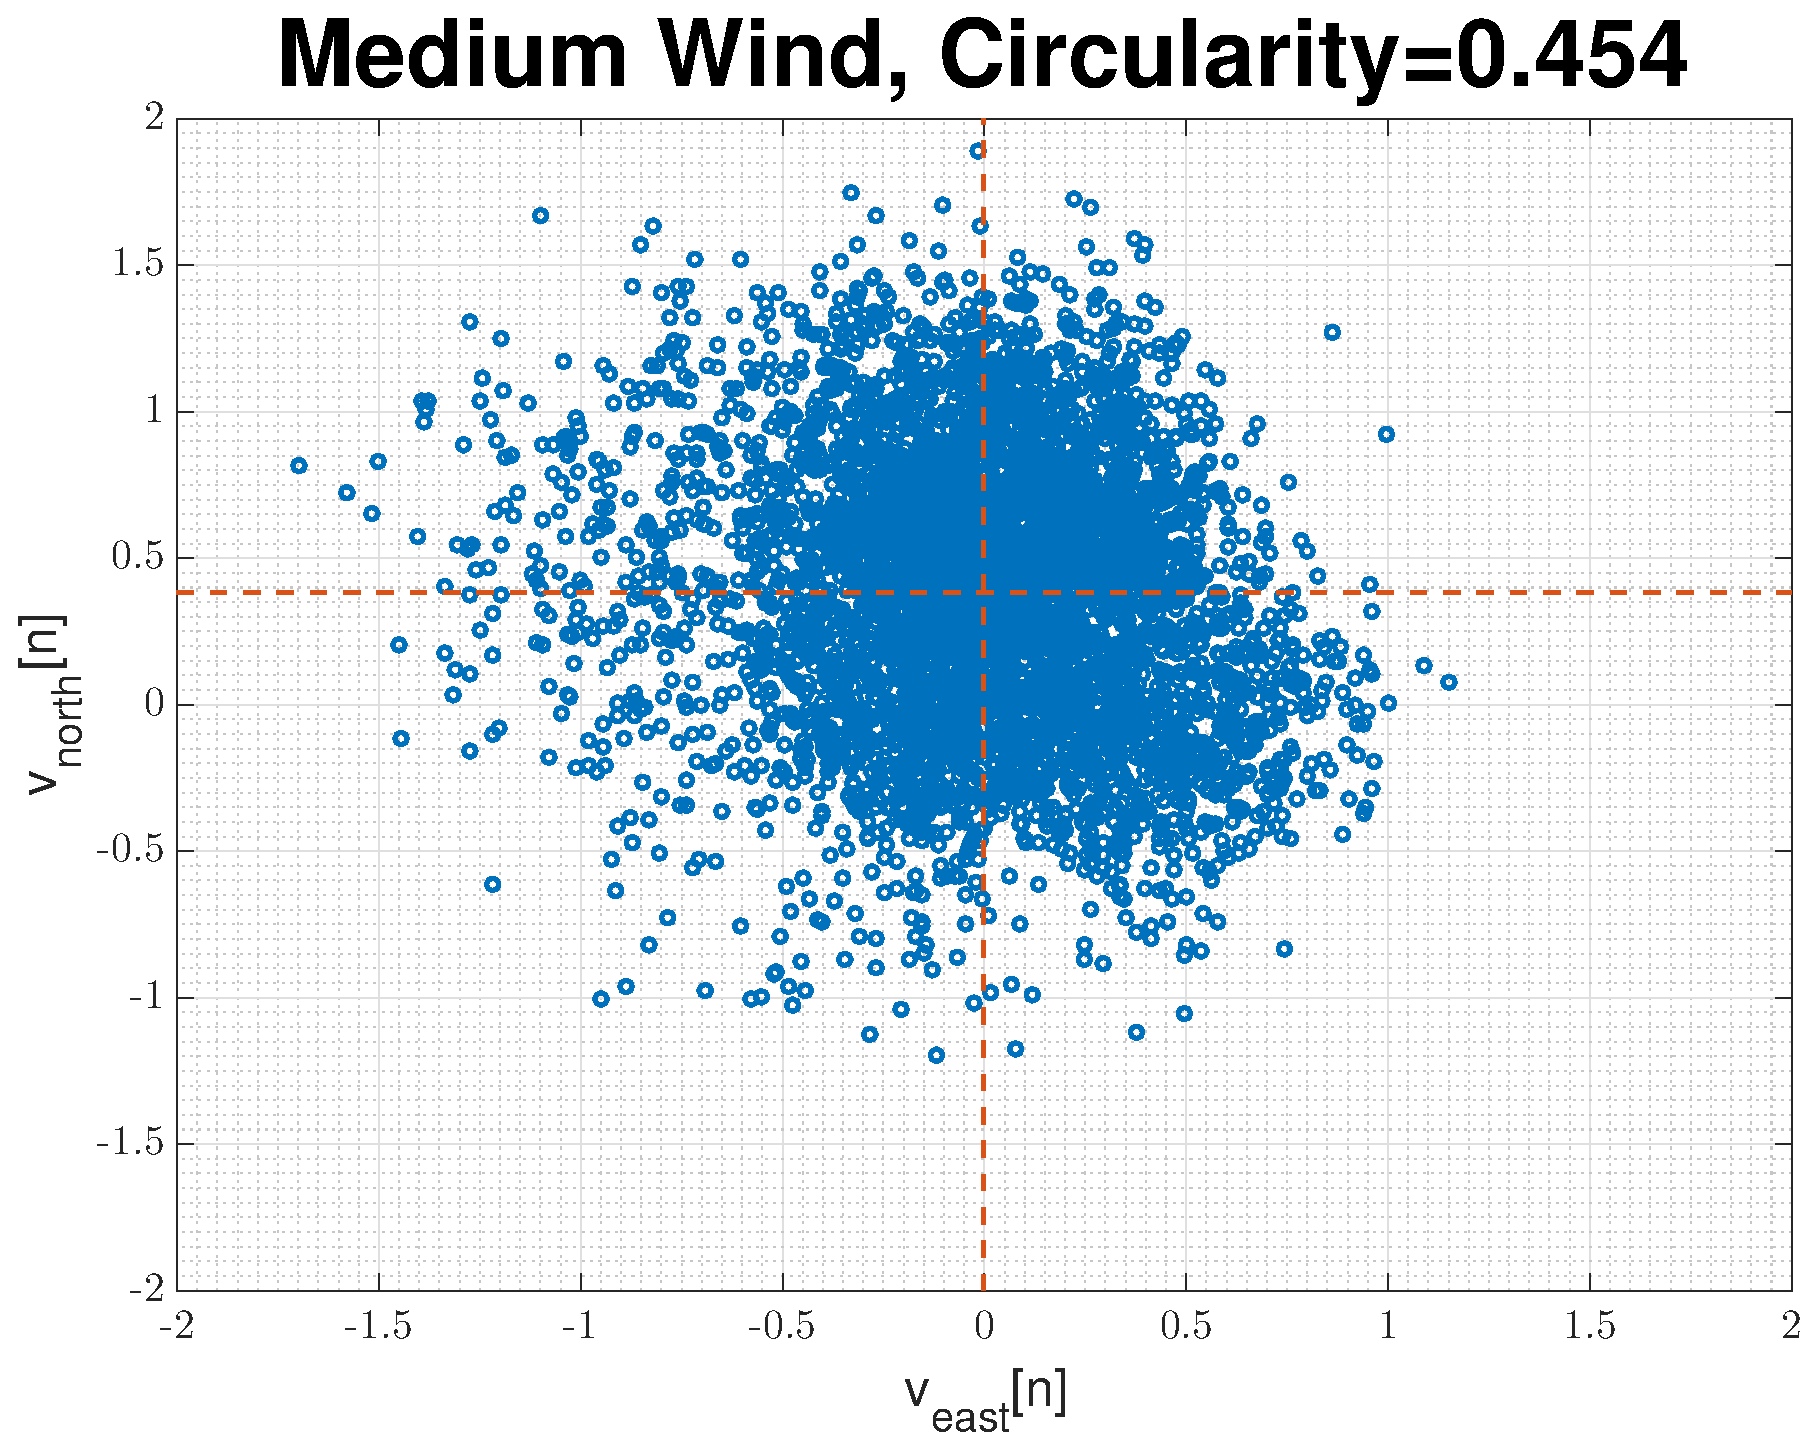
\includegraphics[width=0.32\textwidth]{part4/circularity_medium_wind}
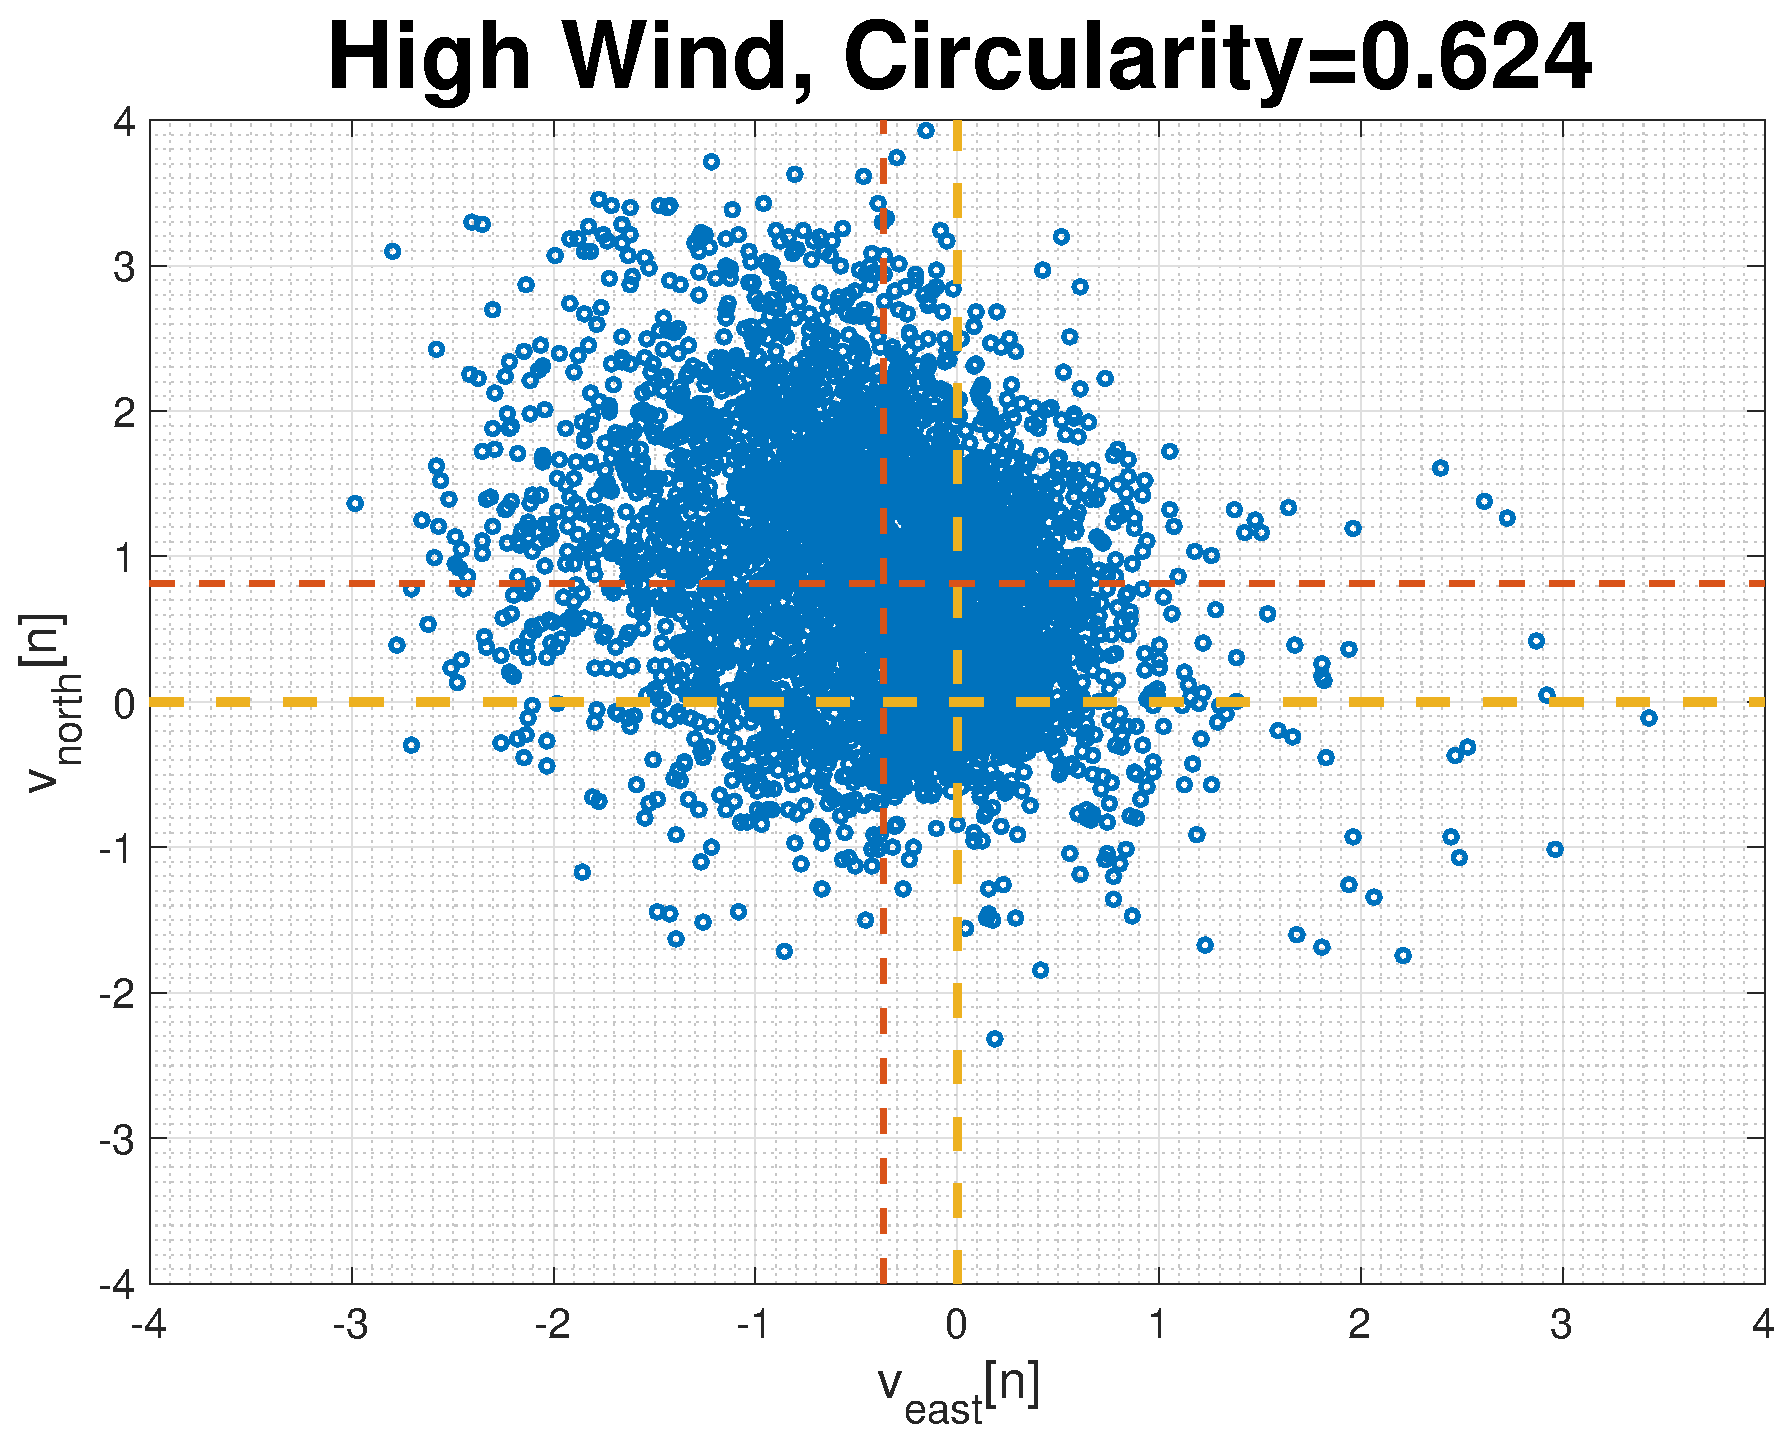
\includegraphics[width=0.32\textwidth]{part4/circularity_high_wind}
\caption{Circularity Plots for Different Wind Speeds}
\label{fig:wind_circularity}
\end{figure}

\noindent{}Now, looking at the graphs above without fully understanding the definition of circularity can lead to interpreting low-wind as being the least circular. It may seem that the low-wind regime is the least circular however upon closer inspection of the axis labels, it is clear that the high-wind regime has a big offset in its mean. The red dotted lines show the average values along each axis while the yellow dotted lines show the reference to the origin. The scatter plot for the high-wind regime is not centered around the origin and thus it is not rotation invariant. In contrast, although the low-wind regime does not appear circular, and looks slightly elliptical, the fact that its centered close to the origin means that it can be closely approximated to be circular. Each of the wind regimes was tested with the CLMS and the ACLMS algorithms and the results obtained are graphed in Figure \ref{fig:wind_order}.

\begin{figure}[H]
\centering{}
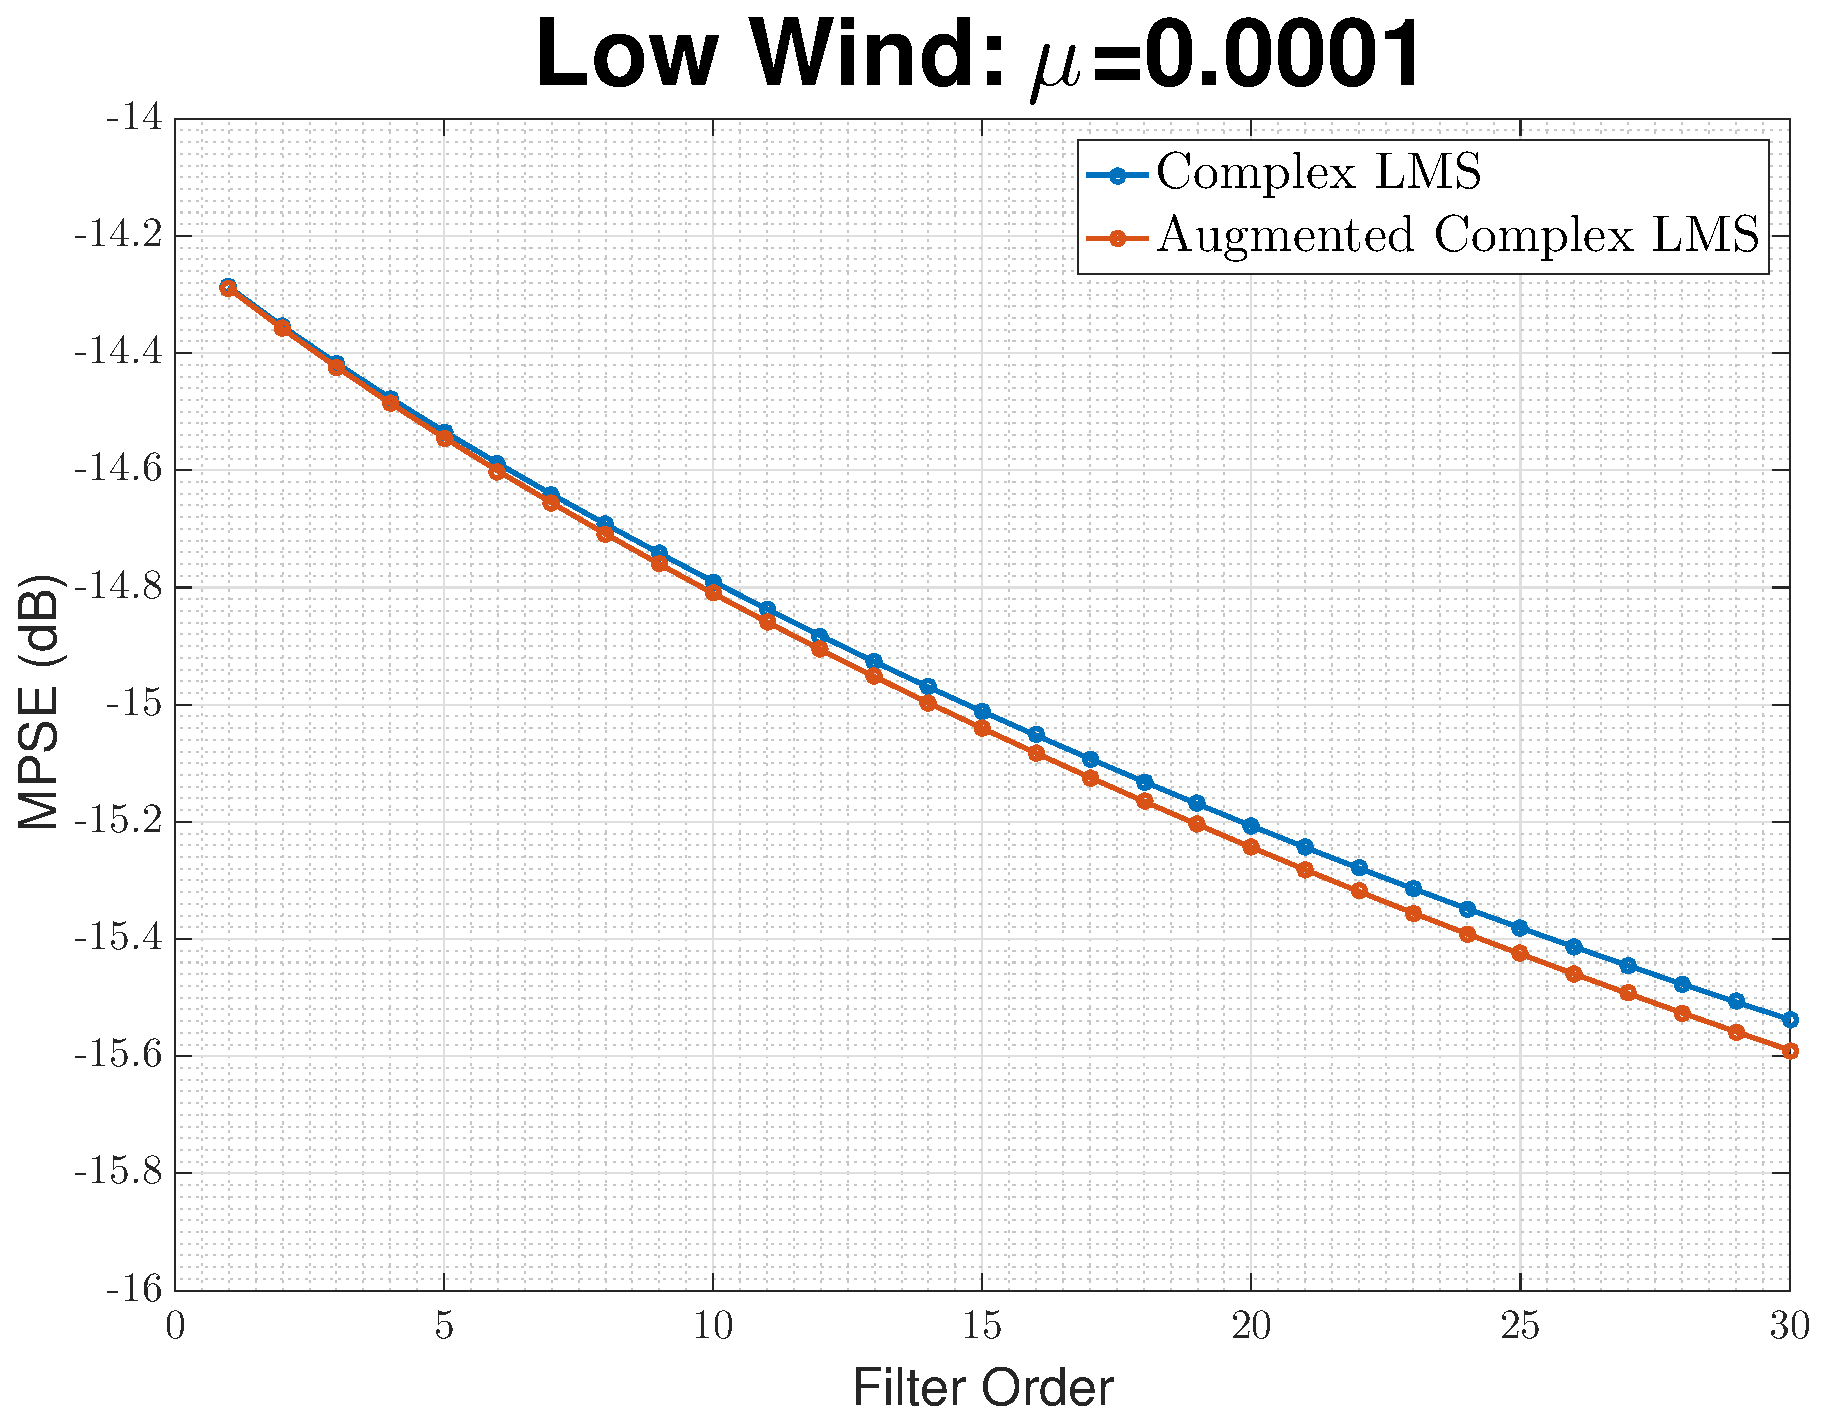
\includegraphics[width=0.32\textwidth]{part4/filt_order_low_wind}
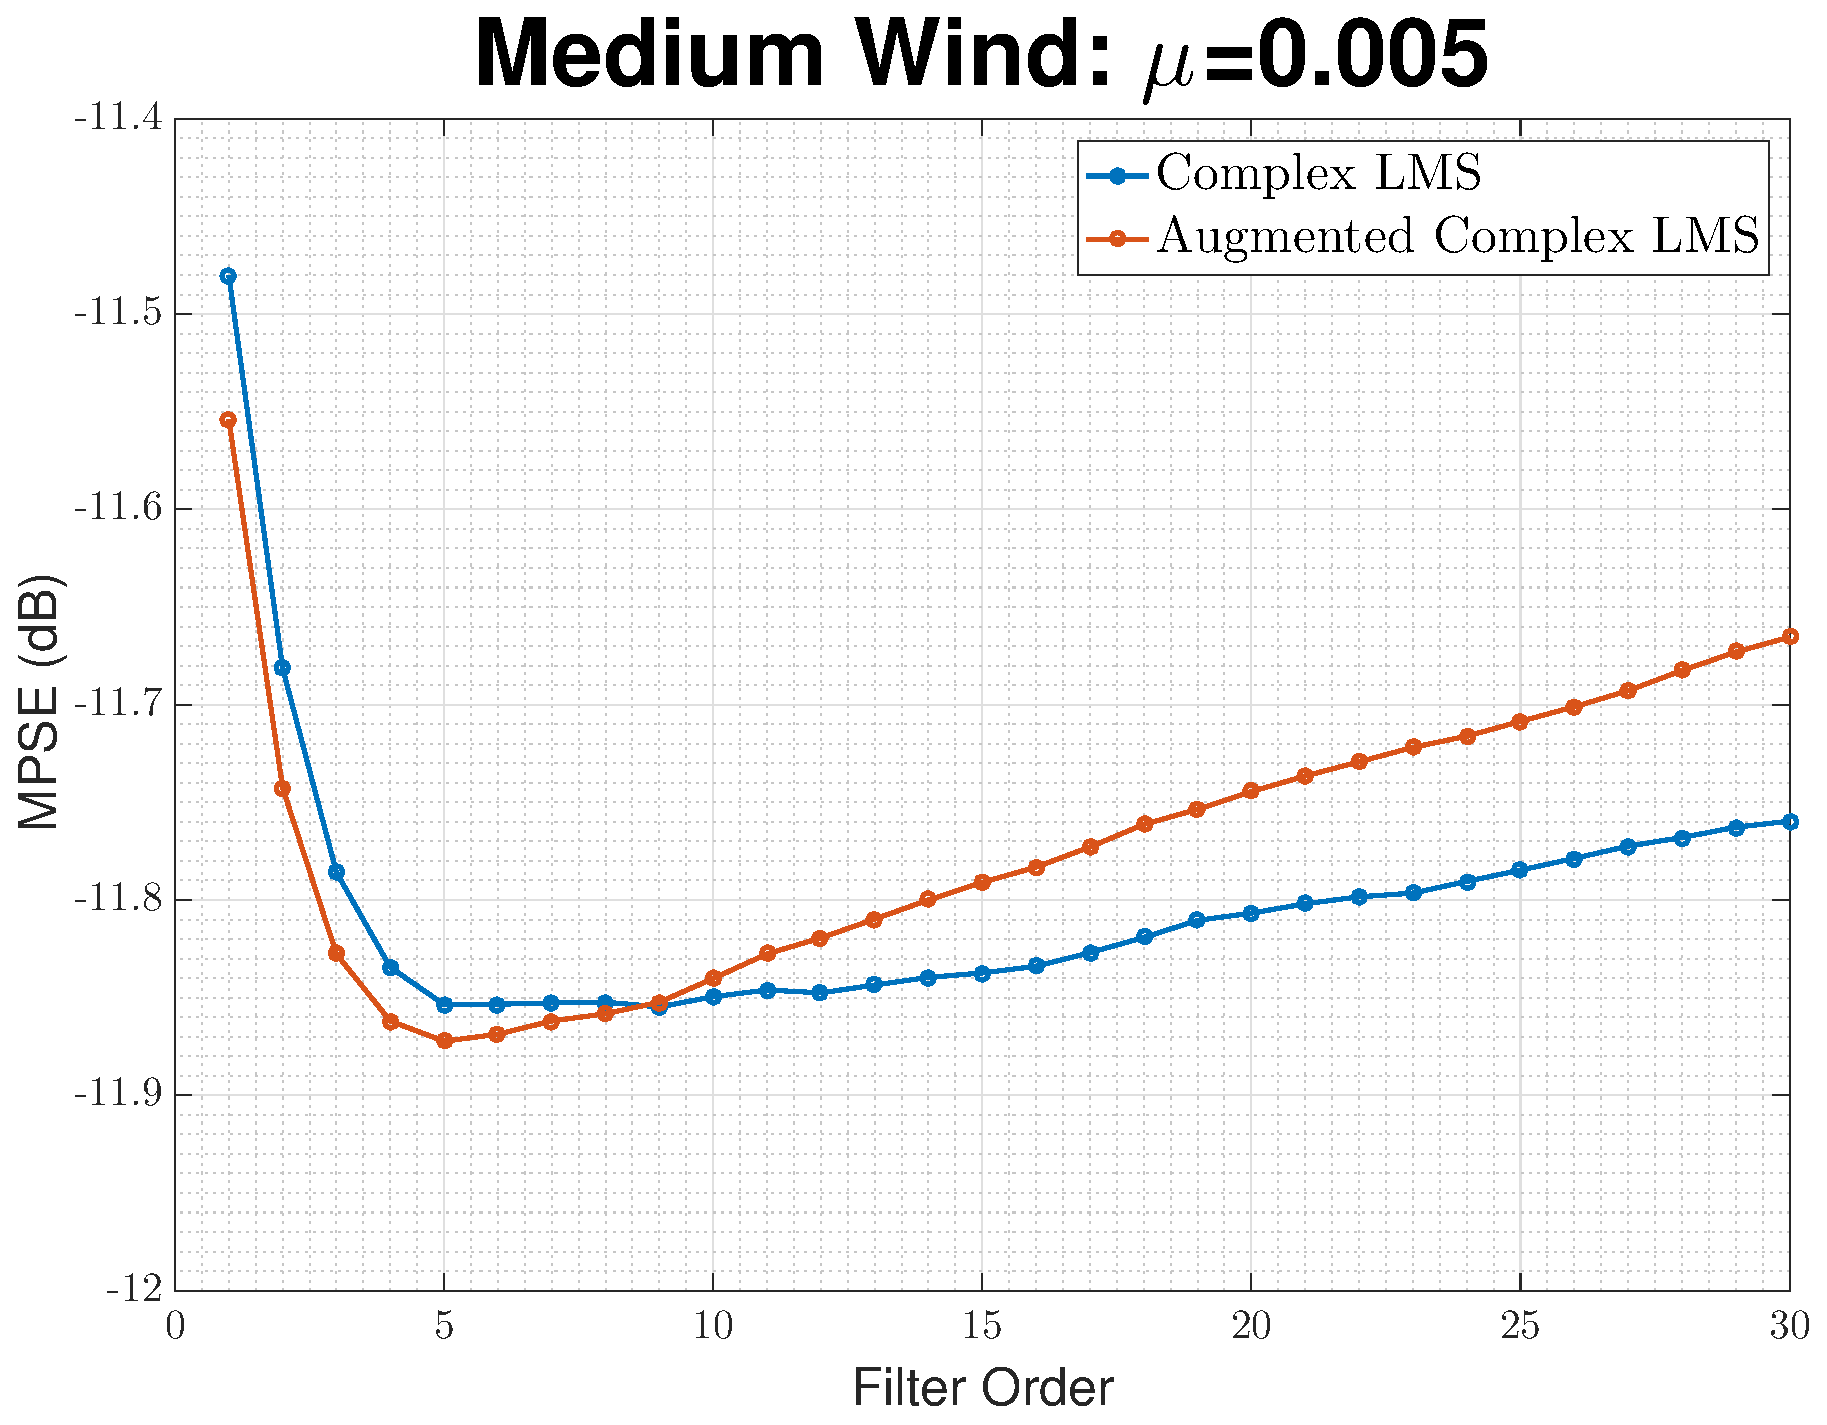
\includegraphics[width=0.32\textwidth]{part4/filt_order_medium_wind}
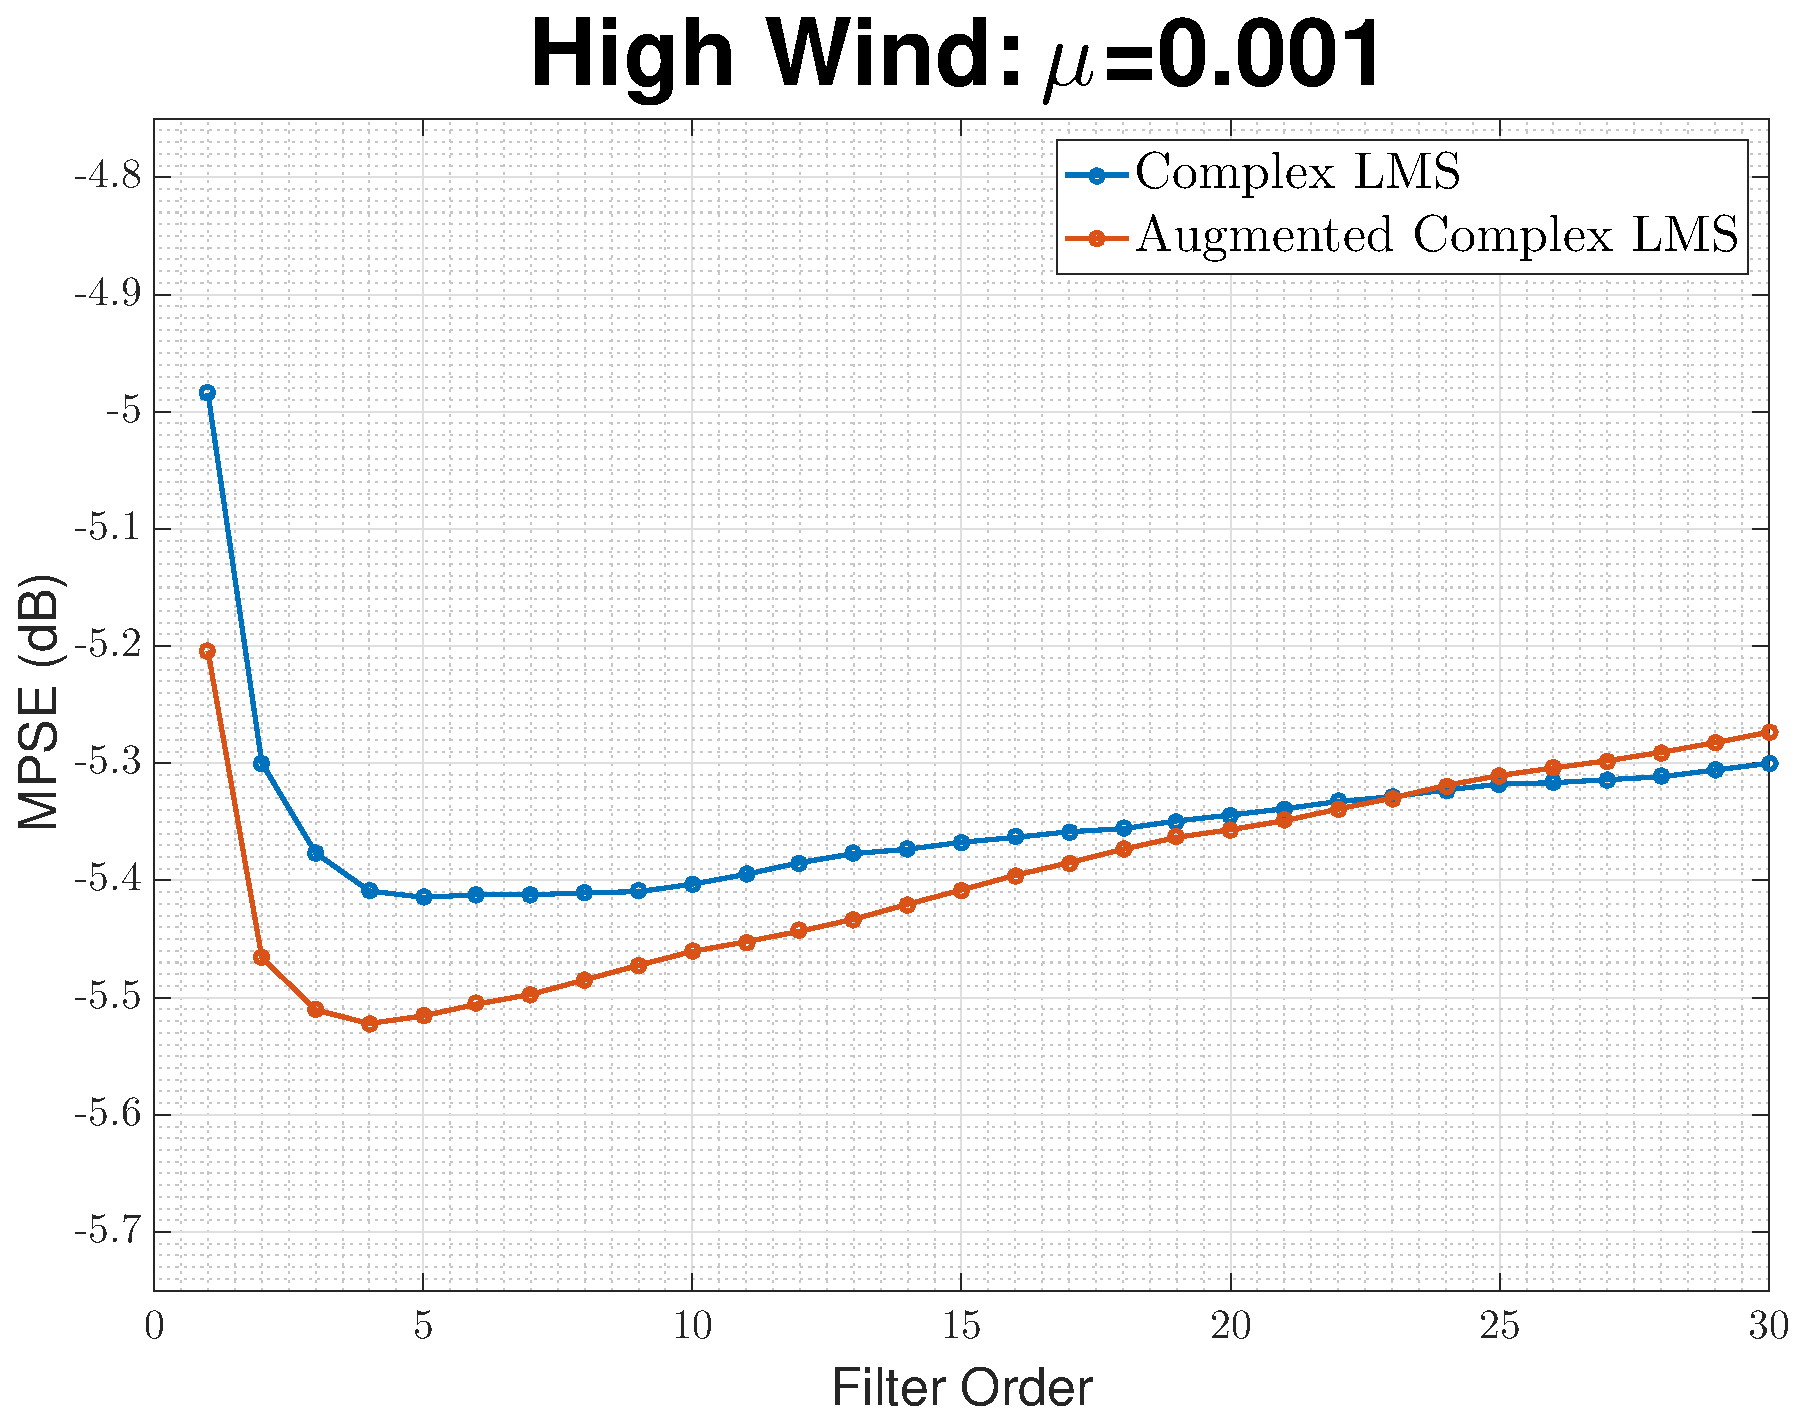
\includegraphics[width=0.32\textwidth]{part4/filt_order_high_wind}
\caption{Scaling of MPSE with Increase in Filter Order}
\label{fig:wind_order}
\end{figure}

\noindent{}The results are in accordance with the circularity coefficients of each regime for small model orders. The high and medium wind regimes do not perform well when one-step prediction is done using CLMS. The algorithm is not able to capture the non-circularity in the data. The low wind regime performs equally well using both the CLMS and ACLMS algorithms.\\

\noindent{}For higher model orders, the ACLMS algorithm's performance starts to degrade. This is due to the fact that overfitting starts to take place. The ACLMS algorithm has a greater number of parameters to tune as compared to the CLMS algorithm. The greater number of parameters affords the algorithm the ability to fit the training data extremely well. However, overfitting the data has the disadvantage that the filter will no longer generalize well, or in this case, predict future values well. The CLMS algorithm also clearly overfits the data since the prediction error starts to rise as the model order increases but the rate of overfitting is slower; this is again due to the fact that the CLMS algorithm has fewer parameters to tune. \\

\noindent{}c. The complex voltages in  the three-phase power system can be expressed compactly using the Clarke Transform reproduced in (\ref{eq:clarke_transform}).

\begin{align}
v(n) = A(n)e^{j\big(2\pi\frac{f_0}{f_s}n+\phi\big)} + B(n)e^{-j\big(2\pi\frac{f_0}{f_s}n+\phi\big)} \label{eq:clarke_transform}
\end{align}

\noindent{}where, $A(n)$ and $B(n)$ are as follows:

\begin{align*}
A(n) &= \frac{\sqrt{6}}{6}\bigg(V_a(n)+V_b(n)e^{j\Delta_b}+V_c(n)e^{j\Delta_c}\bigg) \\
B(n) &= \frac{\sqrt{6}}{6}\bigg(V_a(n)+V_b(n)e^{-j(\Delta_b + \frac{2\pi}{3})}+V_c(n)e^{-j(\Delta_c-\frac{2\pi}{3})}\bigg)
\end{align*}

\noindent{}For the system to be balanced, $B(n)$ must be equal to 0. This is only possible if two conditions are met. Firstly, all the voltages must have the same magnitudes, such that $V_a(n)=V_b(n)=V_c(n)$. Secondly, the phase difference between each of the three signals must be fixed. This is achieved when $\Delta_b=\Delta_c=0$. These two conditions thus give us 2 ways to unbalance the system. The figure below shows a balanced signal, variations of signals that have been unbalanced by changing the relative magnitudes of each component and also variations of signals that have been unbalanced by changing the phase difference between each component.  
\begin{figure}[H]
\centering{}
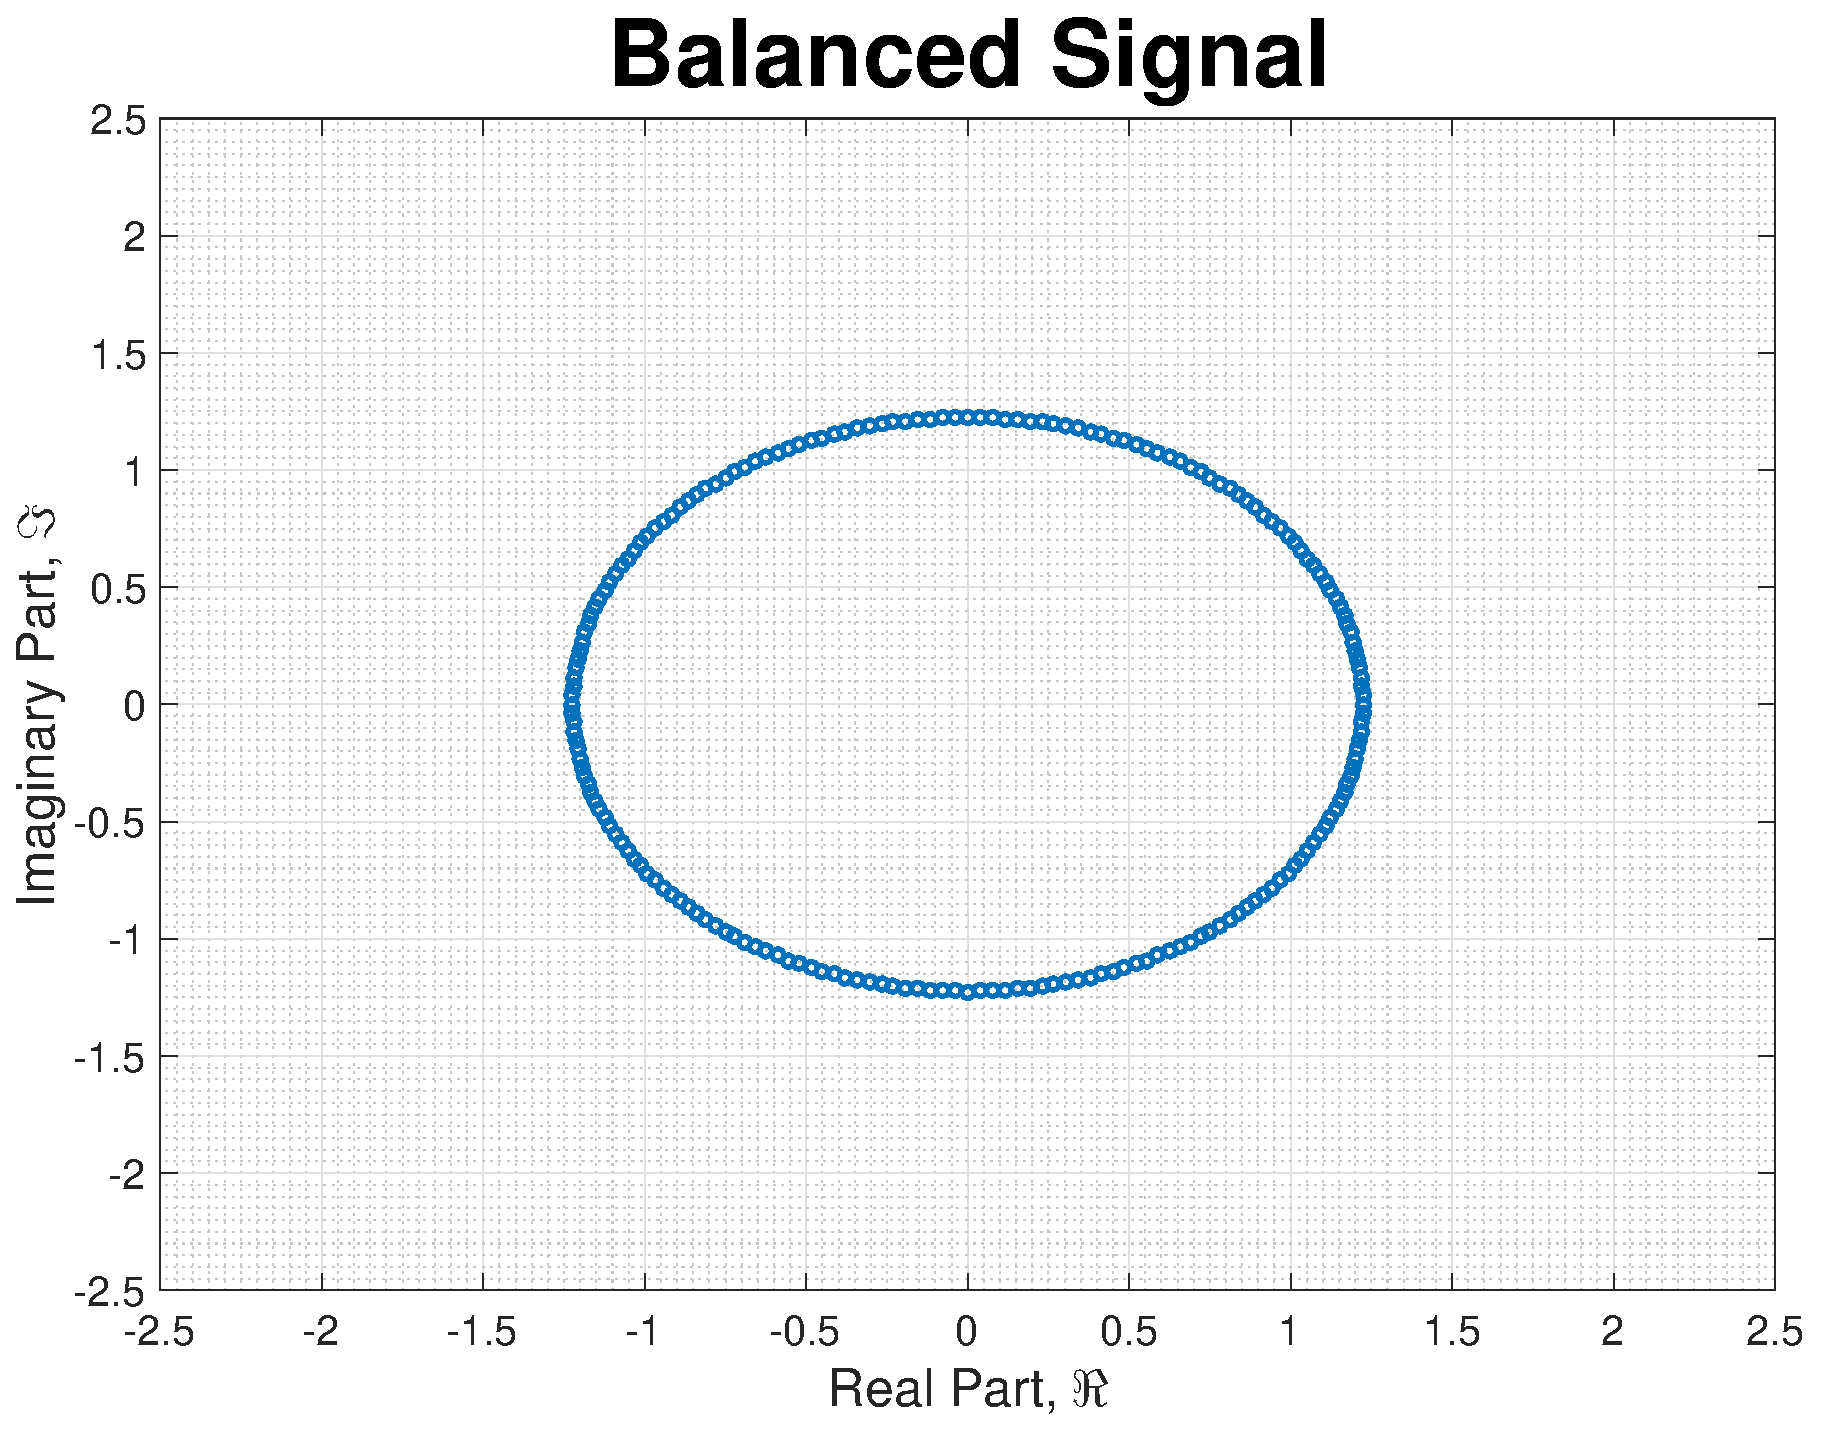
\includegraphics[width=0.32\textwidth]{part4/balanced_signal}
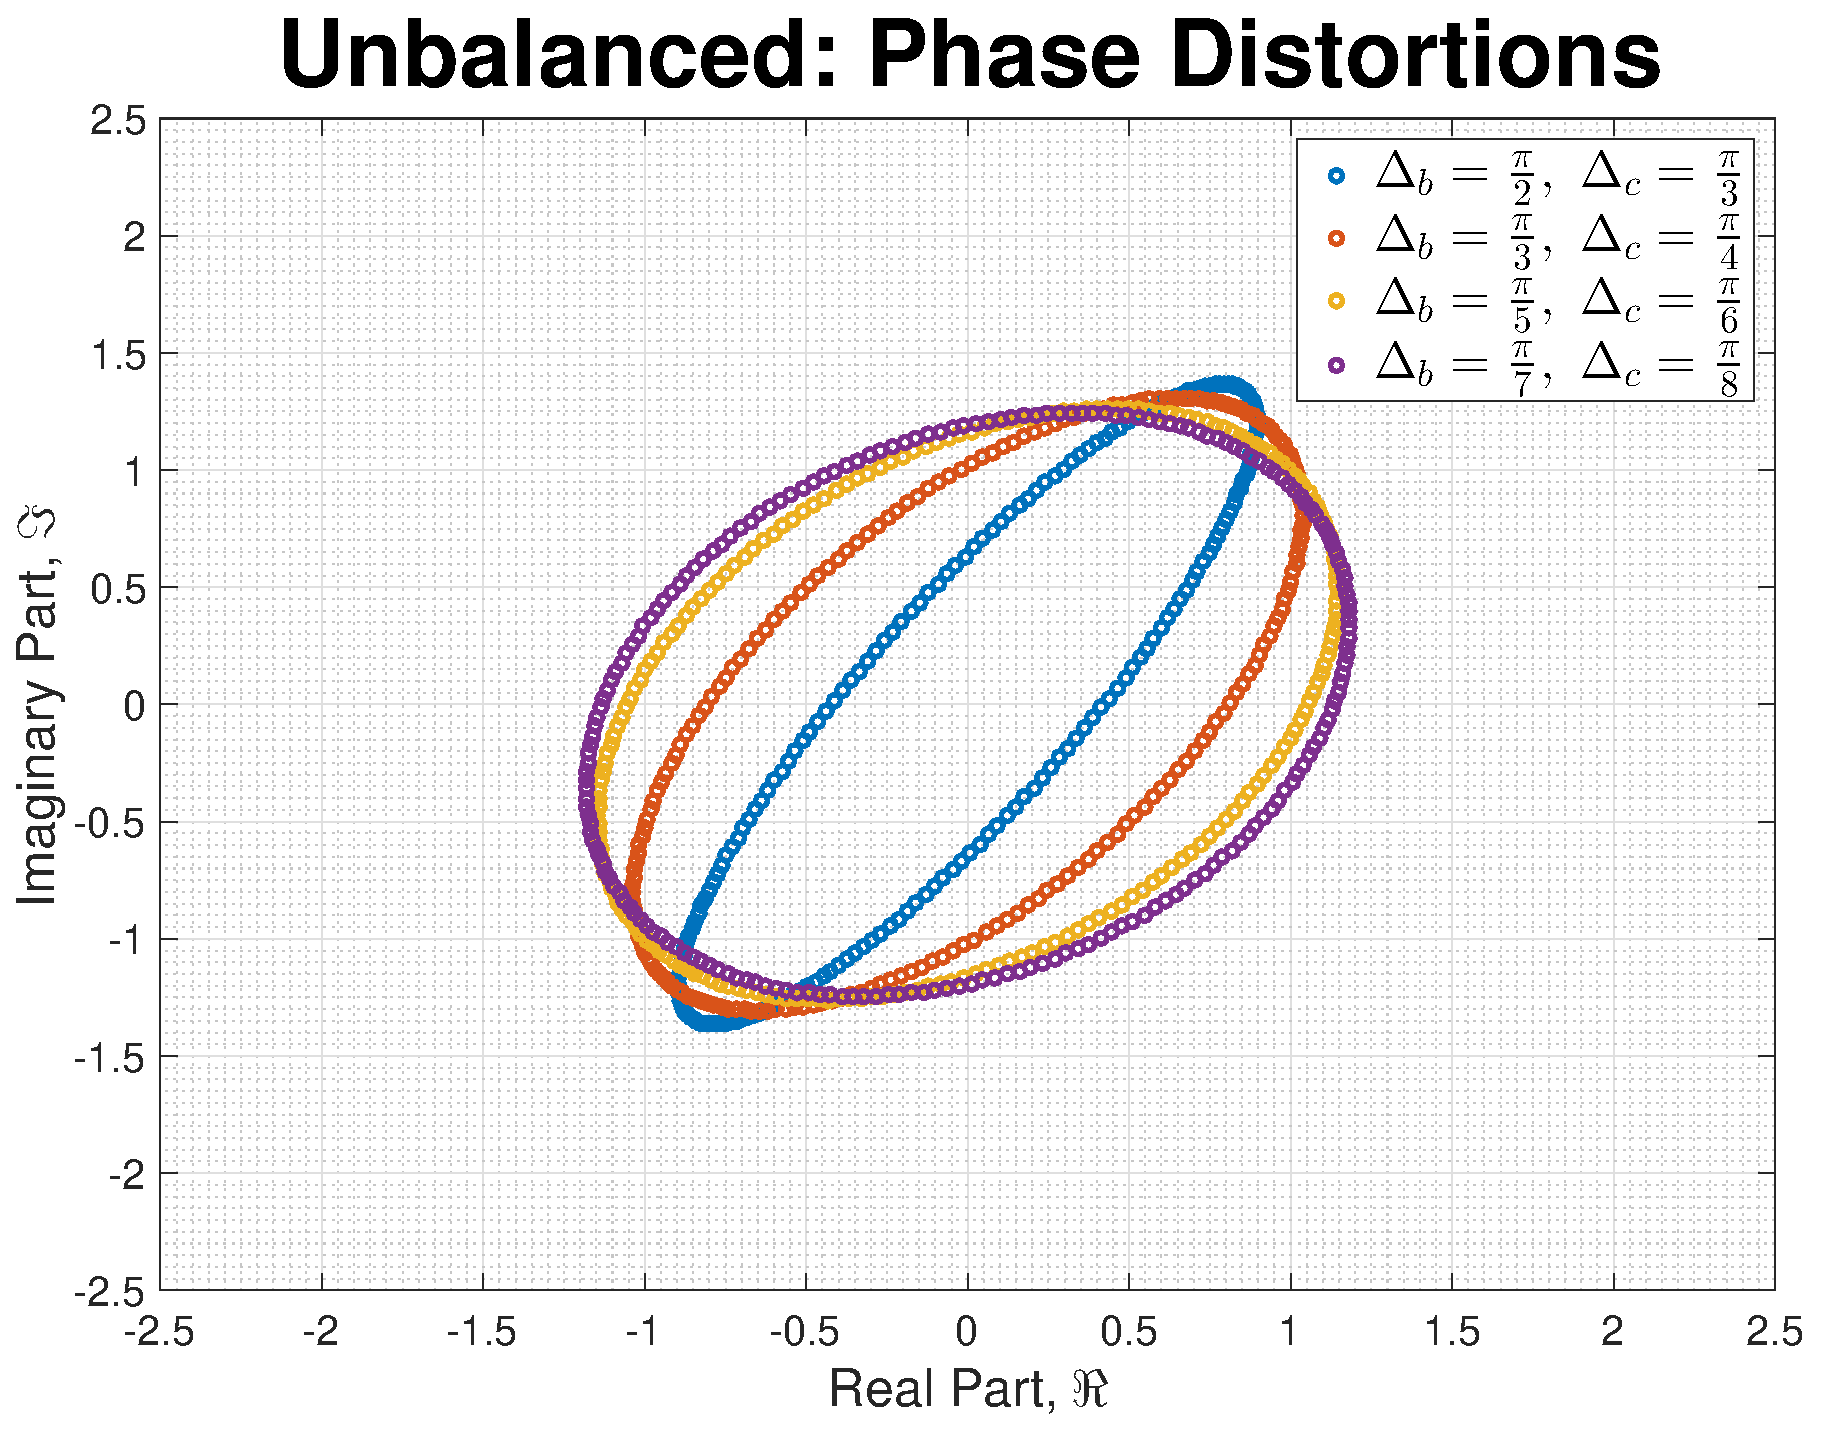
\includegraphics[width=0.32\textwidth]{part4/unbalanced_phase_distortion}
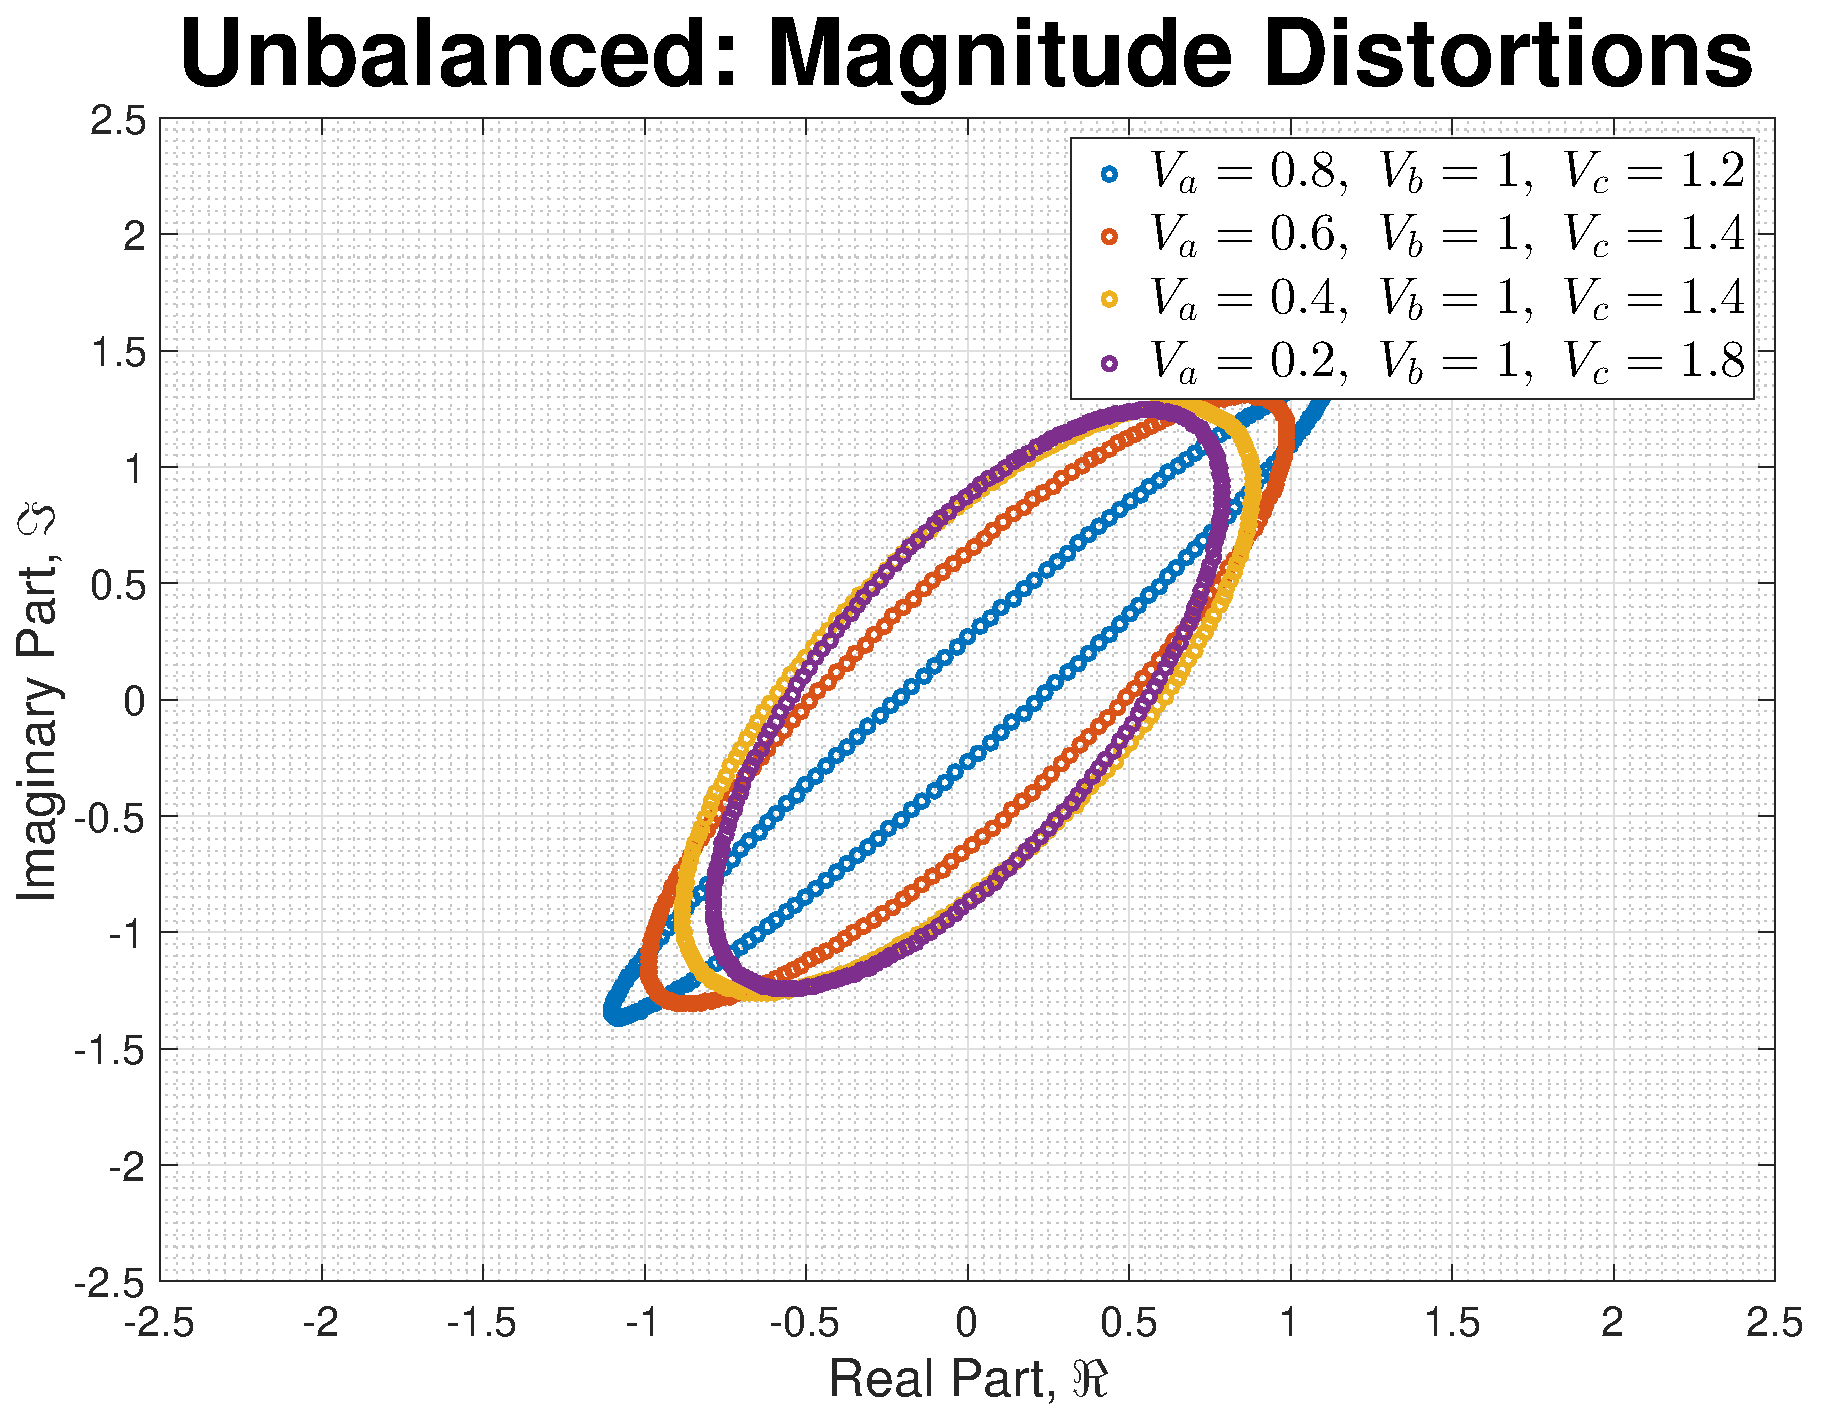
\includegraphics[width=0.32\textwidth]{part4/unbalanced_magnitude_distortion}
\caption{Balanced and Unbalanced Complex Voltages}
\end{figure}

\noindent{}It is clear that we can visually when a system is balanced as compared to when it is unbalanced. A balanced system results in a circular plot, whereas an unbalanced system does not. In fact, patterns can also be drawn about the effects of changing the relative magnitudes or phase differences.\\

\noindent{}c. A strictly linear first order autoregressive model has the form given in (\ref{eq:ar_strict_linear}). 

\begin{align}
v(n+1)=h*(n)v(n) \label{eq:ar_strict_linear}
\end{align}

\noindent{}Next, given that:

\begin{align*}
v(n) = \sqrt{\frac{3}{2}}Ve^{j\big(2\pi\frac{f_0}{f_s}n+\phi\big)}
\end{align*}

\noindent{}We can rearrange (\ref{eq:ar_strict_linear}) to give:

\begin{align*}
\frac{\sqrt{\frac{3}{2}}Ve^{j\big(2\pi\frac{f_0}{f_s}(n+1)+\phi\big)}}{\sqrt{\frac{3}{2}}Ve^{j\big(2\pi\frac{f_0}{f_s}n+\phi\big)}} = h^*(n)
\end{align*}

\noindent{}Simplifying the left-hand side followed by replacing $h^*(n)$ with $h(n)$:

\begin{align*}
e^{j2\pi\frac{f_0}{f_s}} &= h^*(n)\\
&=\Re\{h(n)\} - \Im\{h(n)\} \\
&=|h(n)|e^{-j\big(\text{arctan}\big(\frac{\Re\{h(n)\}}{\Im\{h(n)\}}\big)\big)}
\end{align*}

\noindent{}Next, equating only the phase of the left and right hand sides:

\begin{align*}
2\pi\frac{f_0}{f_s} = -\text{arctan}\bigg(\frac{\Re\{h(n)\}}{\Im\{h(n)\}}\bigg)
\end{align*}

\noindent{}Bringing the minus sign into the arctan by taking the reciprocal of the fraction, then rearranging, we get (\ref{eq:ar_strict_linear_final}) which completes the proof.

\begin{align}
f_0 = \frac{f_s}{2\pi}\text{arctan}\bigg(\frac{\Im\{h(n)\}}{\Re\{h(n)\}}\bigg) \label{eq:ar_strict_linear_final}
\end{align}

\noindent{}For the unbalanced system, we start with the widely linear first order autoregressive model which has the form given in (\ref{eq:widely_lin_ar}).

\begin{align}
v(n+1) = h^*(n)v(n) + g^*(n) v^*(n) \label{eq:widely_lin_ar}
\end{align}

\noindent{}Next, given that:

\begin{align*}
v(n) = A(n)e^{j\big(2\pi\frac{f_0}{f_s}n+\phi\big)} + B(n)e^{-j\big(2\pi\frac{f_0}{f_s}n+\phi\big)}
\end{align*}

\noindent{}We substitute $v(n)$ and $v^*(n)$ in (\ref{eq:widely_lin_ar}):

\begin{align*}
v(n+1) = h^*(n)A(n)e^{j\big(2\pi\frac{f_0}{f_s}n+\phi\big)} + h^*(n)B(n)e^{-j\big(2\pi\frac{f_0}{f_s}n+\phi\big)} + g^*(n)A^*(n)e^{-j\big(2\pi\frac{f_0}{f_s}n+\phi\big)} + g^*(n)B^*(n)e^{j\big(2\pi\frac{f_0}{f_s}n+\phi\big)}
\end{align*}

\noindent{}Next, we know that:

\begin{align*}
v(n+1) = A(n+1)e^{j\big(2\pi\frac{f_0}{f_s}(n+1)+\phi\big)} + B(n+1)e^{-j\big(2\pi\frac{f_0}{f_s}(n+1)+\phi\big)}
\end{align*}

\noindent{}We can now substitute $v(n+1)$ in (\ref{eq:widely_lin_ar}). We then simplify and group exponential terms together and get the following equations:

\begin{align*}
A(n+1)e^{j\big(2\pi\frac{f_0}{f_s}(n+1)+\phi\big)} &= \big(h^*(n)A(n)+g^*(n)B^*(n)\big)e^{j\big(2\pi\frac{f_0}{f_s}n+\phi\big)} \\
B(n+1)e^{-j\big(2\pi\frac{f_0}{f_s}(n+1)+\phi\big)} &= \big(h^*(n)B(n)+g^*(n)A^*(n)\big)e^{-j\big(2\pi\frac{f_0}{f_s}n+\phi\big)}
\end{align*}

\noindent{}Next, making the assumption that $A(n+1)\approx A(n)$ and $B(n+1)\approx B(n)$, we can simplify the above equations to:

\begin{align}
e^{j2\pi\frac{f_0}{f_s}} &= \frac{h^*(n)A(n)+g^*(n)B^*(n)}{A(n+1)} \approx h^*(n) + g^*(n)\frac{B^*(n)}{A(n)} \label{eq:widely_mid_1}\\
e^{-j2\pi\frac{f_0}{f_s}} &= \frac{h^*(n)B(n)+g^*(n)A^*(n)}{B(n+1)} \approx h^*(n) + g^*(n)\frac{A^*(n)}{B(n)} \nonumber
\end{align}

\noindent{}Taking conjugates and equating:

\begin{align*}
h^*(n) + g^*(n)\frac{B^*(n)}{A(n)} = h(n) + g(n)\frac{A(n)}{B^*(n)} 
\end{align*}

\noindent{}Next, setting $Y=\frac{A(n)}{B^*(n)}$, we get a quadratic equation in $Y$:

\begin{align*}
g^*(n)Y^2 + \big(h^*(n)-h(n)\big)Y + g(n) = 0
\end{align*}

\noindent{}Solving for $Y$, we get:

\begin{align*}
Y &= \frac{-\big(h^*(n)-h(n)\big) \pm \sqrt{\big(h^*(n)-h(n)\big)^2-4g^*(n)g(n)}}{2g^*(n)} \\
&= \frac{2\Im\{h(n)\}j \pm \sqrt{-4\Im^2\{h(n)\}+4|g(n)|^2}}{2g^*(n)} \\
&= \frac{2\Im\{h(n)\}j \pm j\sqrt{4\Im^2\{h(n)\}-4|g(n)|^2}}{2g^*(n)}
\end{align*}

\noindent{}Substituting $Y$ into (\ref{eq:widely_mid_1}), we obtain:

\begin{align*}
e^{j2\pi\frac{f_0}{f_s}} &= h^*(n) + 2\Im\{h(n)\}j \pm j\sqrt{4\Im^2\{h(n)\}-4|g(n)|^2} \\
&= \Re\{h(n)\} \pm j\sqrt{4\Im^2\{h(n)\}-4|g(n)|^2}
\end{align*}

\noindent{}Since $f_s > f_0 > 0$:

\begin{align*}
e^{j2\pi\frac{f_0}{f_s}}  &= \Re\{h(n)\} + j\sqrt{4\Im^2\{h(n)\}-4|g(n)|^2} \\
&= |M| e^{j\big(\text{arctan}\big(\frac{\sqrt{4\Im^2\{h(n)\}-4|g(n)|^2}}{\Re\{h(n)\}}\big)\big)}
\end{align*}

\noindent{}Next, equating only the phase of the left and right hand sides:

\begin{align*}
2\pi\frac{f_0}{f_s}  &= \text{arctan}\bigg(\frac{\sqrt{4\Im^2\{h(n)\}-4|g(n)|^2}}{\Re\{h(n)\}}\bigg)
\end{align*}

\noindent{}Rearranging, we get (\ref{eq:widely_lin_ar_final}) which completes the proof:

\begin{align}
f_0 = \frac{f_s}{2\pi} \text{arctan}\bigg(\frac{\sqrt{4\Im^2\{h(n)\}-4|g(n)|^2}}{\Re\{h(n)\}}\bigg) \label{eq:widely_lin_ar_final}
\end{align}

\noindent{}d. The value of $f_0$ was set at 50 Hz to match the operating frequency of power transmission in the UK. The figure below shows how the two algorithms perform when tested on a balanced system. The CLMS algorithm converges much faster than the ACLMS algorithm. The ACLMS also displays a big overshoot during the first two iterations, something that the CLMS algorithm does not do. Note that both algorithms converge to the nominal frequency of 50 Hz without any bias.

\begin{figure}[H]
\centering{}
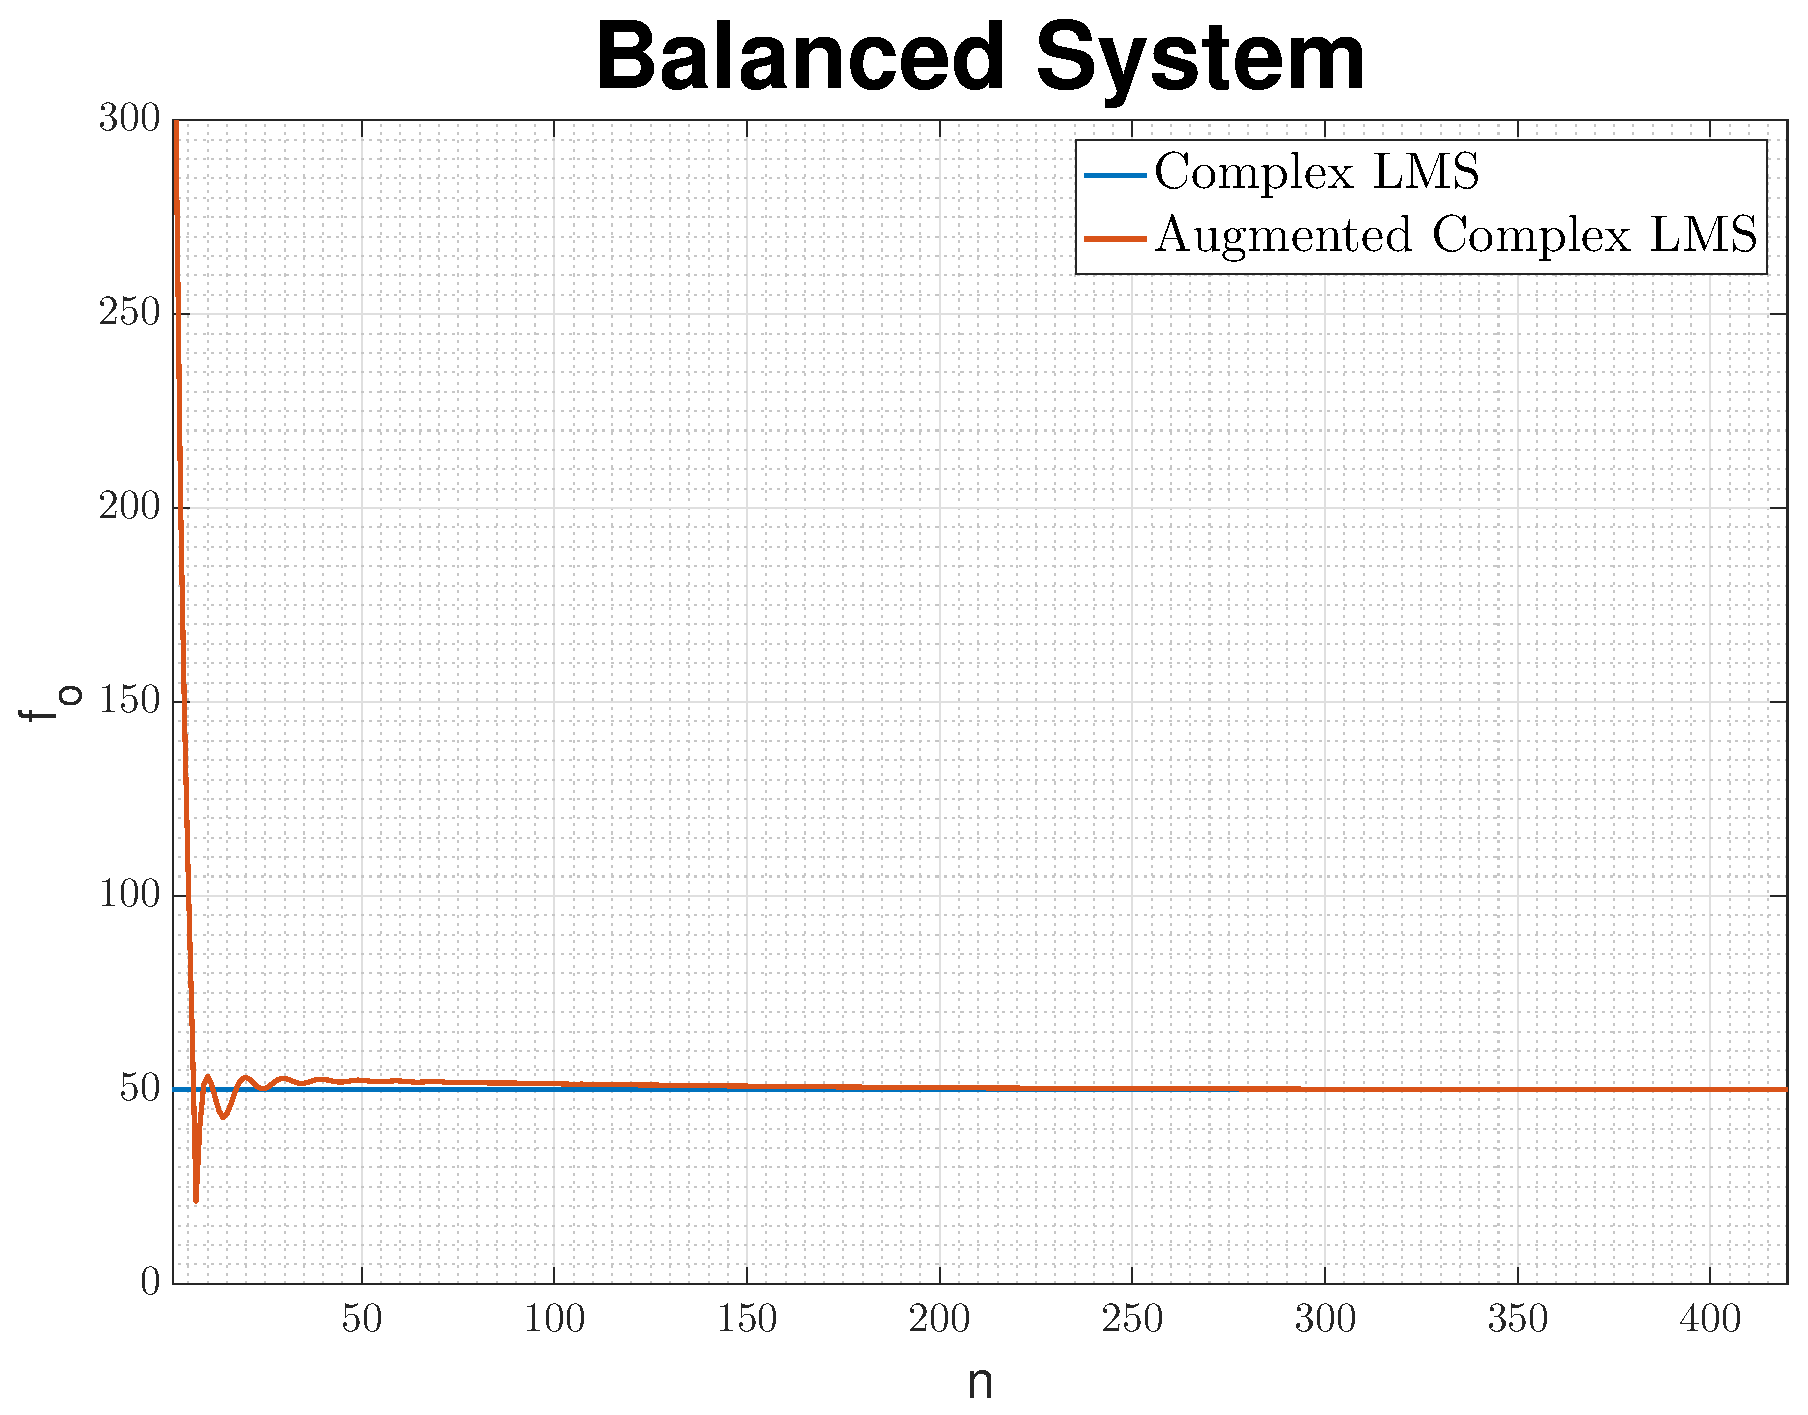
\includegraphics[width=0.32\textwidth]{part4/balanced_sys_clms_aclms}
\caption{Comparison of CLMS and ACLMS for Balanced Complex Voltages}
\end{figure}

\noindent{}

\begin{figure}[H]
\centering{}
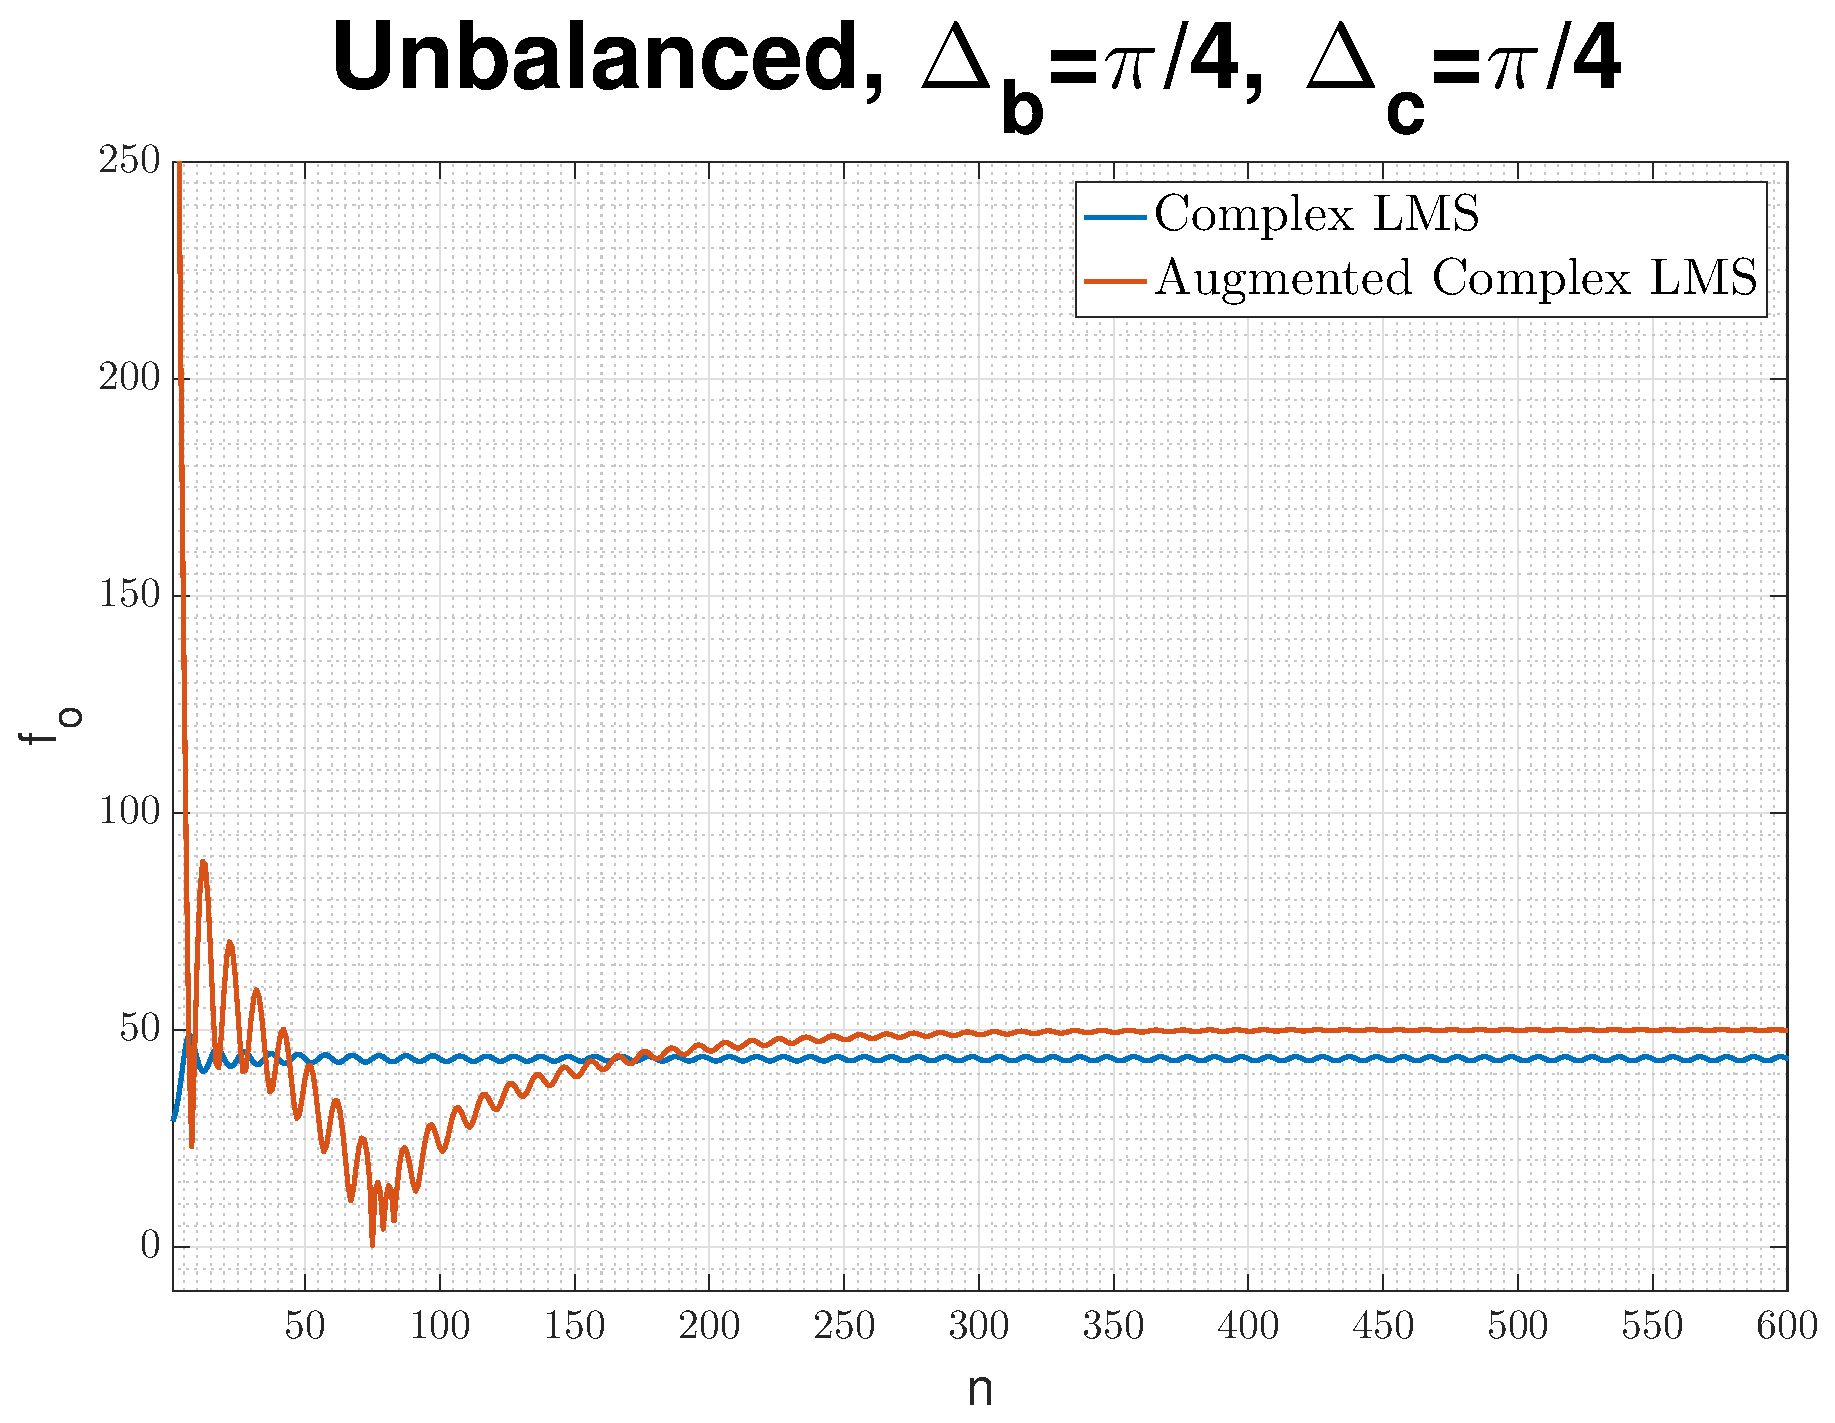
\includegraphics[width=0.32\textwidth]{part4/unbalanced_sys_clms_aclms_phase}
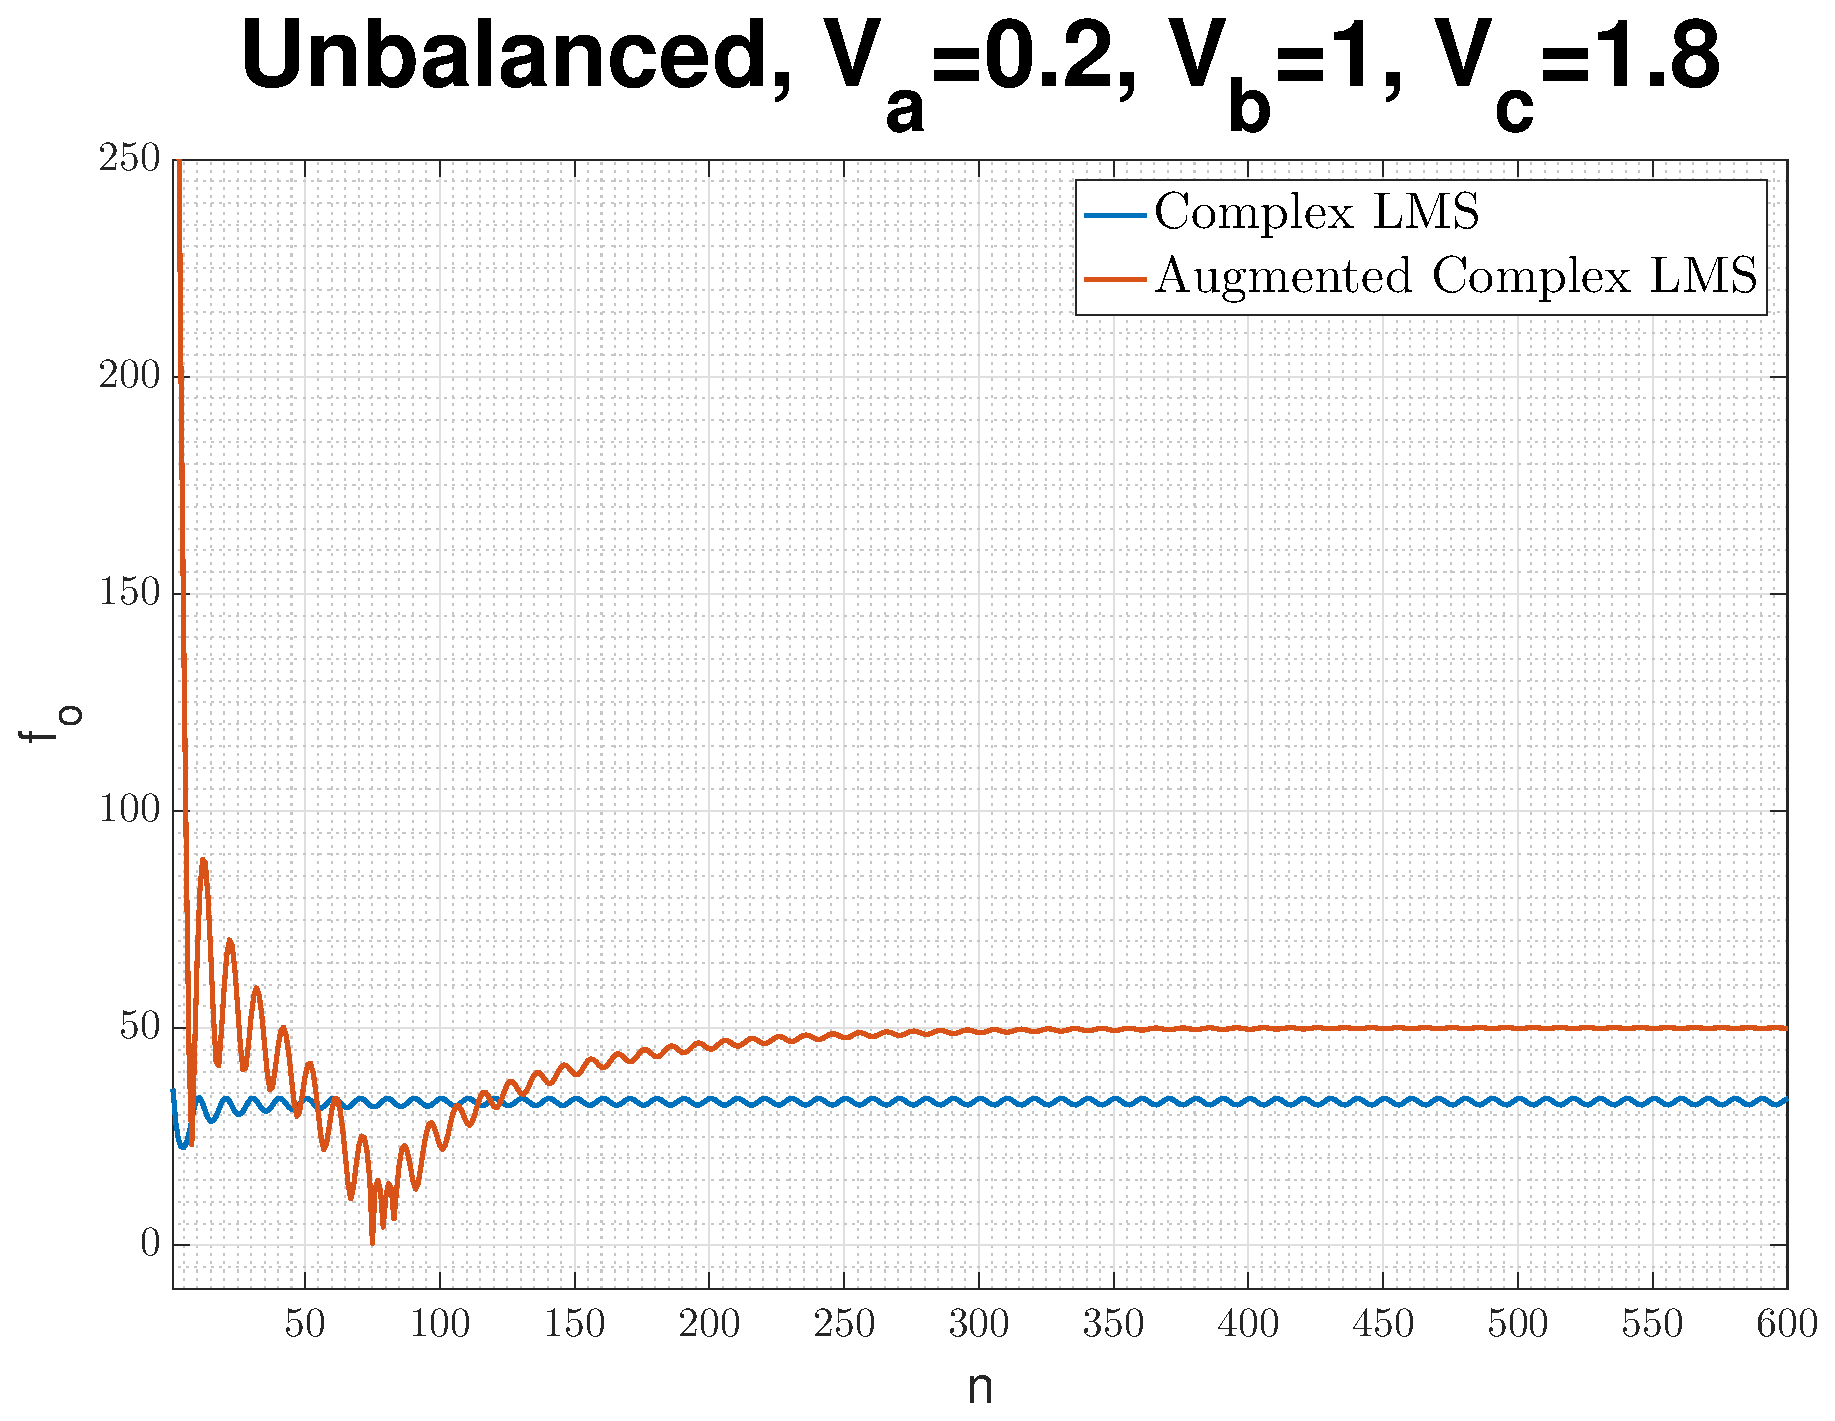
\includegraphics[width=0.32\textwidth]{part4/unbalanced_sys_clms_aclms_magnitude}
\caption{Comparison of CLMS and ACLMS for Unbalanced Complex Voltages}
\label{fig:unbalanced}
\end{figure}


\subsection{Adaptive AR Model Based Time-Frequency Estimation}

\noindent{}a. A frequency modulated signal is generated using circular white-gaussian noise with zero mean and variance of 0.05. The figure below shows that the signal's frequency is non-stationary. The figure also shows the frequency spectrum obtained if the entire signal is modeled as an AR process. Modeling the entire signal as an AR-process is not wise. The matlab function \texttt{aryule} assumes that the input signal is stationary. This is evidently not the case for this frequency modulated signal. The signal has 3 distinct stages in which the frequency is either constant, increasing linearly or increasing quadratically. It would be possible to performed block-based autoregressive modeling. If three blocks each of 500 samples were generated and run through \texttt{aryule}, we would be able to model the first block which has a constant frequency. The non-stationarity present in the other 2 blocks would still not be captured by the AR process. 

\begin{figure}[H]
\centering{}
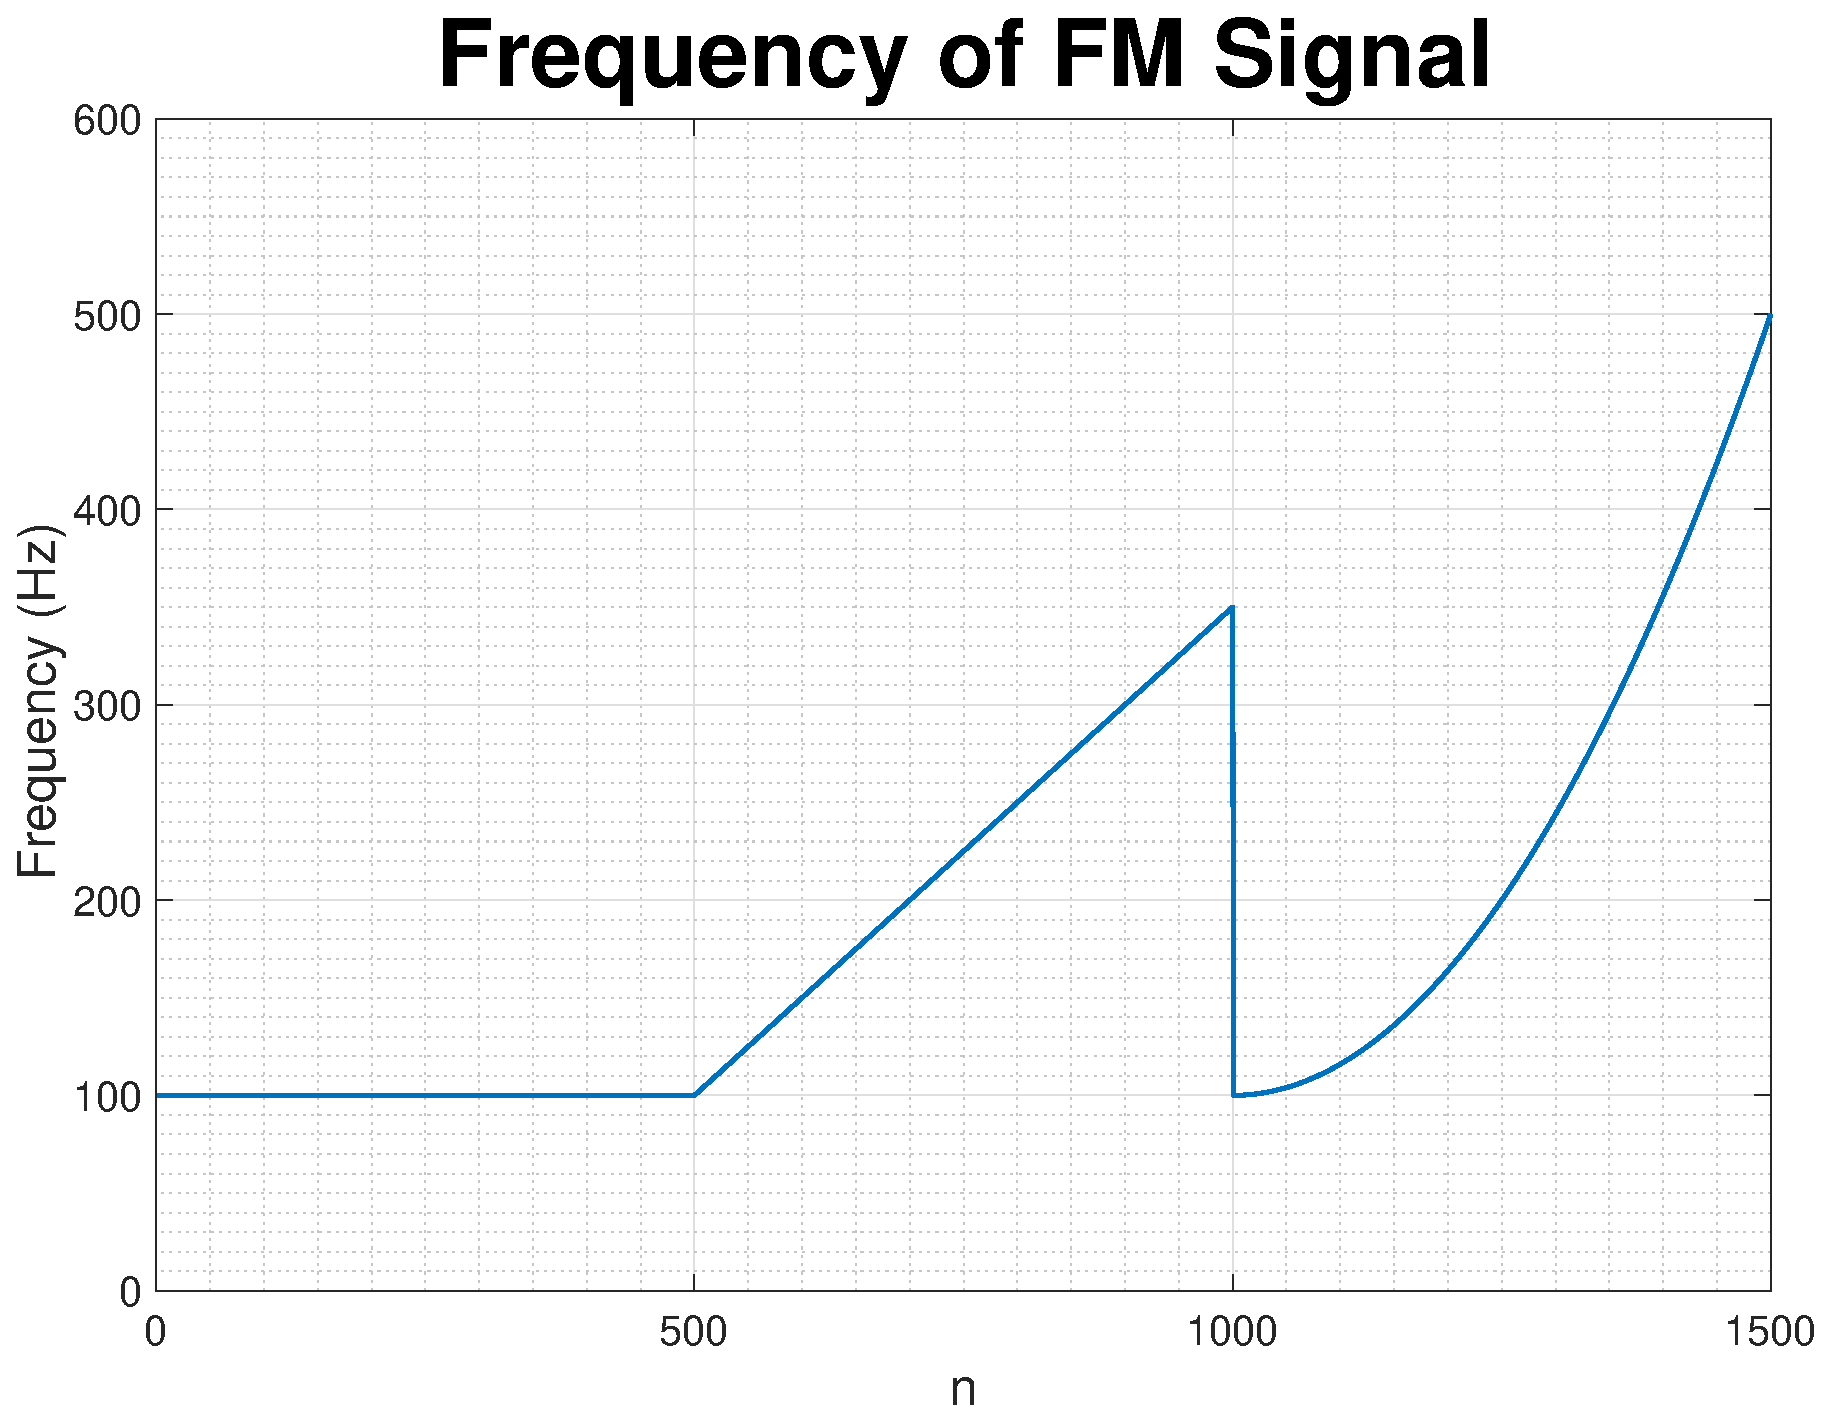
\includegraphics[width=0.32\textwidth]{part4/frequency_original_fm_signal}
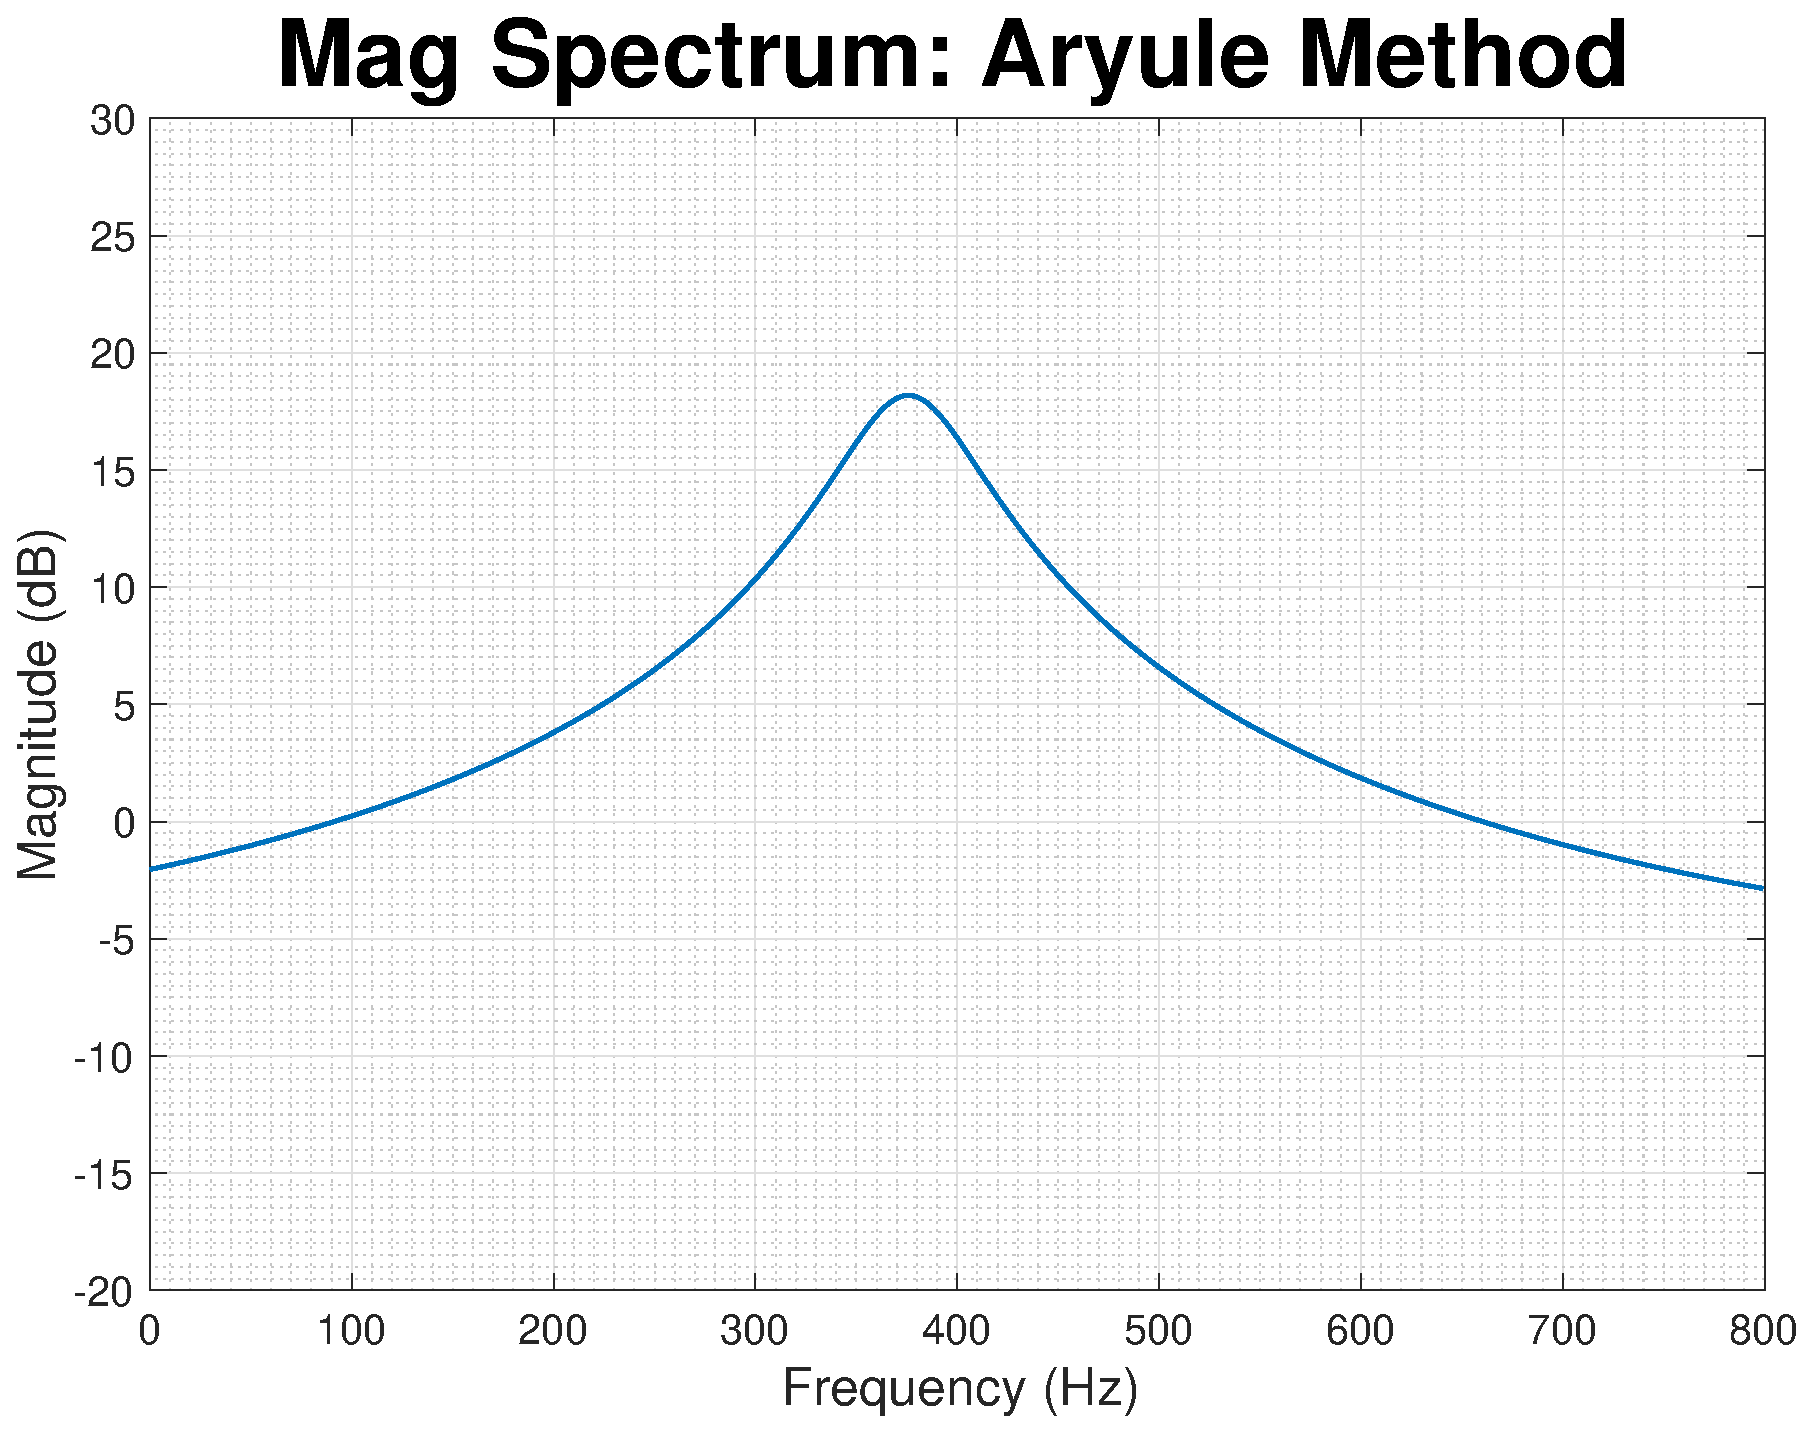
\includegraphics[width=0.32\textwidth]{part4/frequency_aryule_fm_signal}
\caption{Original, Non-Stationary Frequency of FM Signal and Power Spectrum obtained using Block-Based Estimate of AR Coefficients}
\end{figure}

\noindent{}b. Using the CLMS algorithm to infer the weights allows for us to capture the non-stationarity in the data. We are now optimizing the value of the AR coefficient in an adaptive manner rather than considering the entire dataset all at once. The figure below shows the results that are obtained. The impact that the choice of $\mu$ has is very clear. In the previous sections, the effect of $\mu$ on the rate of convergence was discussed at great length. The graphs below justify the need for fast convergence in a real-world application such as tracking the frequency of a signal. Notice that a large value of $\mu$ leads to a thicker yellow line. The thickness of the line indicates that there is a large variation in the exact frequency of the signal. Again this highlights the trade-off between convergence speed and steady state error.

\begin{figure}[H]
\centering{}
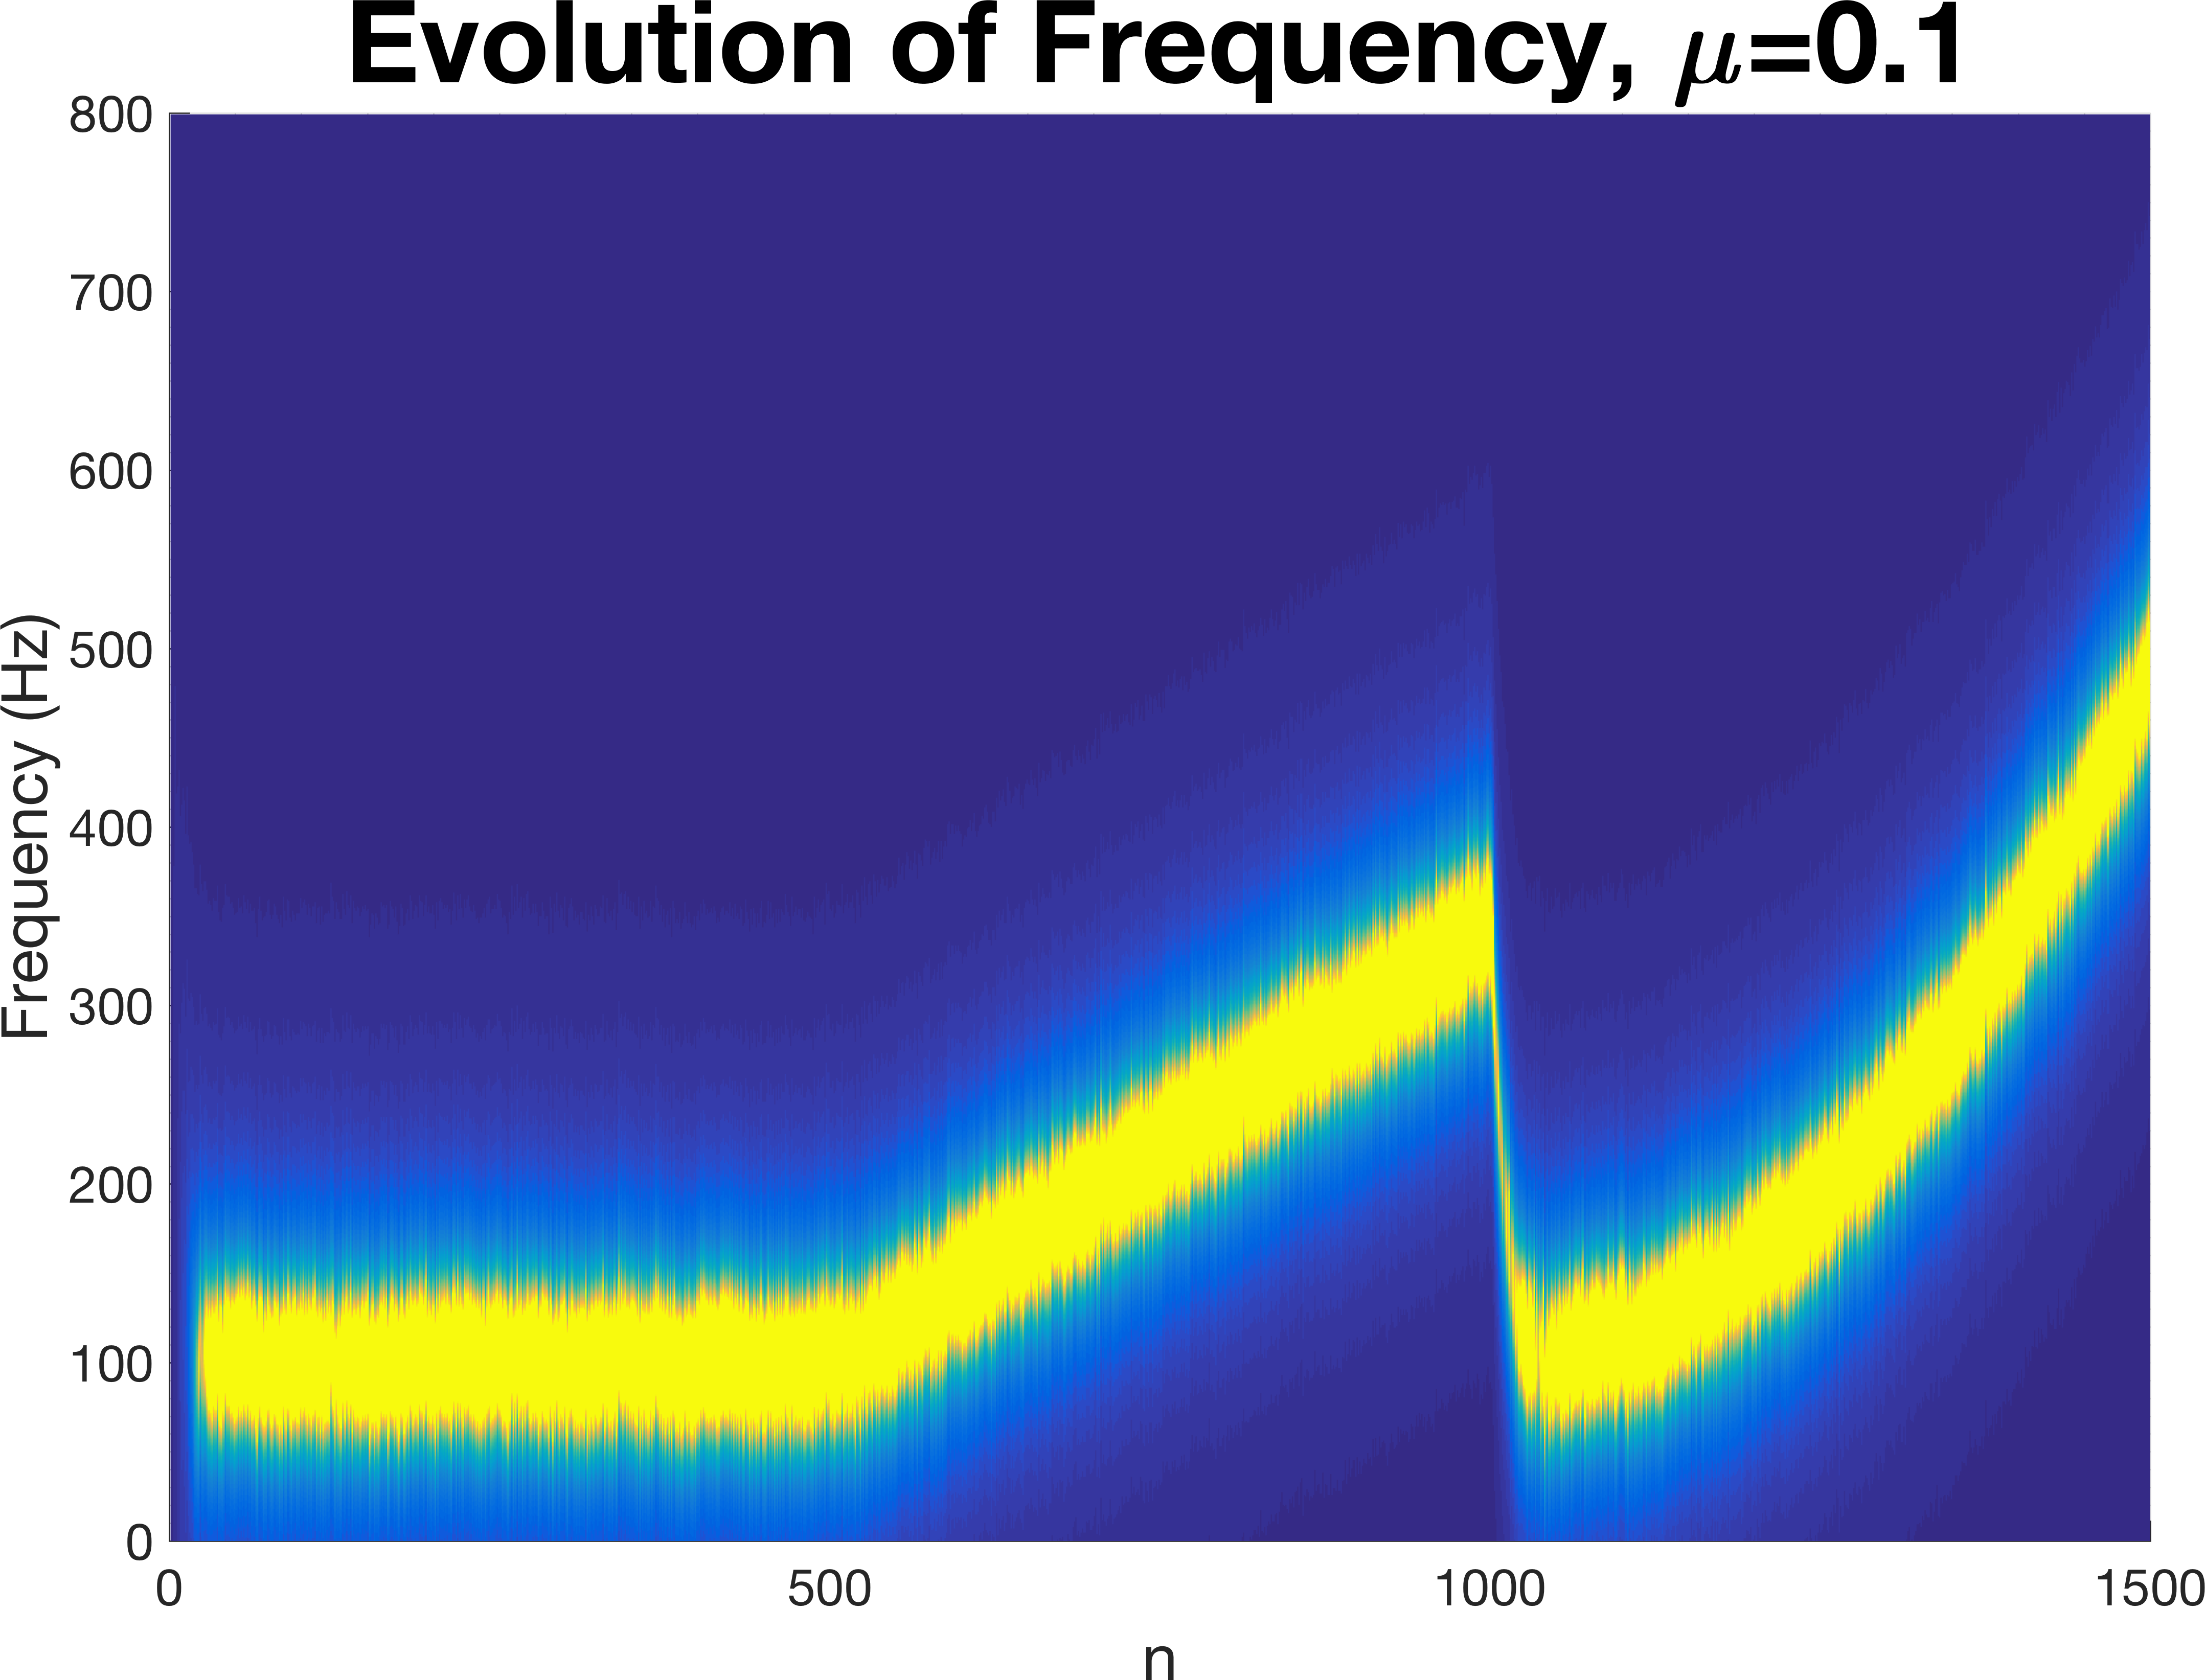
\includegraphics[width=0.32\textwidth]{part4/frequency_clms_fm_signal_1}
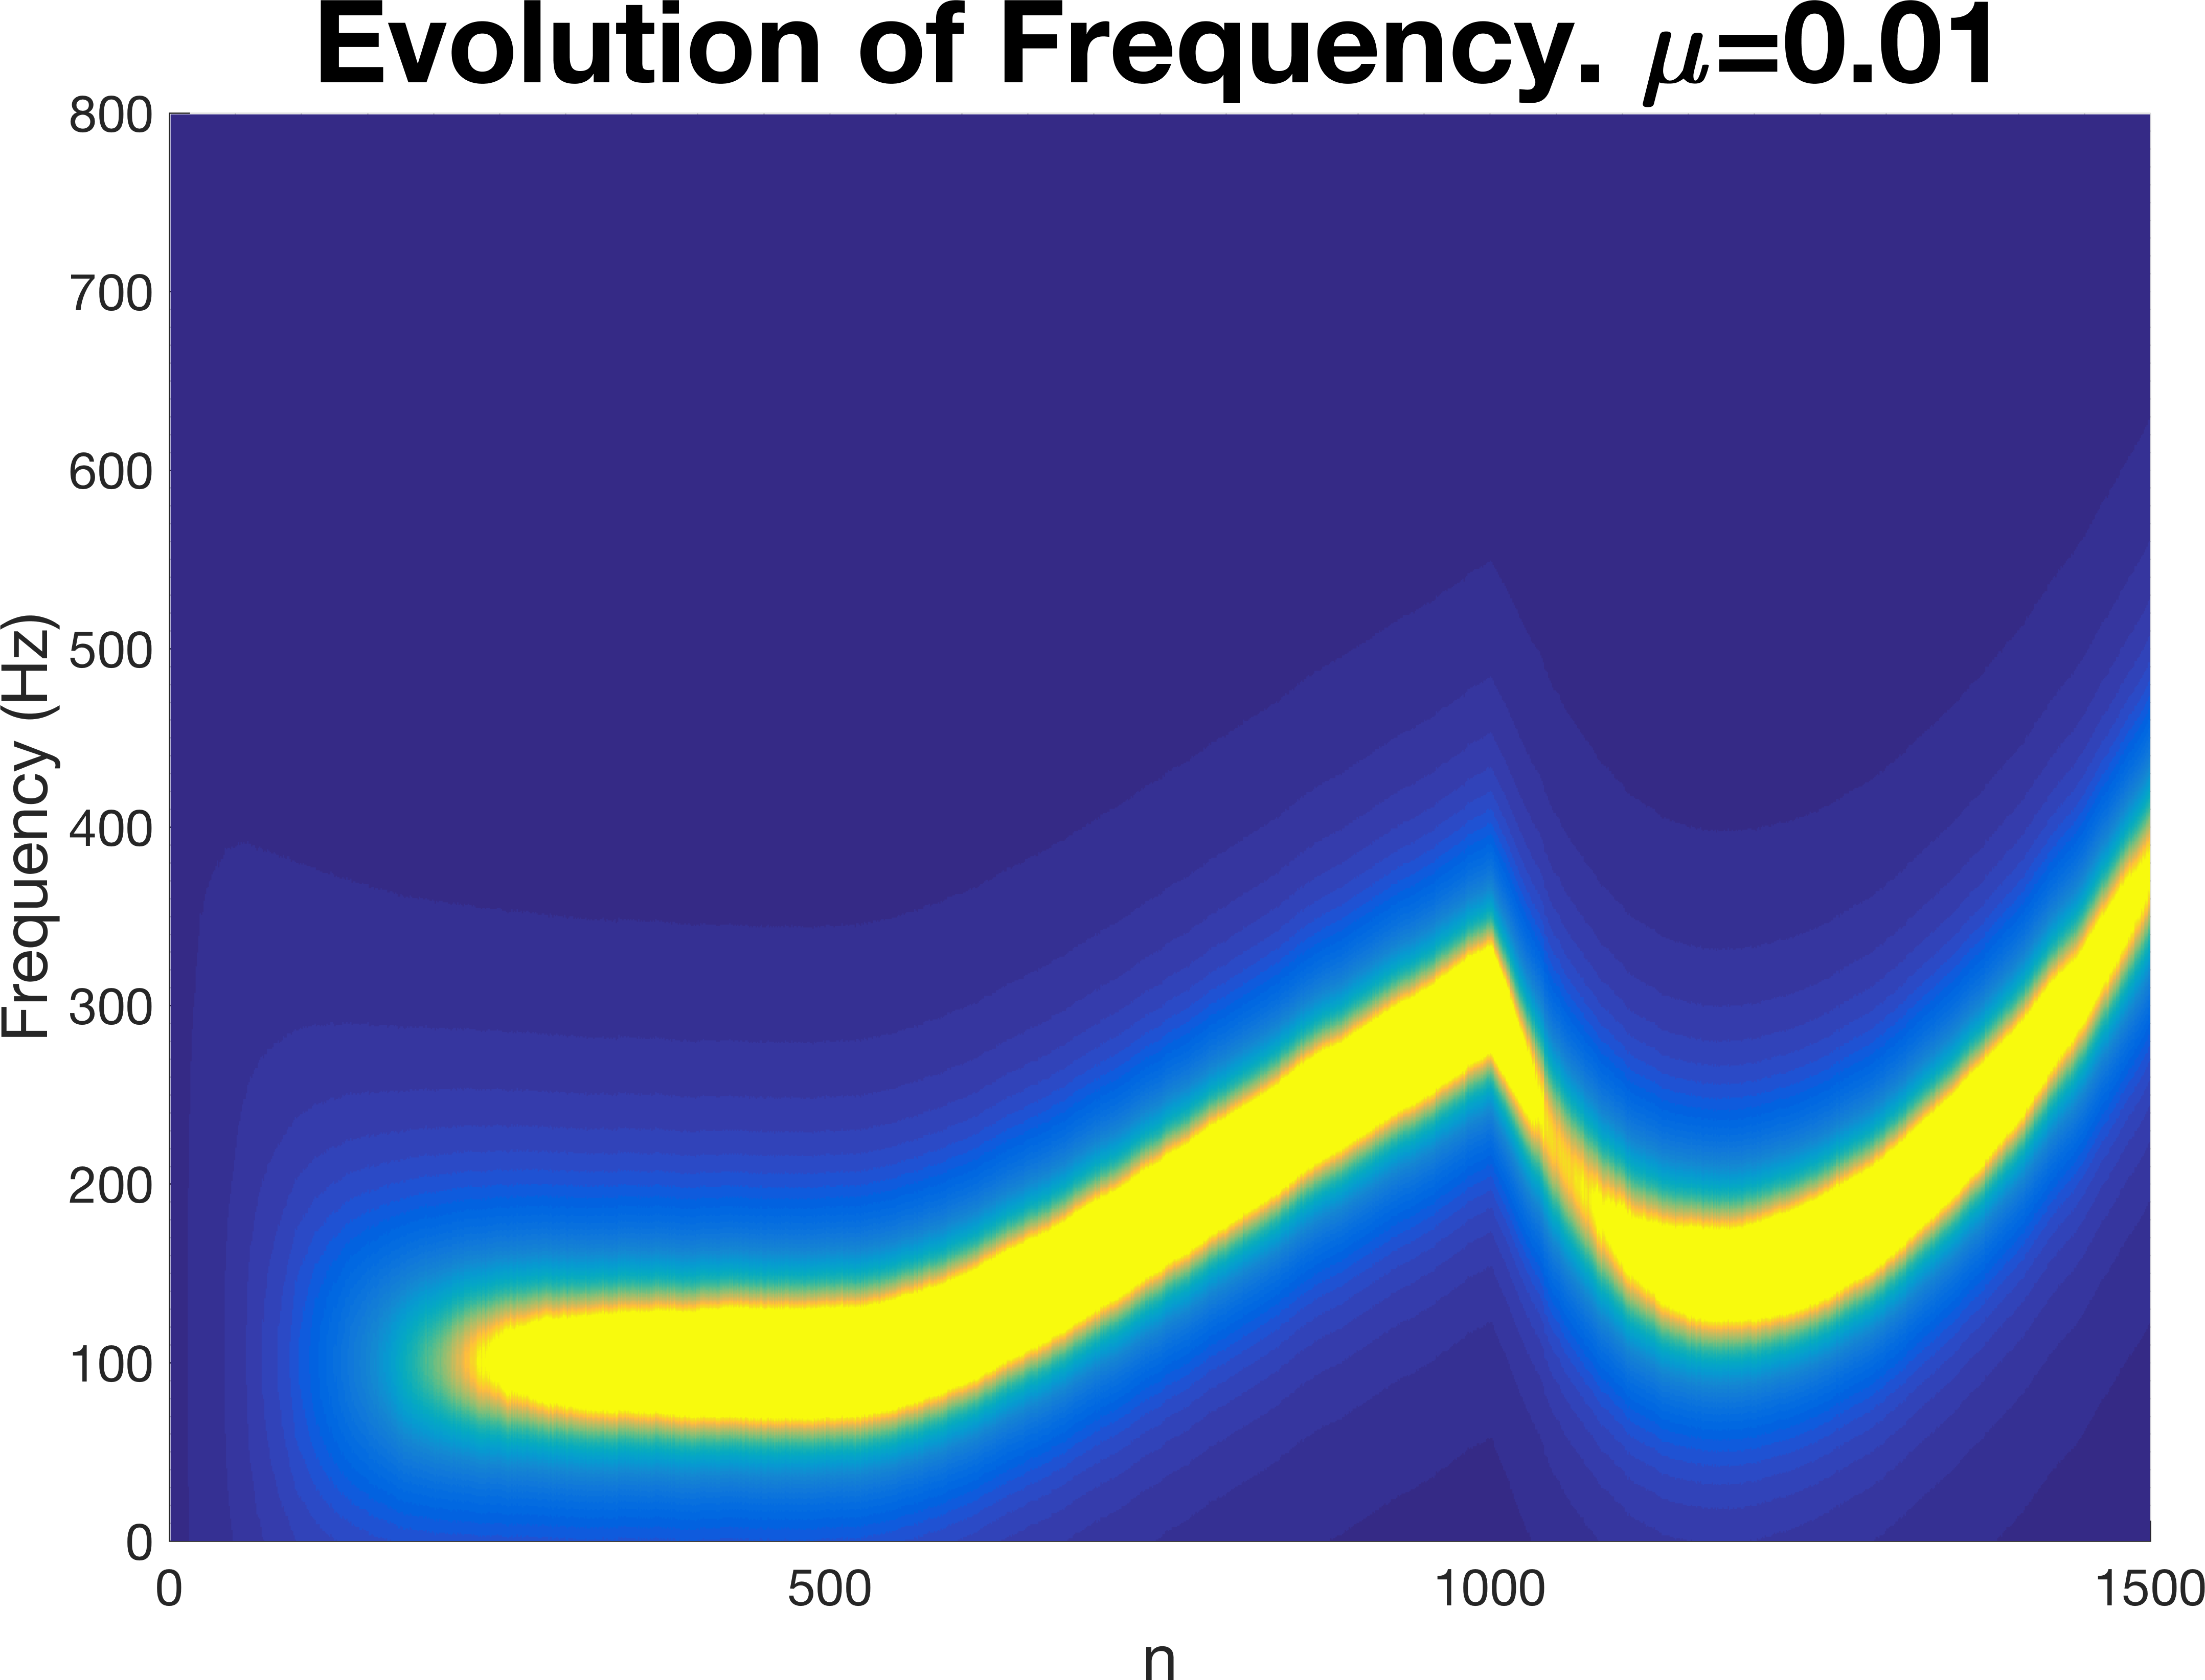
\includegraphics[width=0.32\textwidth]{part4/frequency_clms_fm_signal_01}
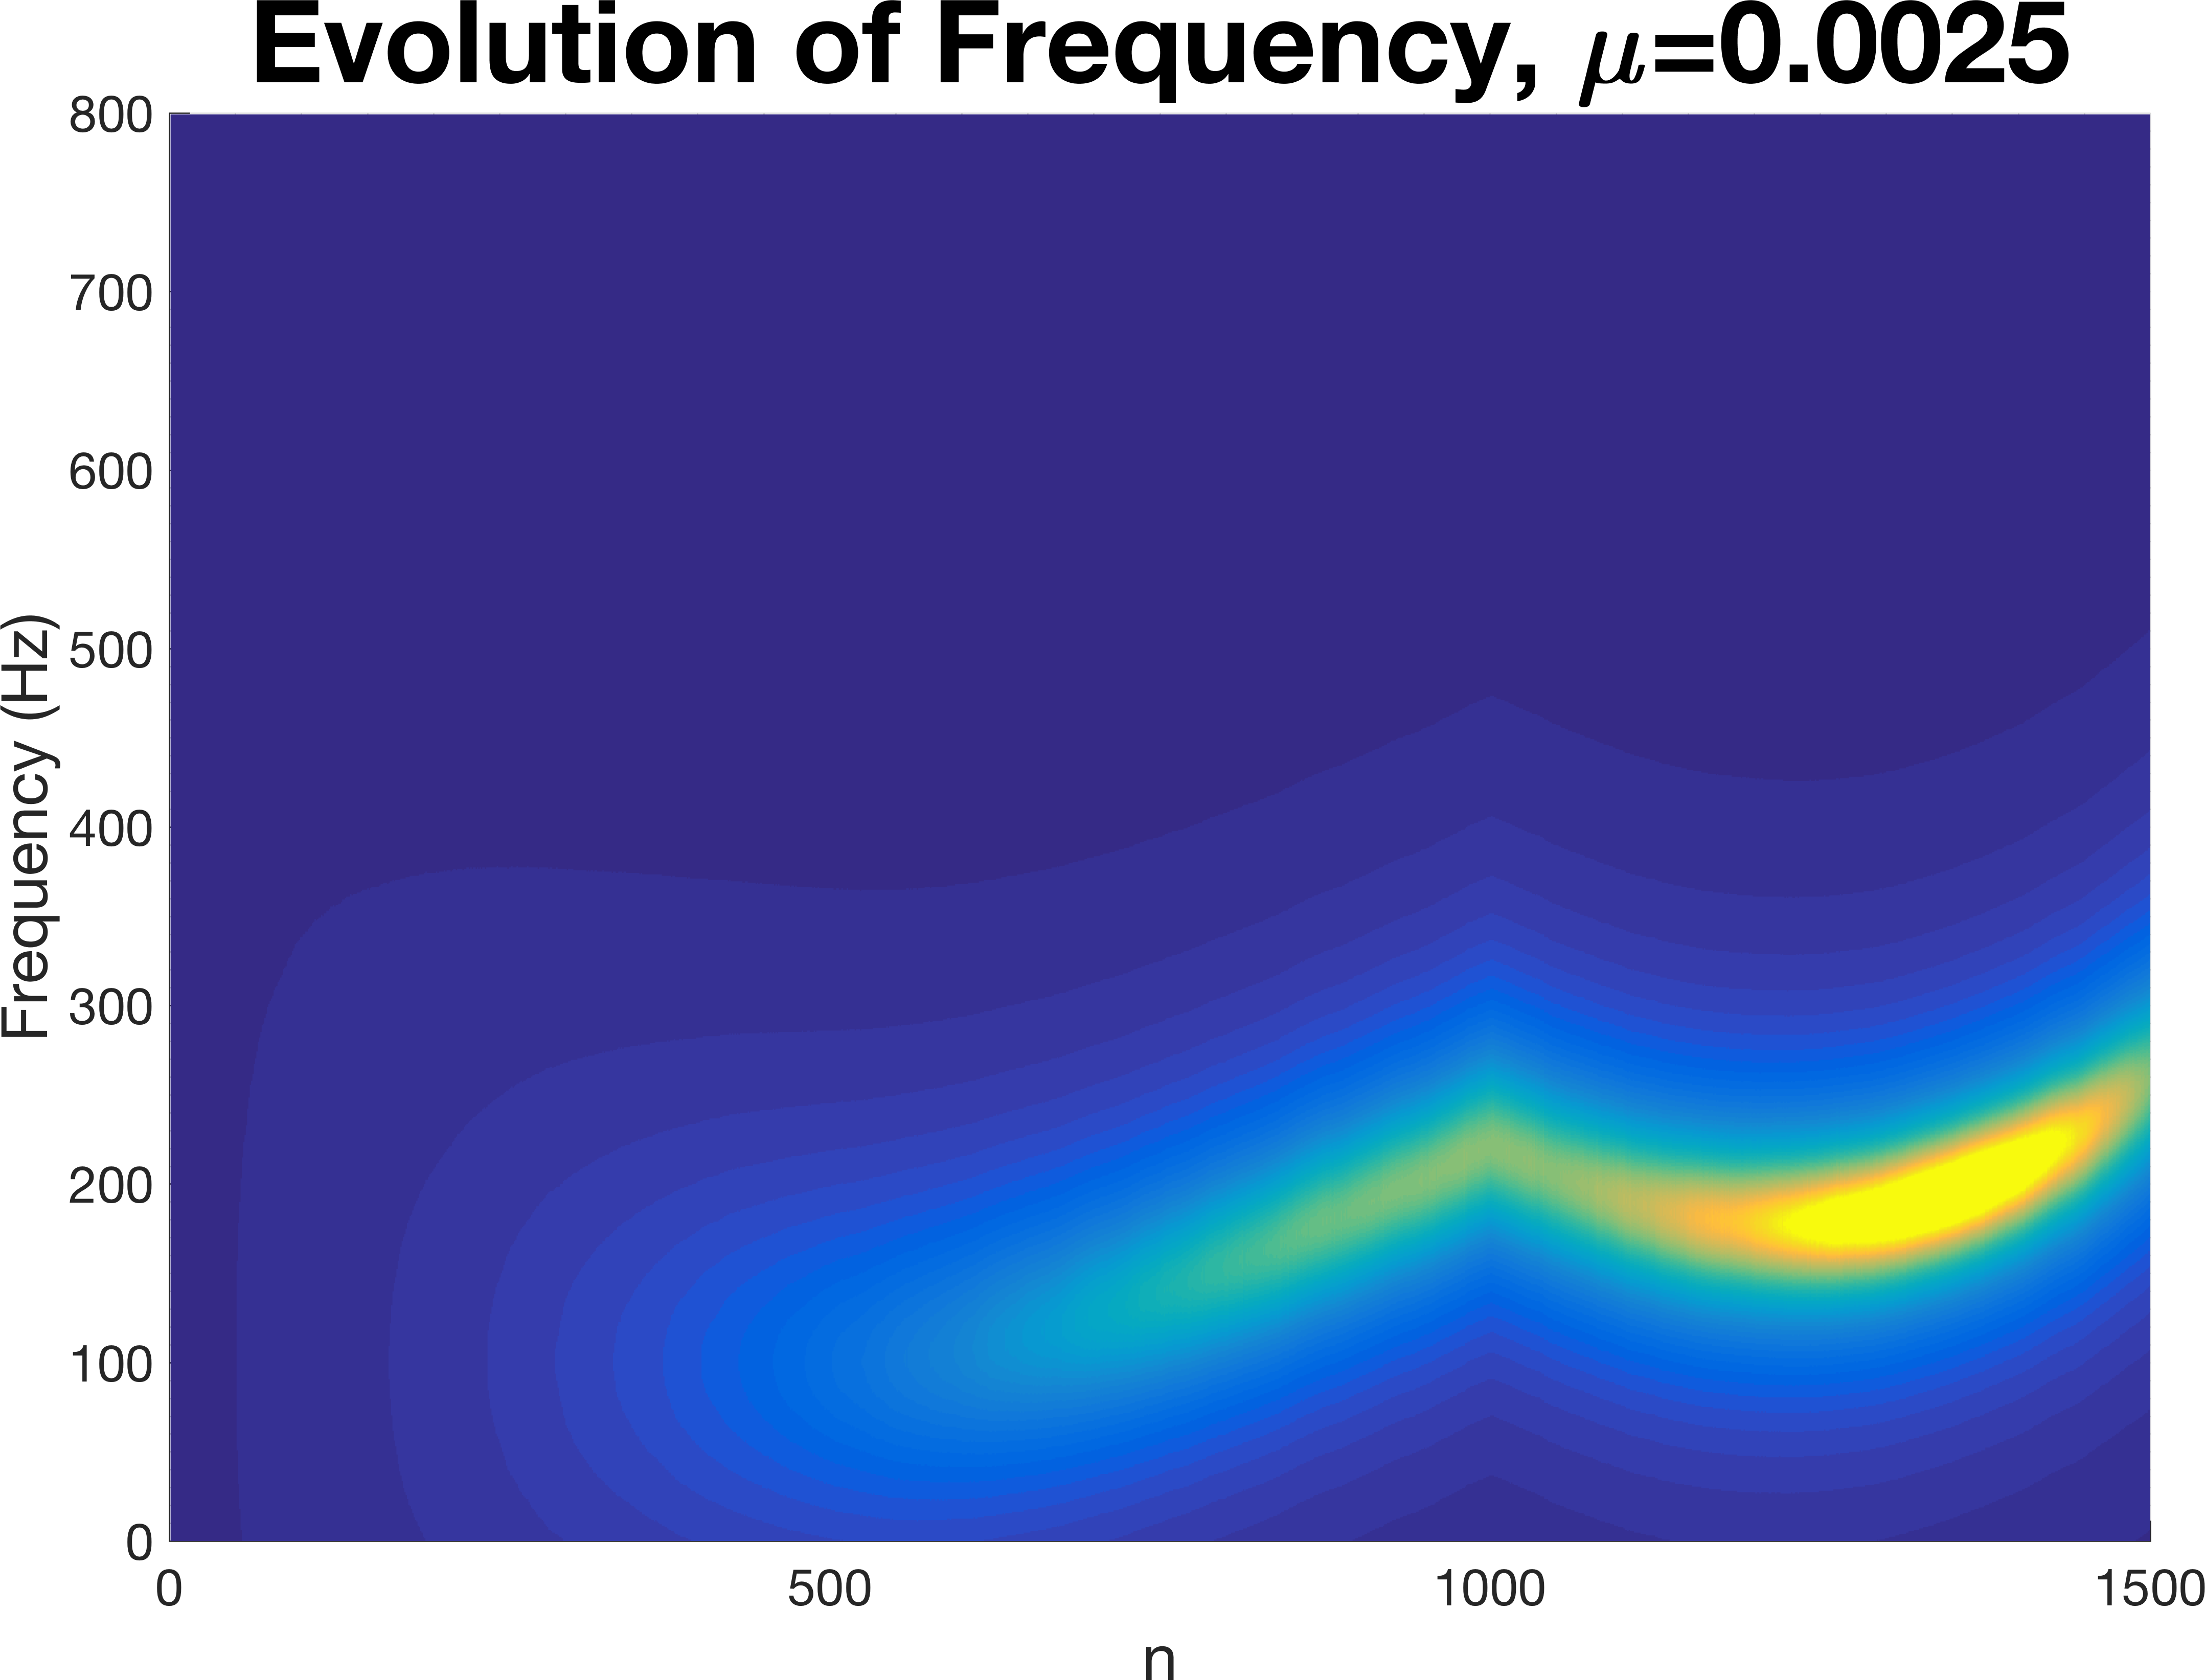
\includegraphics[width=0.32\textwidth]{part4/frequency_clms_fm_signal_0025}
\caption{Time-Frequency Estimation using Complex LMS Algorithm with Different Values of $\mu$}
\end{figure}

\subsection{A Real Time Spectrum Analyser Using Least Mean Square}

\noindent{}a. To solve the least squares problem, we start first with the cost function in (\ref{eq:ft_cost})

\begin{align}
\underset{\textbf{w}}{\text{min}} ||\textbf{y}-\hat{\textbf{y}}||^2 =  \underset{\textbf{w}}{\text{min}} \sum_{n=0}^{N-1}|y(n)-\hat{y}(n)|^2\label{eq:ft_cost}
\end{align}

\noindent{}We can start by expressing $||\textbf{y}-\hat{\textbf{y}}||^2$ as:

\begin{align*}
||\textbf{y}-\hat{\textbf{y}}||^2 &= (\textbf{y}-\hat{\textbf{y}})^H(\textbf{y}-\hat{\textbf{y}}) \\
&= (\textbf{y}-\textbf{F}\textbf{w})^H(\textbf{y}-\textbf{F}\textbf{w}) \\
&= \textbf{y}^H\textbf{y} - \textbf{w}^H\textbf{F}^H\textbf{y} - \textbf{y}^H\textbf{F}\textbf{w} + \textbf{w}^w\big(\textbf{F}^H\textbf{F}\big)\textbf{w}
\end{align*}

\noindent{}To minimize with respect to $\textbf{w}$, we differentiate the above equation with respect to $\textbf{w}$:

\begin{align*}
0 -\textbf{y}^H\textbf{F} - \textbf{y}^H\textbf{F} + \textbf{w}^H\big(\textbf{F}^H\textbf{F}+\textbf{F}^H\textbf{F}\big)
\end{align*}

\noindent{}Equating the derivative to 0, cancelling out the common terms and taking the transpose on each side, we get:

\begin{align*}
-\textbf{y}^H\textbf{F} - \textbf{y}^H\textbf{F} + \textbf{w}\big(\textbf{F}^H\textbf{F}+\textbf{F}^H\textbf{F}\big) &= 0 \\
2 \textbf{w}^H\textbf{F}^H\textbf{F} &= 2\textbf{y}^H\textbf{F}^H\\
\textbf{F}^H\textbf{F} \textbf{w} &= \textbf{F}\textbf{y}
\end{align*}

\noindent{}Inverting the matrix $\textbf{F}^H\textbf{F}$ gives (\ref{eq:ft_proof}) which completes the proof:

\begin{align}
\textbf{w} = \big(\textbf{F}^H\textbf{F}\big)^{-1} \textbf{F}\textbf{y} \label{eq:ft_proof}
\end{align}

\noindent{}We know that the Inverse Discrete Fourier Transform (DFT), for a signal $\hat{x}(n)$, is given by the equation in (\ref{eq:dft_formula}):

\begin{align}
\hat{x}(n) = \frac{1}{N} \sum_{k=0}^{N-1}X(K)e^{j2\pi n k / N} \label{eq:dft_formula}
\end{align}

\noindent{}The formula in (\ref{eq:dft_formula}) can easily be express in the following matrix vector notation, where $W_{n,k}=e^{j2\pi n k / N}$:

\begin{align*}
\begin{bmatrix}
\hat{x}(0) \\
\hat{x}(1) \\
\vdots\\
\hat{x}(N-1)
\end{bmatrix}
&=
\begin{bmatrix}
    W_{0,0}		& W_{0,1} 	& \dots	& W_{0,N-1} \\
    W_{1,0} 		& \ddots  	&		& \vdots		\\
   	\vdots		& 			& \ddots	& \vdots		\\
   	W_{N-1,0} 	& \dots 		& \dots	& W_{N-1,N-1}
\end{bmatrix} 
\begin{bmatrix}
X(0) \\
X(1) \\
\vdots \\
X(N-1)
\end{bmatrix}
\end{align*}

\noindent{}In compact notation, 

\begin{align*}
\hat{\textbf{x}} &= \textbf{W}\textbf{X}
\end{align*}

\noindent{}Using the matrix vector form of the Inverse DFT, it is clear that the Fourier Coefficients, $\textbf{X}$, can be determined using the formula derived in (\ref{eq:ft_proof}), which is reproduced below:

\begin{align}
\textbf{X} = \big(\textbf{W}^H\textbf{W}\big)^{-1} \textbf{W}\textbf{x}\label{eq:dft_inverse_form}
\end{align}
 
\noindent{}The Fourier coefficients, $\textbf{X}$, that (\ref{eq:dft_inverse_form}) returns would allow us to form a signal $\hat{\textbf{x}}$ such that the squared error between $\textbf{x}$ and $\hat{\textbf{x}}$ is minimized.\\

\noindent{}b. Using the matrix vector form of the Inverse DFT, it is clear that $\hat{\textbf{x}} = \textbf{W}\textbf{X}$ is an approximation of the signal $\textbf{x}$. The approximation comes from the fact that $\textbf{X}$ was formed by projecting $\textbf{x}$ onto the column space of $\textbf{W}$. Notice that the columns of $\textbf{W}$ form an orthonormal basis consisting of complex exponentials. In contrast to the Continuous Time Fourier Transform, the DFT only requires a finite set of basis vectors, namely $N$ for a signal $x(n)$ that has $N$ non-zero components. Notice that since we are projecting onto an orthonormal basis, Parseval's theorem will hold. Parseval's theorem would not hold if the basis that the signal $x(n)$ is projected on is not orthorgonal.\\

\noindent{}c. The DFT-CLMS algorithm is applied to the Frequency Modulated signal and the results obtained are shown in the figure below. The rough shape of the spectrum observed somewhat matches the ideal frequency spectrum. However, it seems that frequency components are everlasting. Once the algorithm picks up a frequency component, that frequency component forever remains in the spectrum. In actual fact, this comes about from the fact that the weights are updated in an adaptive manner rather than the weights being calculated at each time-instance. As such, for a frequency component to be removed from the spectrum, an error needs to be propogated back. This propogation of error takes some time and thus the frequency components seem to be everlasting.
 
\begin{figure}[H]
\centering{}
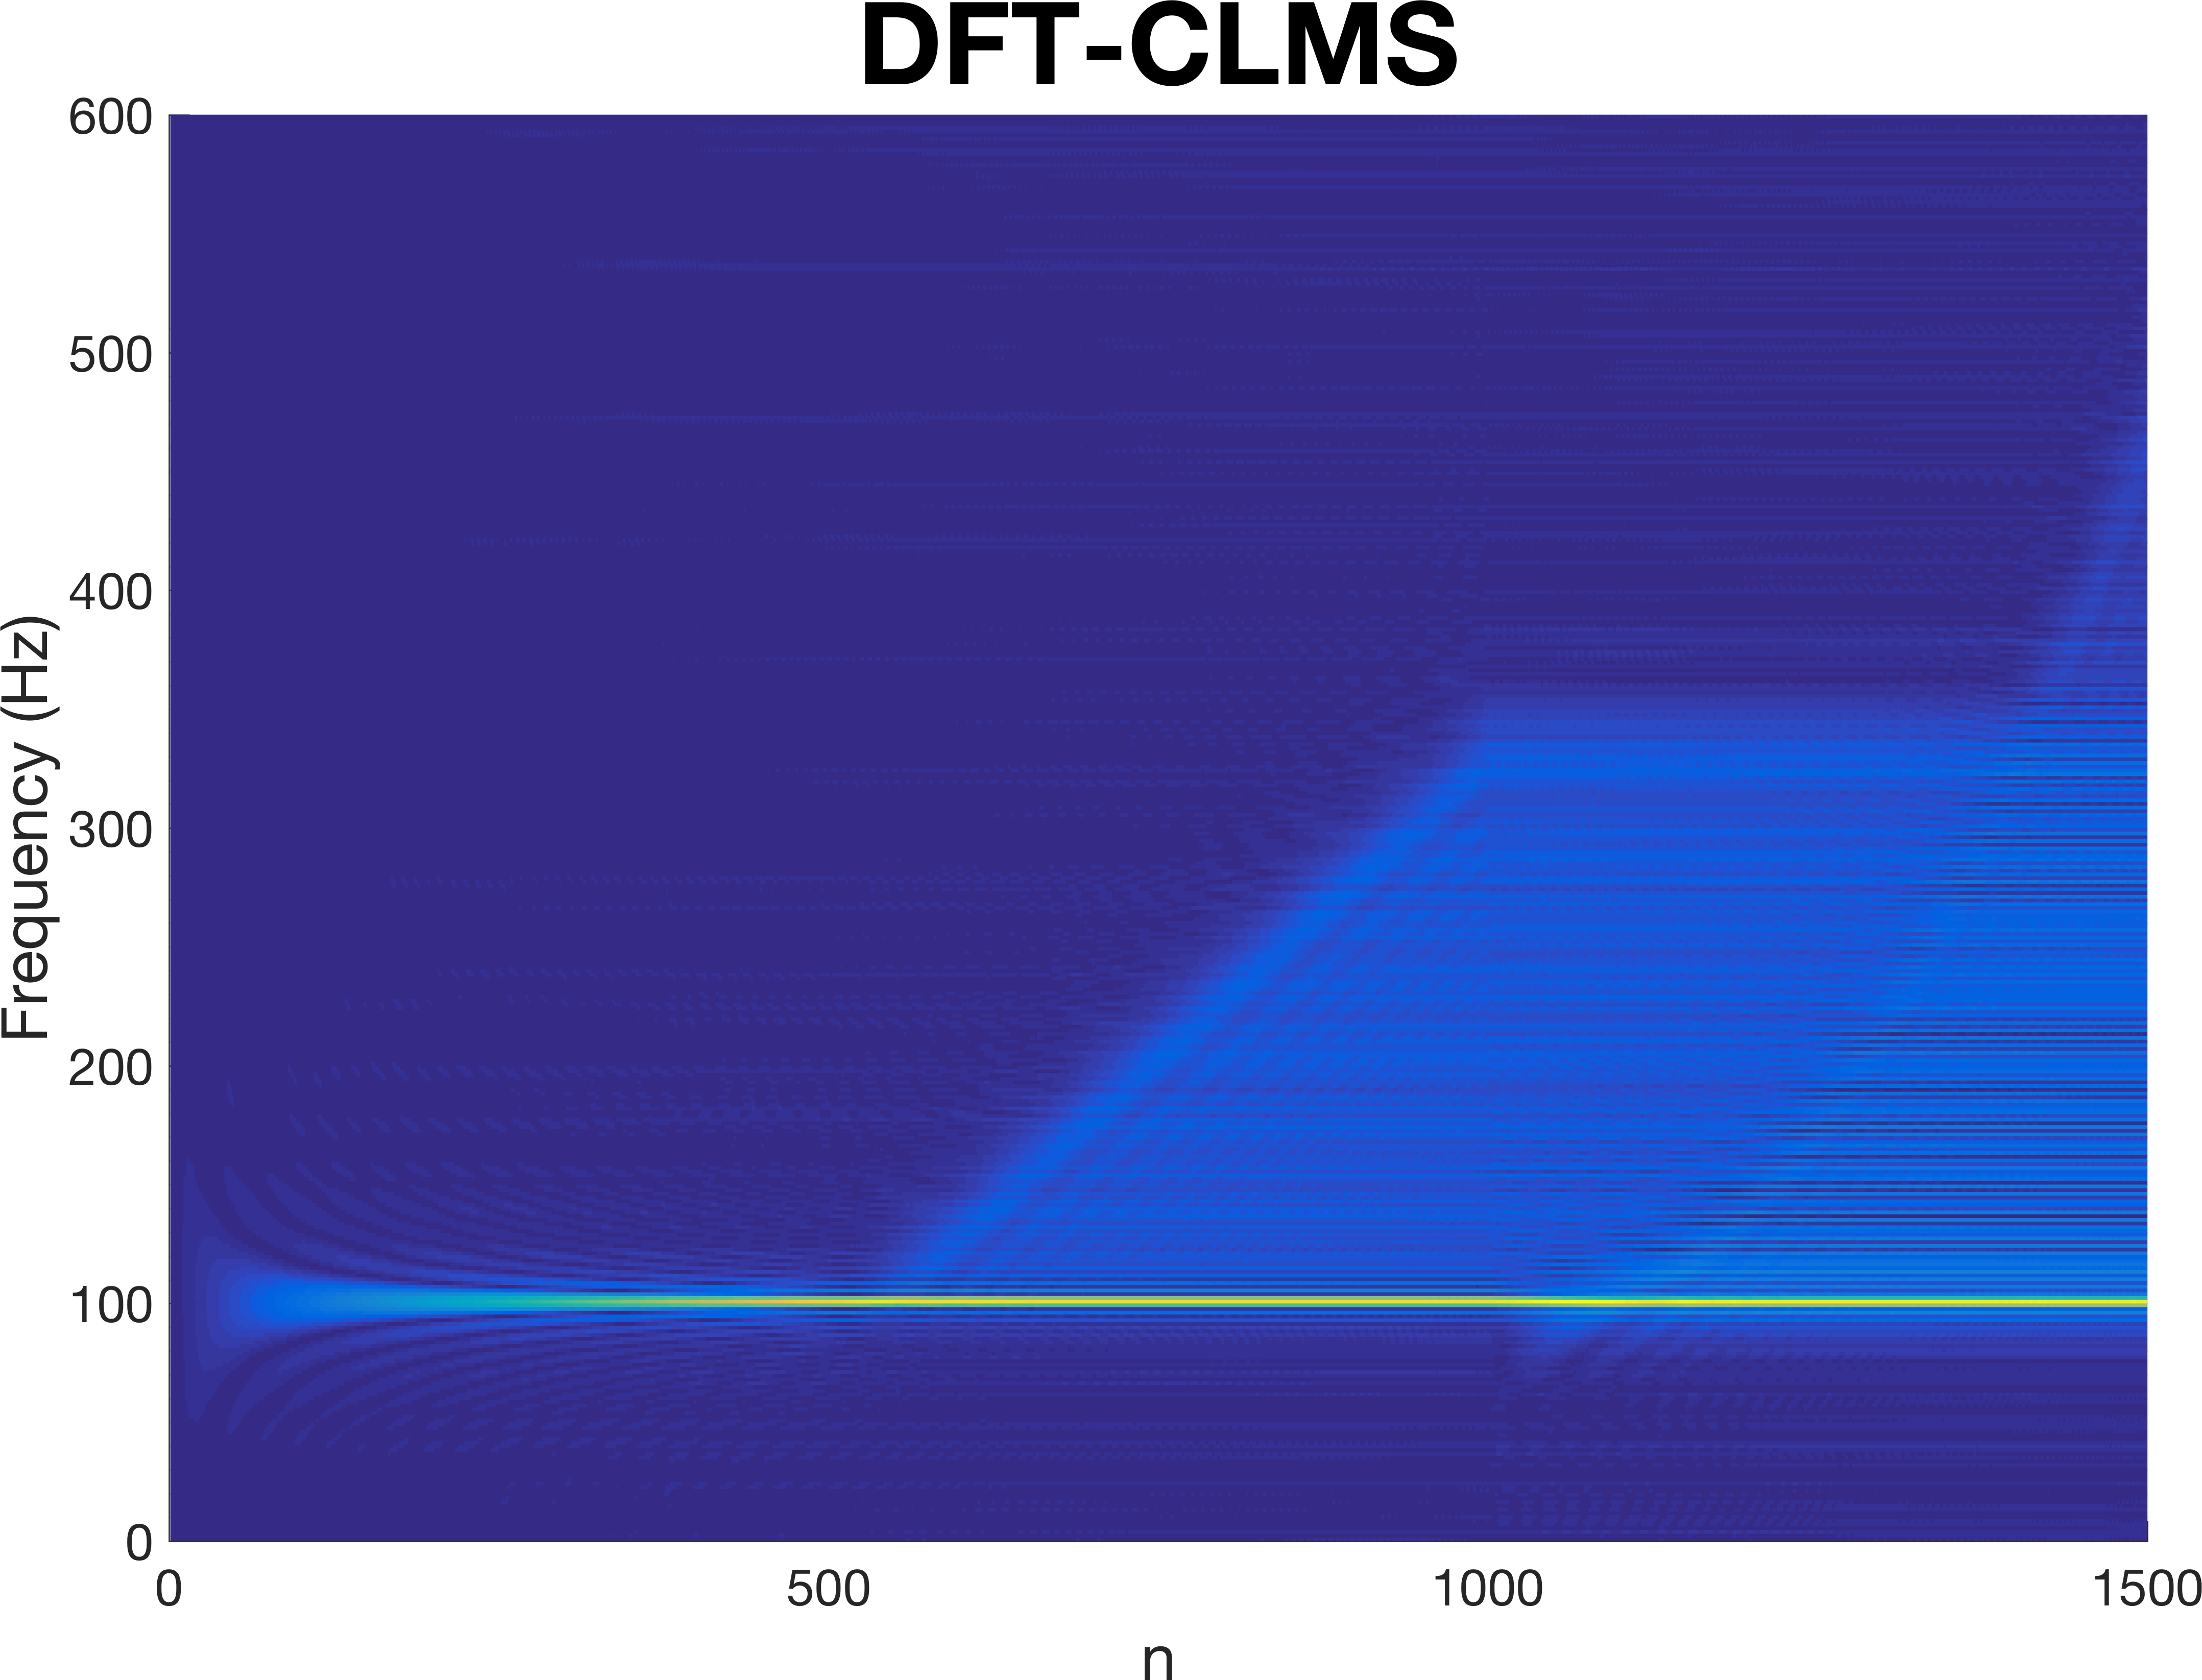
\includegraphics[width=0.32\textwidth]{part4/time_frequency_dft_non_leaky}
\caption{Time-Frequency Estimation using DFT-CLMS}
\end{figure}

\noindent{}To combat the slow trickle down effect that the error has, the Leaky-LMS algorithm is used instead. This allows the weights to be 'forgotten' and thus leads to a more accurate prediction of the weights. The value of $\gamma$ was set at $0.05$. The results obtained are significantly better. Notice that even such a small value of $0.05$ was able have a tremendous effect on the accuracy of the weights. Increasing the value of $\gamma$ beyond $0.05$ did not prove useful; the spectrum is would being estimated using very few values of signal and the dominant frequency tones would be correctly identified. 

\begin{figure}[H]
\centering{}
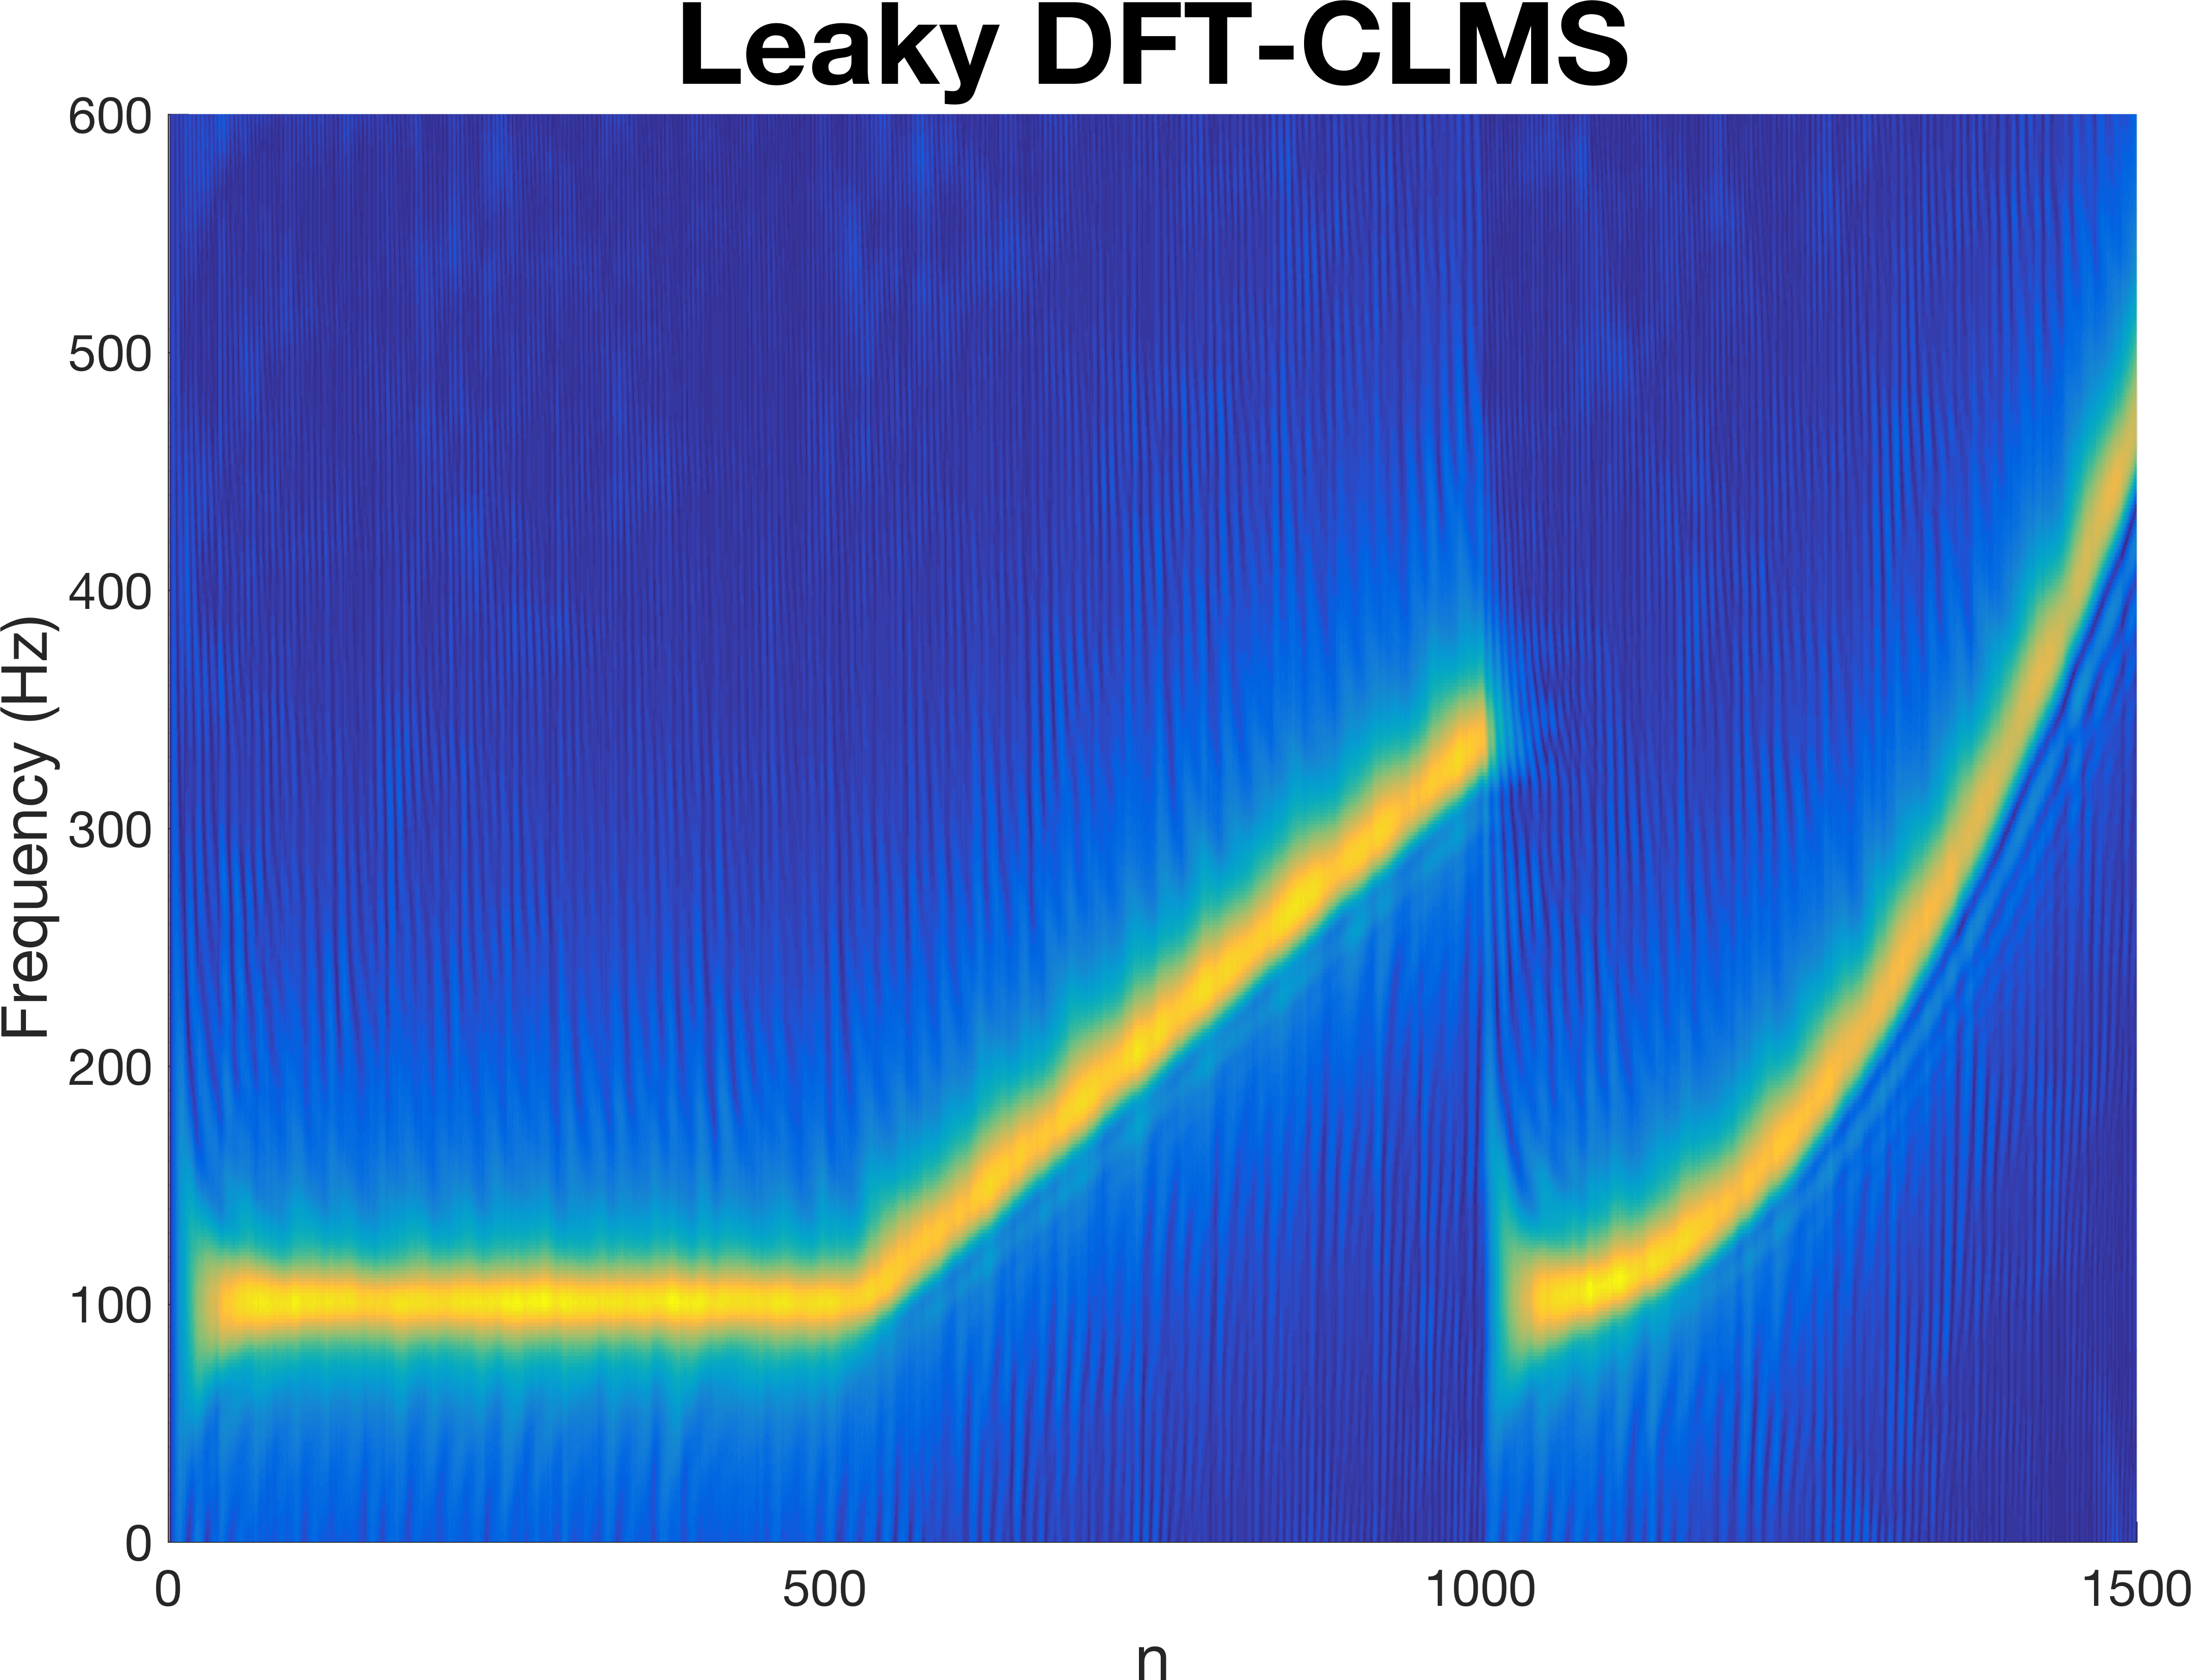
\includegraphics[width=0.32\textwidth]{part4/time_frequency_dft_leaky}
\caption{Time-Frequency Estimation using Leaky DFT-CLMS}
\end{figure}

\noindent{}d. The DFT-CLMS and Leaky DFT-CLMS algorithms are used to identify the spectrum of the EEG signal obtained from the POz location on the scalp. Both algorithm have identified clearly the strong component at 50 Hz. The first and second harmonics of the SSEVP have also been clearly identified at 13 Hz and 26 Hz. The third harmonic at 39 Hz is however indistinguishable. Notice that the Leaky DFT-CLMS algorithm does not work as well as the DFT-CLMS algorithm in this scenario. The reason for this is due to the stationary nature of the EEG signal. The Leaky DFT-CLMS, to some extent, 'forgets' weights that it learns. This amplifies the effect of placing a greater emphasis on recent samples rather than samples that were observed a very long time ago.  In so doing, it takes slightly longer to converge to a solution if the signal is stationary as in this case. The DFT-CLMS algorithm only 'forgets' weights using the backward error propagation mechanism and thus, in this case, is able to converge fast. Not only does the DFT-CLMS algorithm converge faster, it's ability to distinguish resonant components at 13, 26 and 50 Hz is also stronger; notice the brightness of the spectrogram at this frequencies. 

\begin{figure}[H]
\centering{}
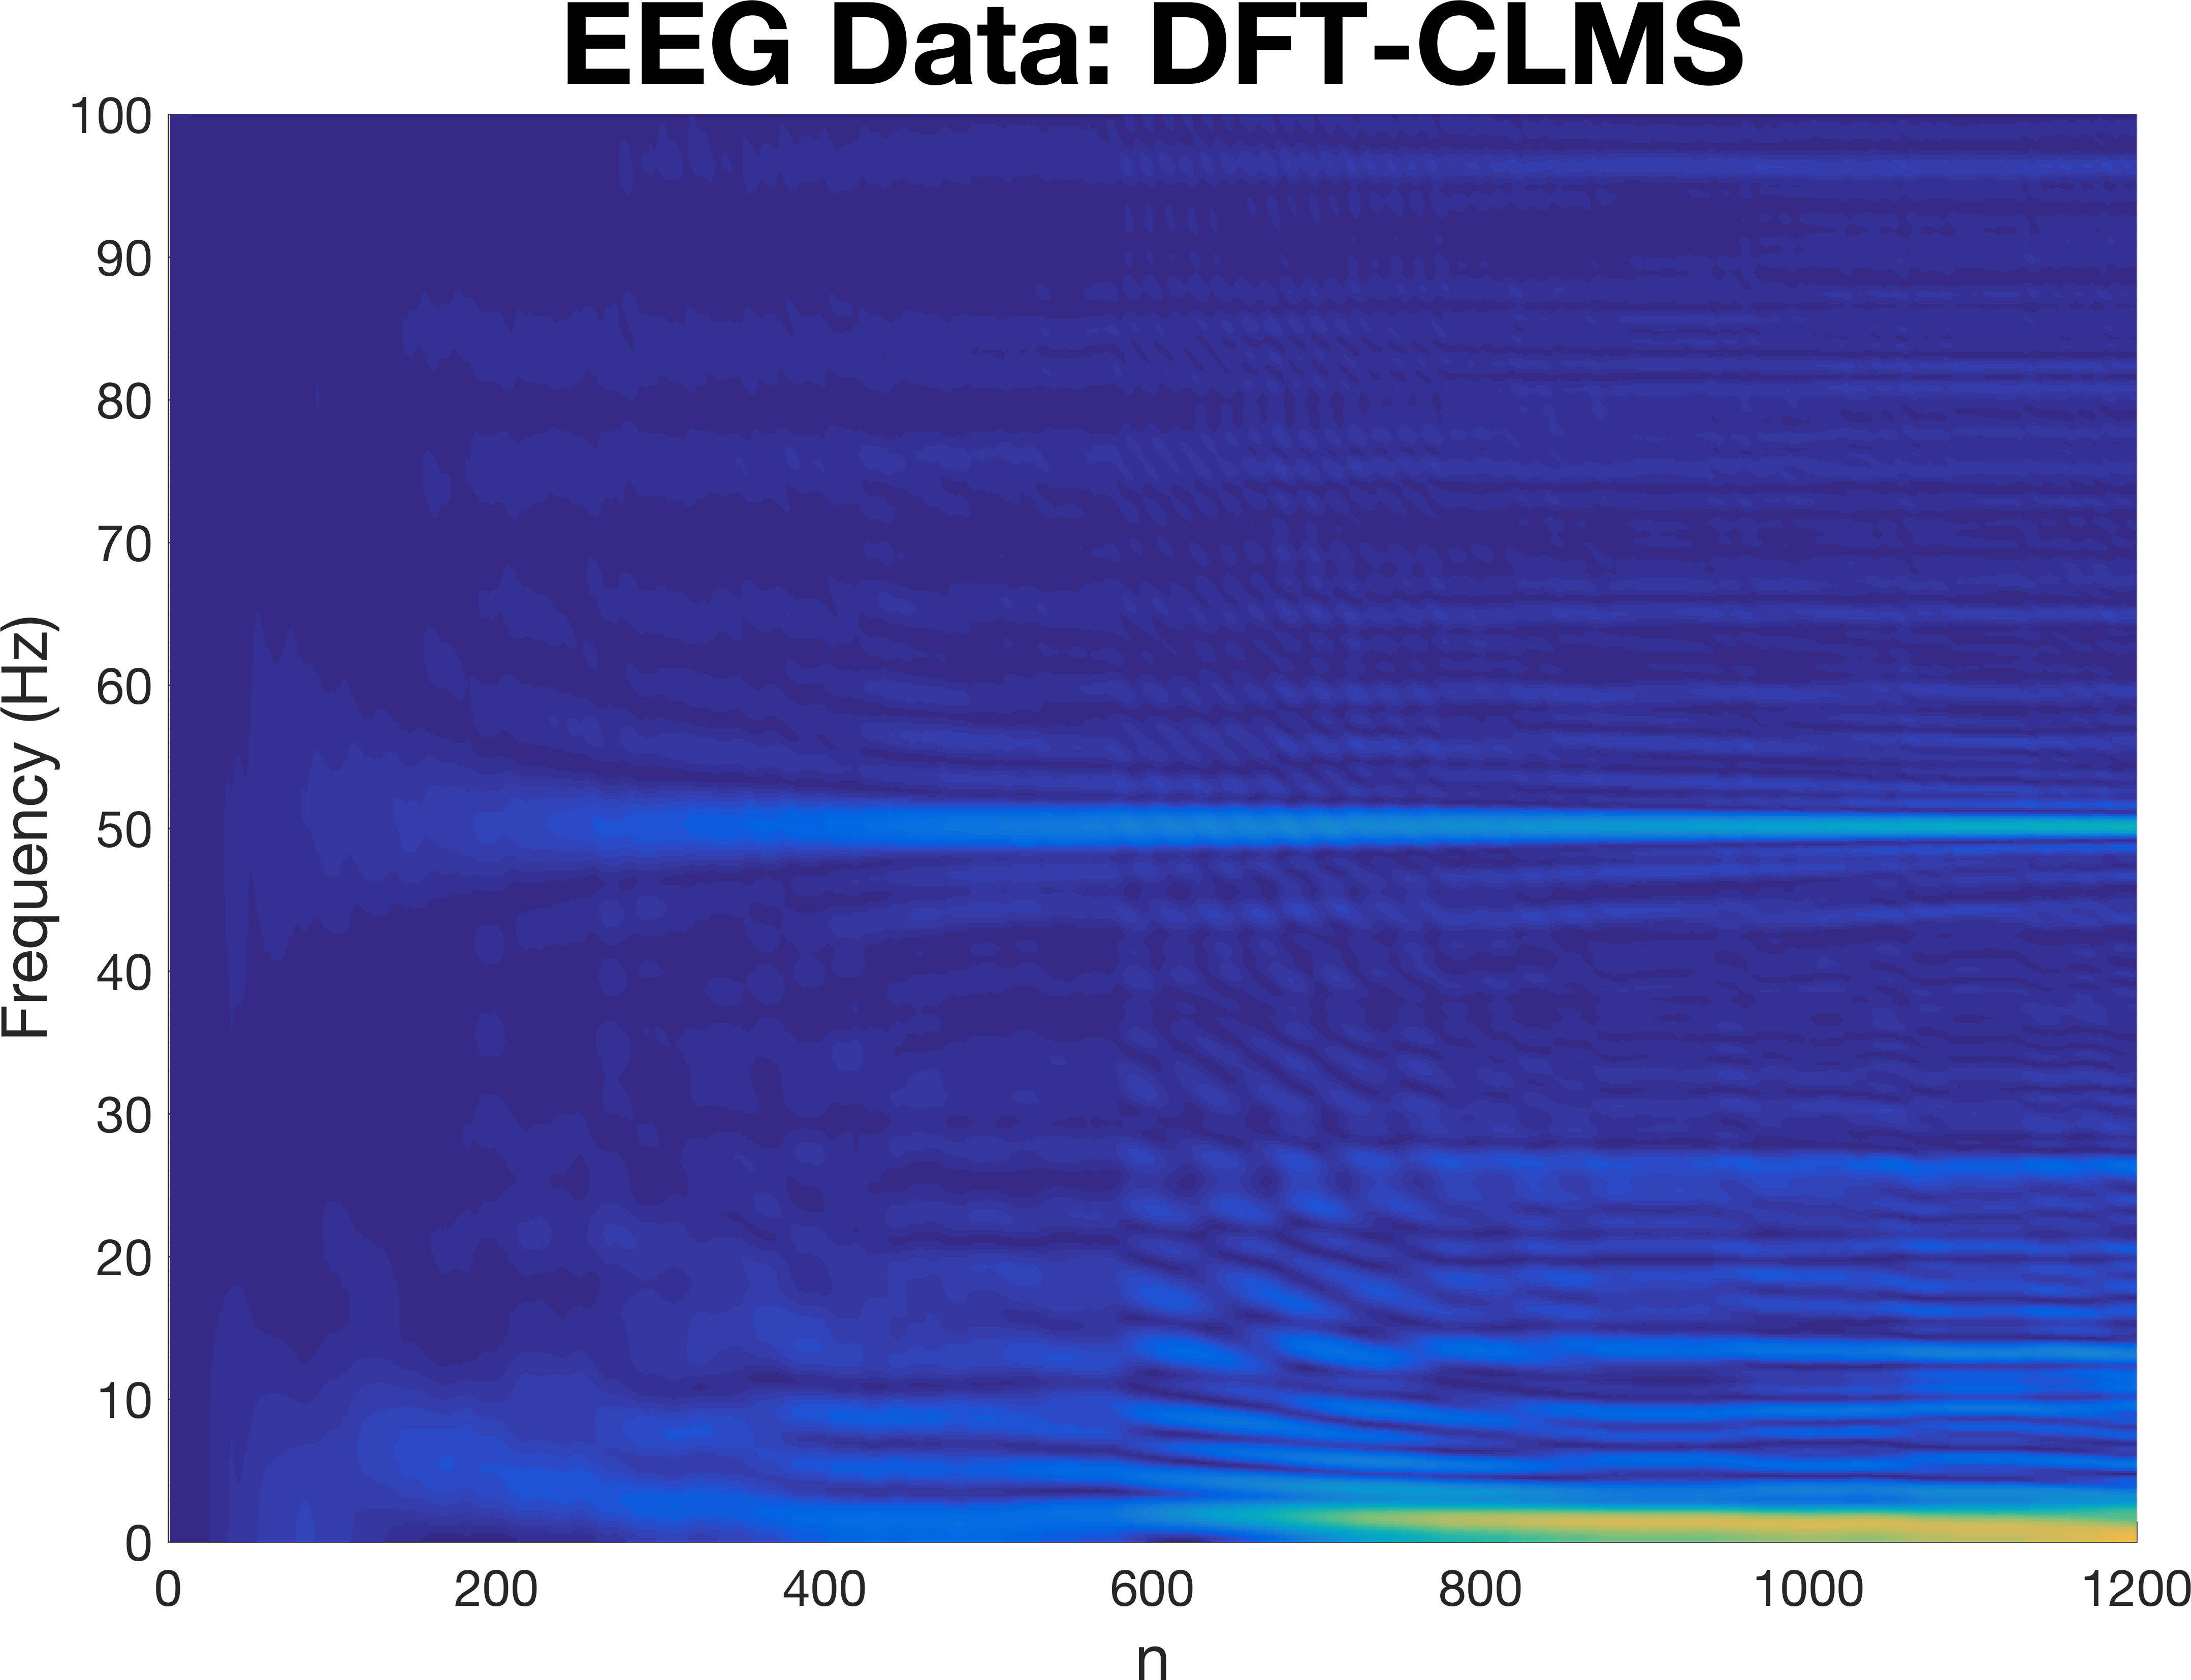
\includegraphics[width=0.32\textwidth]{part4/eeg_time_frequency_dft_non_leaky}
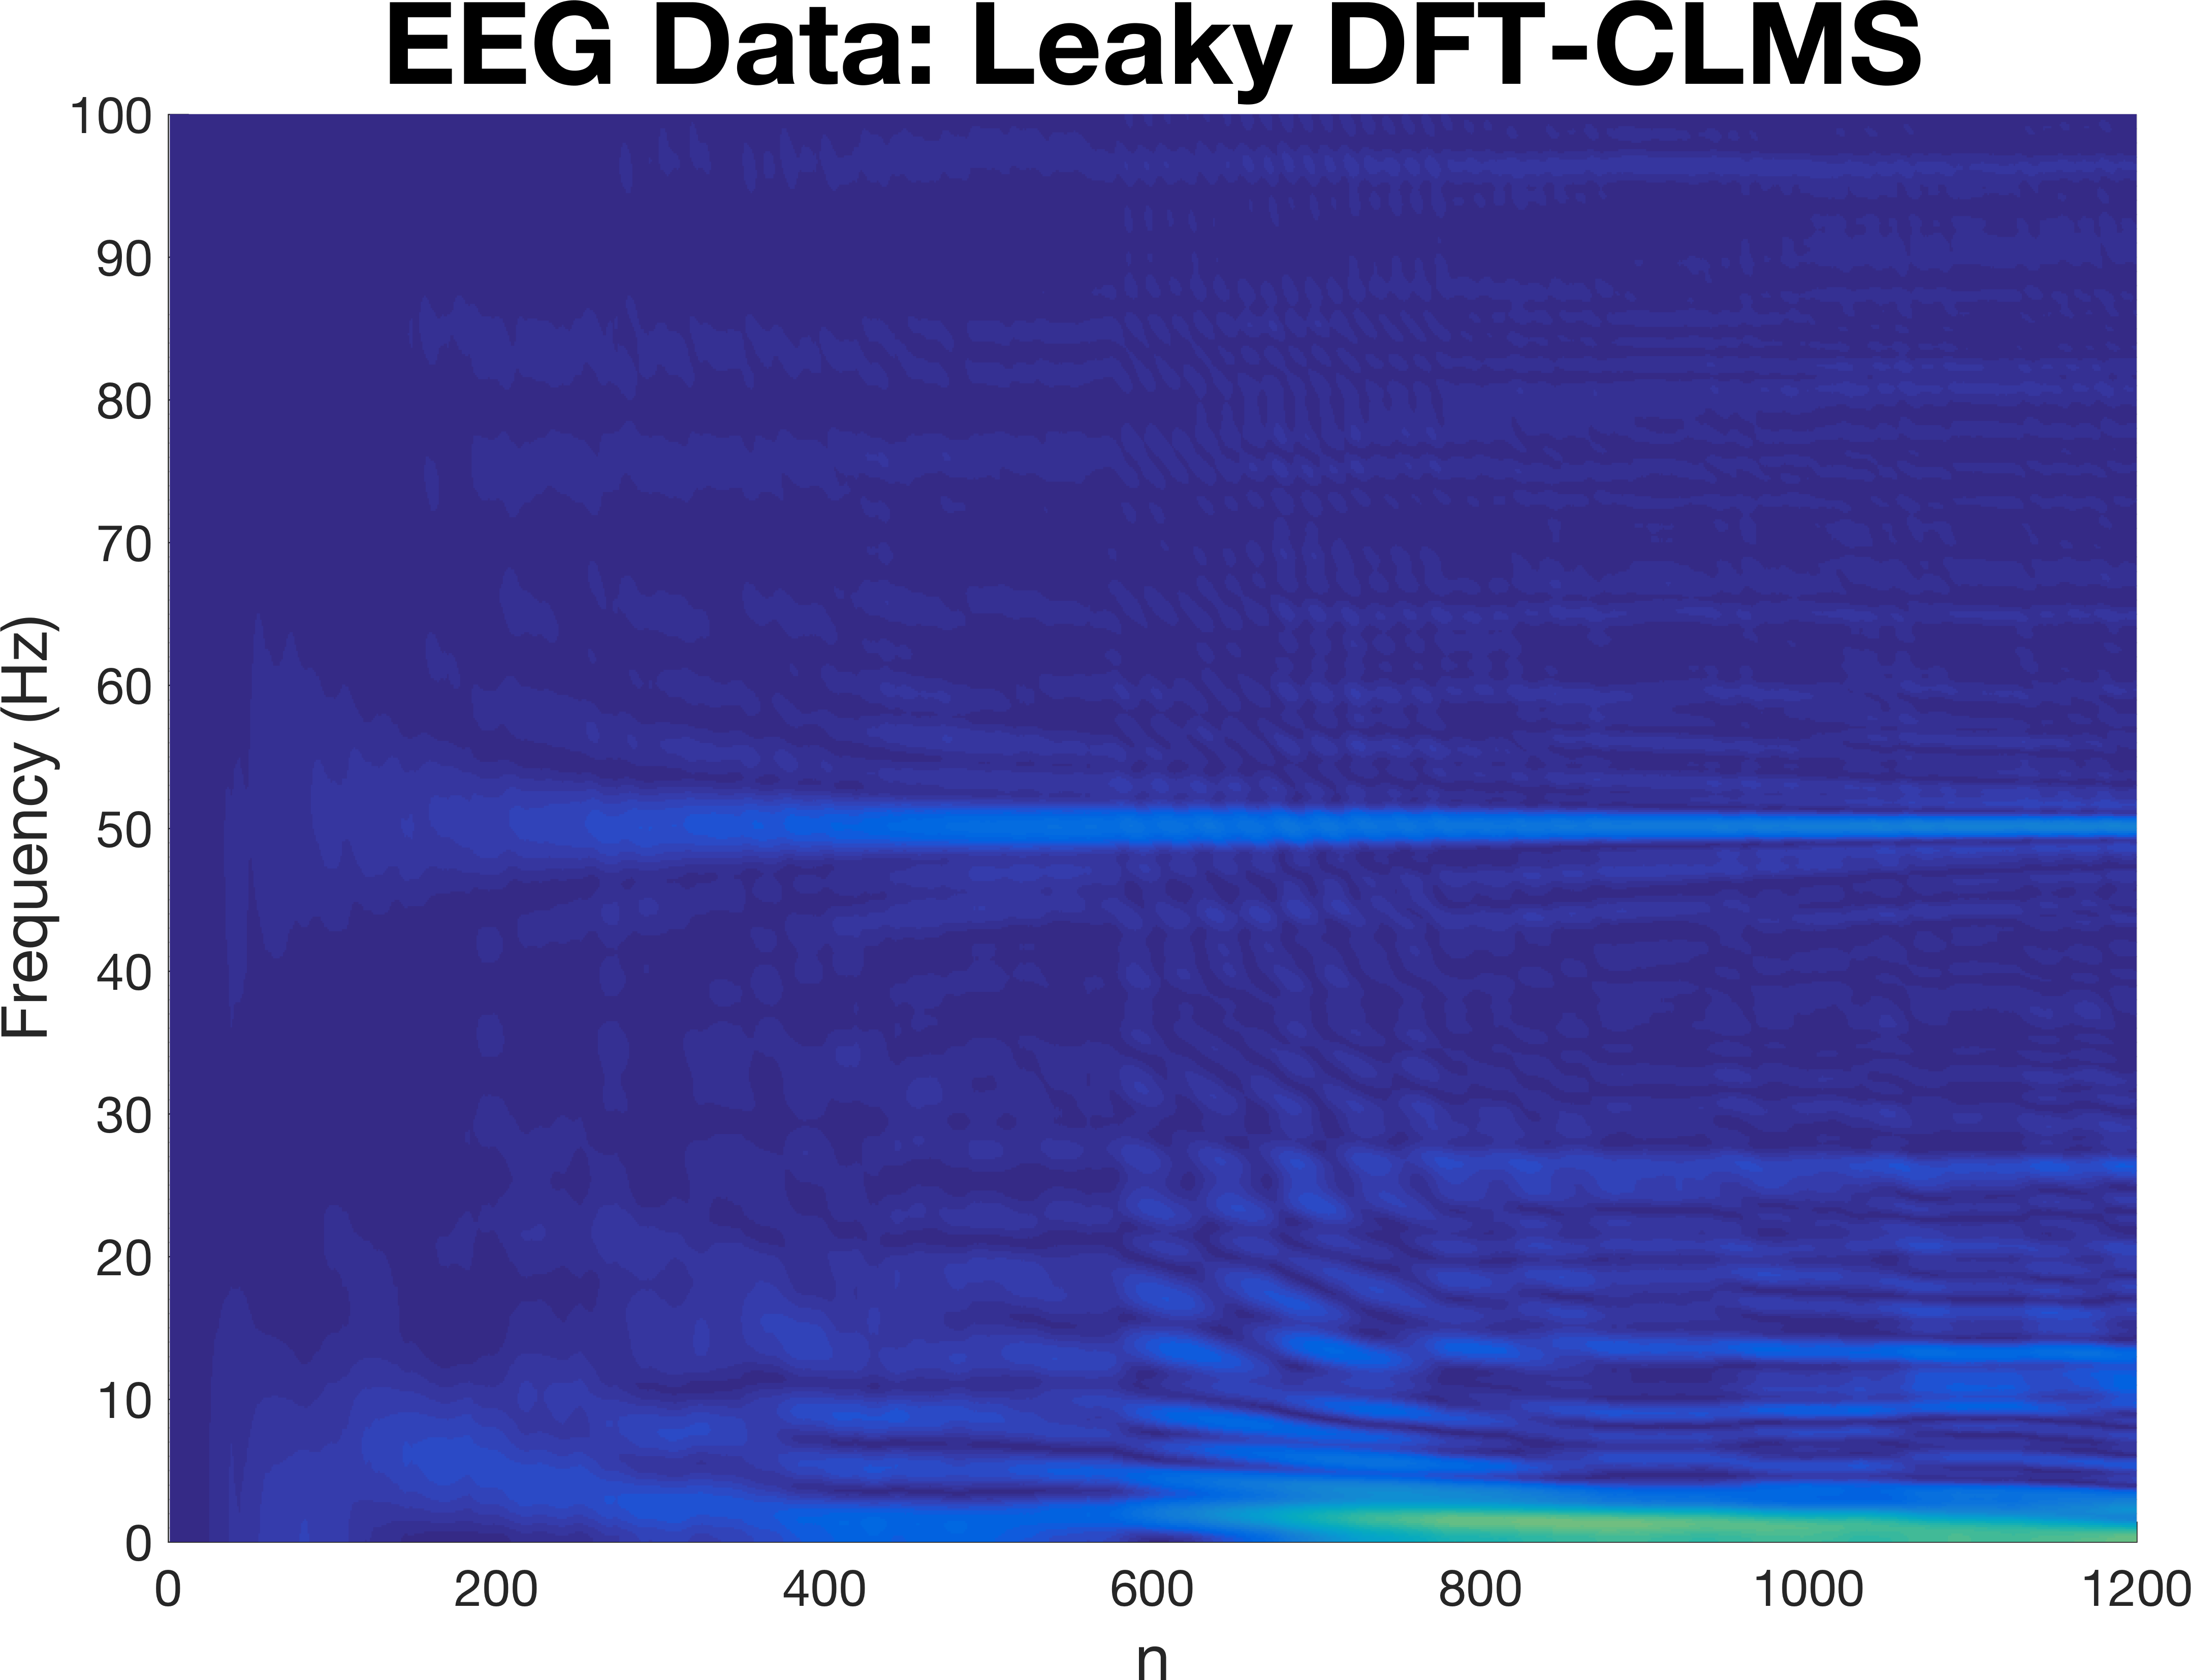
\includegraphics[width=0.32\textwidth]{part4/eeg_time_frequency_dft_leaky}
\caption{}
\end{figure}





